%%REF: https://www.sharelatex.com/blog/2013/08/02/thesis-series-pt1.html
%%REF: https://tex.stackexchange.com/questions/291156/phd-master-bachelor-thesis-which-document-class-to-choose
%\documentclass[12pt, twoside]{report}

%\documentclass[11pt]{report}
\documentclass[twoside,openright,11pt]{report}
%\documentclass[bibtotoc,liststotoc,BCOR5mm,DIV12]{scrbook}

%\usepackage{geometry}
\usepackage[english]{babel}
%\usepackage[usenames, dvipsnames]{xcolor} % for coloring fonts
\usepackage{fancyhdr}           % for header footer not used yet
%\usepackage{url}                % for printing formatted url using \url
%\usepackage{longtable}          % for multipage tables
%\usepackage{pifont}             % for printing special characters using \ding
%\usepackage{graphicx}           % for images
%\usepackage{multirow}           % for combining multiple rows in a table
%\usepackage{array}              % for table adjustments
%\usepackage[utf8]{inputenc}
%\usepackage{tikz}
%\usepackage{pgfplots}
%\usepackage{ifthen}
\usepackage{titlesec}
%\usepackage{float}
%\usepackage{tablefootnote}
%\usepackage{textcomp}
%\usepackage{palatino}
%\usepackage[acronym]{glossaries}
%\usepackage{acro}
\usepackage{emptypage}
%%%%%%%%PATCH FOR DISAPPEARANCE OF SECTION NUMBERS%%%%%%%%%%%%%%%%
\usepackage{etoolbox}
\makeatletter
\patchcmd{\ttlh@hang}{\parindent\z@}{\parindent\z@\leavevmode}{}{}
\patchcmd{\ttlh@hang}{\noindent}{}{}{}
\makeatother
%%%%%%%%%%%%%%%%%%%%%%%%%%%%%%%%%%%%%%%%%%%%%%%%%%%%%%%%%%%%%%%%%%
%%%%%%%%%%%%%%% BIBLIO IN TABLE OF CONTENTS %%%%%%%%%%%%%%%%%%%%%%
%%%%%%%%%%%%%%%%%%%%%%%%%%%%%%%%%%%%%%%%%%%%%%%%%%%%%%%%%%%%%%%%%%

\titleformat{\chapter}{\normalfont\huge\bf}{\thechapter.}{20pt}{}

\usepackage[backend=bibtex,bibencoding=ascii,style=ieee,backref=true]{biblatex}
\addbibresource{ref/references.bib}

\usepackage[usenames,dvipsnames]{xcolor} % for coloring fonts
\usepackage{url}                % for printing formatted url using \url
\usepackage{longtable}          % for multipage tables
\usepackage{graphicx}           % for images
\usepackage[utf8]{inputenc}
\usepackage{tikz}
\usepackage{pgfplots}
%\usepackage{pgfplotstable}
\usepackage{ifthen}
\usepackage{hyperref}
\usepackage{float}
\usepackage{tablefootnote}
%\usepackage{acro}
\usepackage[section,nopostdot,nonumberlist,acronym,nogroupskip]{glossaries}
%\usepackage[acronym,nohypertypes={acronym,notation}]{glossaries}

\usetikzlibrary{calc}
\usetikzlibrary{patterns}
\usetikzlibrary{positioning}
\usetikzlibrary{decorations.pathreplacing}
\graphicspath{ {img/} }

\pgfplotsset{compat=1.12,height=0.3\textheight,legend cell align=left,tick scale binop=\times}
%\pgfplotsset{grid style={loosely dotted,color=darkgray!30!gray,line width=0.6pt},tick style={black,thin}}
%\pgfplotsset{every axis plot/.append style={line width=0.8pt}}


%\DeclareAcronym{apic}{
%  short = APIC ,
%  long  = Advanced Programmable Interrupt Controller ,
%  class = abbrev
%}

%\glsaddall
%\makeglossaries % use TeX to sort
\makenoidxglossaries % use TeX to sort
\glsdisablehyper

%\setacronymstyle{long-short}
%\newglossaryentry{apic}{name={APIC},description={Advanced Programmable Interrupt Controller}}
\newacronym{apic} {APIC} {Advanced Programmable Interrupt Controller}
\newacronym{lapic} {LAPIC} {Local APIC}
\newacronym{ioapic} {IOAPIC} {I/O Advanced Programmable Interrupt Controller}
\newacronym{hpet} {HPET} {High Precision Event Timer}
\newacronym{kvm} {KVM} {Kernel-based Virtual Machine}
\newacronym{phidias} {PHIDIAS} {Provable Hypervisor with Integrated Development Information}
\newacronym{wcet} {WCET} {Worst Case Execution Time}
\newacronym{os} {OS} {Operating System}
\newacronym{gpos} {GPOS} {General Purpose Operating System}
\newacronym{rtos} {RTOS} {Real-time Operation System}
\newacronym{vm} {VM} {Virtual Machine}
\newacronym{rt} {RT} {Real-time}
\newacronym{vmm} {VMM} {Virtual Machine Monitor}
\newacronym{io} {IO} {Input/Output}
\newacronym{gpio} {GPIO} {General Purpose Input/Output}
\newacronym{isa} {ISA} {Instruction Set Architecture}
\newacronym{vmx} {VMX} {Virtual Machine Extensions}
\newacronym{vt} {VT-x} {Intel Virtualization Technology}
\newacronym{vmcs} {VMCS} {Virtual Machine Control Structure}
\newacronym{pi} {PI} {Posted Interrupt}
\newacronym{pinv} {PINV} {Posted Interrupt Notification Vector}
\newacronym{pid} {PID} {Posted Interrupt Descriptor}
\newacronym{dii} {DII} {Direct Interrupt Injection}
\newacronym{mmu} {MMU} {Memory Management Unit}
\newacronym{pml4} {PML4} {Page Map Level 4}
\newacronym{pml4e} {PML4E} {Page Map Level 4 Entry}
\newacronym{pdpt} {PDPT} {Page Directory Pointer Table}
\newacronym{pdpte} {PDPTE} {Page Directory Pointer Table Entry}
\newacronym{pd} {PD} {Page Directory}
\newacronym{pde} {PDE} {Page Directory Entry}
\newacronym{pt} {PT} {Page Table}
\newacronym{pte} {PTE} {Page Table Entry}
\newacronym{pa} {PA} {Physical Address}
\newacronym{gpa} {gPA} {Guest Physical Address}
\newacronym{ept} {EPT} {Exteneded Page Tables}
\newacronym{eptp} {EPTP} {Exteneded Page Tables Pointer}
\newacronym{cat} {CAT} {Cache Allocation Technology}
\newacronym{clos} {CLOS} {Class of Service}
\newacronym{llc} {LLC} {Last Level Cache}
\newacronym{ln} {Ln} {nth Level}
\newacronym{itlb} {iTLB} {Instruction Translation Lookaside Buffer}
\newacronym{dtlb} {dTLB} {Data Translation Lookaside Buffer}
\newacronym{xml} {XML} {Extensible Markup Language}
\newacronym{tcb} {TCB} {Trusted Computing Base}
\newacronym{ipi} {IPI} {Inter-Processor Interrupts}
\newacronym{msi} {MSI} {Message Signaled Interrupts}
\newacronym{tsc} {TSC} {Time-Stamp Counter}
\newacronym{uart} {UART} {Universal Asynchronous Receiver Transmitter}
\newacronym{irt} {IRT} {Interrupt Response Time}
\newacronym{pcie} {PCIe} {Peripheral Component Interconnect Express}
\newacronym{fpga} {FPGA} {Field Programmable Gate Arrays}
\newacronym{pc} {PC} {Personal Computer}
\newacronym{ram} {RAM} {Random Access Memory}
\newacronym{tlb} {TLB} {Translation Lookaside Buffer}
\newacronym{cpi} {CPI} {Cycles Per Instruction}
\newacronym{cdf} {CDF} {Cumulative Distribution Function}
\newacronym{msr} {MSR} {Model Specific Register}
\newacronym{sdm} {SDM} {Software Developer's Manual}
\newacronym{posix} {POSIX} {Portable Operating System Interface}
\newacronym{api} {API} {Application Programming Interface}
\newacronym{pit} {PIT} {Programmable Interval Timer}
\newacronym{irq} {IRQ} {Interrupt Request}
\newacronym{vpid} {VPID} {Virtual Process Identifiers}
\newacronym{svm} {SVM} {Secure Virtual Machine}
\newacronym{cc} {CC} {Clock Cycles}
\newacronym{wc} {WC} {Worst-case}
%\newacronym{} {} {}



\newcommand\mcachepressure{\texttt{cache\_pressure}}
\newcommand\mforkops{\texttt{forkops}}
\newcommand\mfileops{\texttt{fileops}}
\newcommand\mhackbench{\texttt{hackbench}}
\newcommand\mmmapops{\texttt{mmapops}}
\newcommand\mstdout{\texttt{stdout}}
\newcommand\mthreadops{\texttt{threadops}}
\newcommand\mnoload{\texttt{no load}}

\newcommand\mextint{\texttt{ext\_int}}
\newcommand\mwrmsr{\texttt{wrmsr}}
\newcommand\mcpuid{\texttt{cpuid}}
\newcommand\mcrxaccess{\texttt{crx\_access}}
\newcommand\mextinterrupt{\texttt{ext\_interrupt}}

\newcommand\mVMXON{\texttt{VMXON}}
\newcommand\mINVVPID{\texttt{INVVPID}}
\newcommand\mVMLAUNCH{\texttt{VMLAUNCH}}
\newcommand\mVMREAD{\texttt{VMREAD}}
\newcommand\mVMWRITE{\texttt{VMWRITE}}


\newif\ifreport
\newif\ifdefense

\reporttrue

%%commands latency reduction plots%%%%
\newcommand\figheight {8cm}
\newcommand\figwidth  {13.5cm}
\newcommand\ybarXdist {2.3cm}
\newcommand\ybarWidth {16pt}
\newcommand\ybarSep {2pt}
\newcommand\xShiftLatency {0cm}
\newcommand\xShiftImprove {0.7cm}
\newcommand\atCmdLowerPlot {at={($(plot1.west)+(0,-10.5cm)$)}}
%%commands for virtualization overhead plots %%%%
\newcommand\ybarWidthVO {15pt}
\newcommand\atCmdVOverheadLowerPlot {at={($(plot1.west)+(0,-11.5cm)$)}}
\newcommand\ybarSepVO {3pt}
\newcommand\ybarXdistVO {1.3cm}
%%commands for virtualization overhead CDF plots %%%%
\newcommand\atCmdVOCDFLowerPlotA {at={($(plot1.south west)+(0,-6.5cm)$)}}
\newcommand\atCmdVOCDFLowerPlotB {at={($(plot2.south west)+(0,-6.5cm)$)}}
\newcommand\figheightVOCDF {6cm}
\newcommand\figwidthVOCDF {12cm}
%%commands for virtualization overhead CDF plots in appendix %%%%
\newcommand\figheightVOCDFApp {7cm}
\newcommand\figwidthVOCDFApp {12cm}
\newcommand\atCmdVOCDFLowerPlotAApp {at={($(plot1.south west)+(0,-7.5cm)$)}}
\newcommand\atCmdVOCDFLowerPlotBApp {at={($(plot2.south west)+(0,-7.5cm)$)}}

%%https://tex.stackexchange.com/questions/67446/change-colour-of-boxes-surrounding-links-in-hyperref
%%\usepackage{hyperref}

%% Page Dim (A4): 210 × 297
%%bindingoffset=0.4in
\usepackage[a4paper,left=30mm,width=150mm,top=30mm,bottom=30mm]{geometry}
%\usepackage[english]{babel}
\hypersetup{
    %hyperfootnotes=false
    linkbordercolor=blue!30,
    allbordercolors=blue!30,
    %backref=true,
    backref=page,       
    pagebackref=true,               
    hyperindex=true, 
    %colorlinks=true,                
    breaklinks=true,                
    urlcolor= black,                
    linkcolor= black,                
    bookmarks=true,
    bookmarksopen=false,
    filecolor=black,
    citecolor=black,
}


%\pagestyle{fancy}
%\fancyhf[RE,RO,LO,LE,C]{}
%\fancyfoot[R]{\thepage} %% clear out all footers
%\fancyhead[RE]{\nouppercase{\leftmark}}
%\fancyhead[LO]{\nouppercase{\rightmark}}

%\fancyhf{}
%\rhead{}
%\lhead{}
%\rfoot{\thepage}

%\makeglossaries

\begin{document}

%%%%%%%%%%%%%%%%%%%%%%PREAMBLE%%%%%%%%%%%%%%%%%%%%%%%
\begin{titlepage}
    \begin{center}
        \vspace*{0.5cm}

        
\includegraphics[width=0.4\textwidth]{tu_logo} \\
		\vspace{0.25cm}
		\textnormal{Fakult{\"a}t f{\"u}r Elektrotechnik und Informatik} \\
		\textnormal{Institut f{\"u}r Softwaretechnik und Theoretische Informatik} \\
		\textnormal{Fachgebiet Security in Telecommunications} \\
		\vspace{1.0cm}
		\textbf{\Large{Masterarbeit}}\\
		\vspace{1.0cm}
		\textbf{\LARGE{Latency Reduction using Intel CAT in Virtualized Environment}} \\
		\vspace{1.5cm}
		\textnormal{\large{presented by}} \\
        \textnormal{\Large{Muhammad Waseem Arshad}} \\
        \textnormal{\large{student ID: 387428}} \\
		\textnormal{\large{student of}}\\ 
		\textnormal{\Large{Masterstudiengang ICT Innovation}} \\
		\textnormal{\large{Embedded Systems}} \\
		%\textnormal{\large{\today}} \\
		%\textnormal{\large{from Faculty IV - Electrical Engineering and Computer Science}} \\
		%\textnormal{\large{at Technische Universit{\"a}t Berlin}} \\
		\vspace{1.0cm}
		\textnormal{\large{for obtaining the academic degree}} \\
		\textnormal{\Large{Master of Engineering}} \\
		\vspace{2cm}
		\textnormal{\large{Betreuender Hochschullehrer: Prof. Dr. Jean-Pierre Seifert}} \\
		\textnormal{\large{Sek. Betreuender Hochschullehrer: Prof. Dr. Ben Juurlink}} \\
		\textnormal{\large{Betreuender Mitarbeiter: M.Sc. Robert Buhren}} \\
		\vspace{2cm}
		%\textnormal{\large{Technische Universit{\"a}t Berlin}} \\
		%\textnormal{\large{Fakult{\"a}t IV}} \\
		%\textnormal{\large{Institut f{\"u}r Softwaretechnik und Theoretische Informatik}} \\
		%\textnormal{\large{Professur Security in Telecommunications}} \\
		\textnormal{\Large{Berlin}}\\
		\textnormal{\Large{\today}}\\
        
    \end{center}
\end{titlepage}

\clearpage{\thispagestyle{empty}\cleardoublepage}

\pagenumbering{roman}

%\vspace*{4cm}
\chapter*{Erkl{\"a}rung}
%I hereby declare that I am carrying out the presented work independently and by myself without 
%unauthorized third-party assistance and solely using the listed sources and tools.
Hiermit erkl{\"a}re ich, dass ich die vorliegende Arbeit selbstst{\"a}ndig und eigenh{\"a}ndig sowie ohne unerlaubte fremde Hilfe und ausschlie{\ss}lich unter Verwendung der aufgef{\"u}hrten Quellen und Hilfsmittel angefertigt habe.
\newline
\newline
\newline
Berlin, %\today %19 March 2016
\newline
\newline
\newline
\newline
\newline
Muhammad Waseem Arshad


\clearpage{\thispagestyle{empty}\cleardoublepage}


\chapter*{Abstract}
Embedded systems are deeply integrated into our society to an extent that we tend to forget about their existence.
These systems have improved quality of life and increased human productivity through automation.
Many applications that run on these devices have real-time requirements subjected to stringent timing constraints.
Real-time application used to be simple and usually ran on single core processors, but this is not true anymore. 

Recent technological trends like \emph{"Industry 4.0"} and \emph{"Internet of Things"}
has steered real-time system designers to support networking.
These improvements have led to the increased complexity of software stack and demand secure 
mechanisms to achieve system reliability.
Advancements in multicore processor technology have found its way to embedded systems. 
System designers have embraced multicore technology and more real-time application run on multicore architectures than ever before.
Multicore technology has brought a new set of opportunities.
Applications of mixed-criticality that used to run on separate hardware platforms can be consolidated on one platform.
Real-time applications can be assigned to dedicated processor core(s) to ensure spatial isolation. 
The solution is equally valid for the legacy applications, given their execution behavior
is not affected.

A classical solution to consolidate application on one platform is Virtualization.
For many years virtualization has been used in server and cloud computing to host multiple applications
on the single machine.
Recently virtualization has acquired acceptance in the embedded domain for application consolidation.
Consolidation allows system designers to reduce system costs, and utilize huge amounts of processing power available in one chip.
However, virtualization solutions that are widely accepted in enterprise domain are not applicable to the
real-time system. 
These solutions are designed to increase the average throughput of the software system.

Real-time systems are evaluated based on worst-case response times to handle an event.
Since real-time systems are subjected to stringent timing constraints, a virtualization
solution for the real-time system has to guarantee deterministic response times.
A faithful virtualization solution suitable for the real-time system has to
be aware of real-time constraints. A hypervisor should keep small footprint and 
has to ensure temporal and spatial isolation of virtualized applications.

Phidias is a statically configurable hypervisor that follows microkernel and multikernel design models.
The hypervisor keeps low complexity and memory footprint by deploying the principle of staticity.
While the hypervisor follows design principles that are favorable to real-time applications, its real-time capabilities are unknown.
This thesis confirms real-time capabilities of Phidias hypervisor on the x86 platform
by measuring virtualization overhead for a real-time guest. 
Furthermore, the thesis presents performance tuning
mechanisms to reduce interrupt response times of real-time guest. 
The results show that latency reduction techniques used can significantly reduce the virtualization overhead.

\clearpage{\thispagestyle{empty}\cleardoublepage}

\chapter*{Zusammenfassung}

Eingebettete Systeme sind tief in unsere Gesellschaft integriert, daher neigen wir dazu ihre Existenz nicht mehr wahr zu nehmen.
Diese Systeme verbesserten die Lebensqualit{\"a}t und eine erh{\"o}hten die menschliche Produktivit{\"a}t durch Automatisierung.
Viele Anwendungen, die auf diesen Ger{\"a}ten ausgef{\"u}hrt werden, haben Echtzeitanforderungen, die strengen Timing-Einschr{\"a}nkungen unterliegen.
Echtzeitanwendungen waren fr{\"u}her einfach und liefen normalerweise auf Single-Core-Prozessoren, dies ist heutzutage nicht mehr der Fall.

Aktuelle Trends wie \emph{"Industrie 4.0"} und \emph{"Internet of Things"} f{\"u}hren zu einer vermehrten Vernetzung von Echtzeit-F{\"a}higen Systemen.
Diese Entwicklung hat zu einer erh{\"o}hten Komplexit{\"a}t des Software-Stacks gef{\"u}hrt und verlangt die Entwicklung neuer
Mechanismen, um die Systemzuverl{\"a}ssigkeit zu erreichen.
Desweiteren haben Fortschritte in der Multicore-Prozessortechnologie ihren Weg in eingebetteten Systemen gefunden.
Systemdesigner haben sich f{\"u}r Multicore-Technologie entschieden und es laufen so viele Echtzeitanwendungen auf Multicore-Architekturen wie nie zuvor.
Die Multicore-Technolo-gie hat neue M{\"o}glichkeiten er{\"o}ffnet.
Anwendungen gemischter Kritikalit{\"a}t, die fr{\"u}her auf separaten Hardwareplattformen ausgef{\"u}hrt wurden, k{\"o}nnen auf einer Plattform konsolidiert werden.
Echtzeitanwendungen k{\"o}nnen dedizierten Prozessorkernen zugewiesen werden, um eine r{\"a}umliche Isolierung zu gew{\"a}hrleisten.
Diese L{\"o}sung ist f{\"u}r Legacy-Anwendungen gleicherma{\ss}en g{\"u}ltig, sofern sich ihr Ausf{\"u}hrungsverhalten nicht {\"a}ndert.

Eine klassische L{\"o}sung zur Konsolidierung mehrerer Anwendungen auf einer Plattform ist Virtualisierung.
Seit vielen Jahren wird Virtualisierung in den Bereichen Server- und Cloud-Computing eingesetzt, um mehrere Anwendungen auf einer einzigen Maschine zu hosten.
In letzter Zeit hat sich Virtualisierung auch bei eingebettete Systeme  f{\"u}r die Anwendungskonsolidierung etabliert.
Durch die Konsolidierung k{\"o}nnen Systementwickler die Systemkosten reduzieren und die volle Rechenleistung auf einem Chip nutzen.
Allerdings sind Virtualisierungsl{\"o}sungen, die in der Unternehmensdom{\"a}ne weit verbreitet sind, nicht direkt auf Echtzeit-Systeme {\"u}bertragbar.
Diese L{\"o}sungen sollen den durchschnittlichen Durchsatz des Softwaresystems erh{\"o}hen.

Im Gegensatz dazu werden Echtzeitsysteme hinsichtlich der Antwortzeiten im worst-case Fall optimiert.
Da Echtzeitsysteme strengen zeitlichen Einschr{\"a}nkungen unterliegen muss eine L{\"o}sung f{\"u}r Echtzeitsystem eine deterministische Antwortzeit garantieren.
Eine f{\"u}r das Echtzeitsystem geeignete, zuverl{\"a}ssige Virtualisierungsl{\"o}sung muss diese Echtzeitanforderung erf{\"u}llen.
Ein Hypervisor sollte einen geringen Platzbedarf ben{\"o}tigen und muss die zeitliche und R{\"a}umliche Isolierung von virtualisierten Anwendungen gew{\"a}hrleisten.

Phidias ist ein statisch konfigurierbarer Hypervisor, der Microkernel-und Multikernel-Designmodellen folgt. 
Der Hypervisor minimiert die Komplexit{\"a}t und den Speicherbedarfdurch ein vollst{\"a}ndig statisches Design. 
W{\"a}hrend der Hypervisor Designprinzipien folgt, die f{\"u}r Echtzeitanwendungen g{\"u}nstig sind, sind seine tats{\"a}chlichen
Echtzeitf{\"a}higkeiten unbekannt. Diese Arbeit best{\"a}tigt die Echtzeitf{\"a}higkeiten von Phidias Hypervisor auf der x86-Plattform
durch Messen des Virtualisierungsoverheads f{\"u}r einen Echtzeitgast. Des Weiteren pr{\"a}sentiert die Arbeit Leistungsoptimierung
Mechanismen zur Reduzierung der Interrupt-Antwortzeiten von Echtzeit-Gast.
Die Ergebnisse zeigen, dass Latenzreduktionstechniken den Virtualisierungsaufwand deutlich reduzieren k{\"o}nnen.

\clearpage{\thispagestyle{empty}\cleardoublepage}

%\chapter*{Dedication}
To mum and dad

%\clearpage{\thispagestyle{empty}\cleardoublepage}

\chapter*{Acknowledgments}
I want to thank everybody at SecT group for providing a wonderful opportunity.
Thanks to Robert Buhren for mentoring and helping us finish thesis in time.
Special thanks to Jan Nordholz for his assistance in understanding Phidias hypervisor.
I would also like to thank Julian Fietkau for his assistance in setting up latency measurement setup and instrumentation tools he provided.
The Linux logo (Tux) was created by Larry Ewing, Simon Budig, Anja Gerwinski, and ’The GIMP’.
UART module used for communication between FPGA and external PC is designed by Dmitri Nedospasov and Thorsten Schroeder.

\clearpage{\thispagestyle{empty}\cleardoublepage}

%%%%%%%%%%%%%%%%%%%%%%%%%%%%%%%%%%%%%%%%%%%%%%%%%%%%%
\pagestyle{fancy}
\fancyhf[RE,RO,LO,LE,C]{}
\fancyfoot[R]{\thepage} %% clear out all footers
\fancyhead[RE]{\nouppercase{\leftmark}}
\fancyhead[LO]{\nouppercase{\rightmark}}
%%%%%%%%%%%%%%%%%%%%%%%%%%%%%%%%%%%%%%%%%%%%%%%%%%%%%
\tableofcontents
\clearpage{\thispagestyle{empty}\cleardoublepage}

\listoffigures 
\clearpage{\thispagestyle{empty}\cleardoublepage}

\listoftables
\clearpage{\thispagestyle{empty}\cleardoublepage}


%%%%%%%%%%%%%%%%%%%%%%%%%%%%%%%%%%%%%%%%%%%%%%%%%%%%%
\pagestyle{fancy}
\fancyhf[RE,RO,LO,LE,C]{}
\fancyfoot[R]{\thepage} %% clear out all footers
\fancyhead[RE]{\nouppercase{\leftmark}}
\fancyhead[LO]{\nouppercase{\rightmark}}
%%%%%%%%%%%%%%%%%%%%%%%%%%%%%%%%%%%%%%%%%%%%%%%%%%%%%
%%%%%%%%%%%%%%%%%%%%%%CHAPTERS%%%%%%%%%%%%%%%%%%%%%%%
\pagenumbering{arabic}


\newcommand\moreslaw{Law states that number of transistors on a chip doubles approximately every two years}
\newcommand\IoT{A trend that aims to connect everything to the cloud}
\newcommand\industry{A trend that aims to enable machine to machine communication and connecting machines to cloud}

\chapter{Introduction \label{chap1}}

Embedded systems has drastically improved productivity, safety, and comfort of an average human being.
When we are inside the building they regulate temperature and humidity to our desires, 
they keep the intruders away and alarm us in critical situations. 
When we are outside, they monitor and control engine and brake system of the car, bus, train or airplane.
At work, they automate and regulate the processes without too much human intervention.
They entertain us when we are well and help diagnose the illness if we are sick.
In fact every aspect of human is affected by embedded systems.
%Embedded systems are integrated to our everyday life and they are designed so well that we tend to forget about their existense.

Most of these embedded systems are real-time which means, for simplicity at this point, having stringent time constraints.
Deterministic response times is the key design aspect
that makes them different from traditional computing devices like desktop and server computers.
Furthermore, real-time applications are designed and evaluated based on the worst case event handling latency and execution times, while
in desktop and server computers applications are optimized for average case execution time.
Real-time operating systems or a custom tailored software solutions are used for real-time applications to guarantee these requirements.
Often multiple embedded devices has been used to isolate constraints imposed on one real-time application from another.
An example is car infotainment system. Traditionally dedicated computing systems has been used to isolate 
control and monitoring the car subsystems from computing system responsible for entertainment solutions.
The traditional landscape is changing due to emerging technological changes in the computing systems.


For many years designers improved processor performance by putting more transistor on a single chip, exploiting More's Law\footnote{\moreslaw}, and increasing the clock frequency.
Almost a decade ago chip designers had to stop increasing clock frequencies due to power limitations.
As they could still put more transistors on a single chip, designers started adding multiple cores on a single chip.
Hence a new era of multicore computing begun and by now multicore processors has become a norm.
The multicore trend has led to a new set of challenges and opportunities for real-time embedded systems.
Availability of multiple processing elements in a single chip enables consolidation of real-time applications with other applications.
Consolidation of real-time applications can help reduce design complexity, costs and power consumption.
However it poses a new challenge which is how to ensure temporal and spacial isolation of different applications running on the same platform.

Embedded systems used to be small and simple and software stacks for these devices were relatively simpler
than general purpose computing devices. But it is not true anymore.
In the past few years, embedded systems has embraced internet. New technological trends like \emph{Internet of Things}\footnote{\IoT} and \emph{Industry 4.0}\footnote{\industry}
has steered embedded systems to become part of a networked system.
Therefor, embedded systems are becoming increasingly complex much like traditional computer systems.
Even though network connectivity has improved the overall system performance and provided opportunities for innovative solutions to many challenges industry faced,
it also poses threat to the integrity of the system.
These systems has become accessible to the outside world, and intruders or malignant applications can compromise the whole system.

Virtualization is a technique that allows hosting multiple virtual machines on one physical machine. 
It has been around of decades and historically used to consolidate multiple server applications on a single machine.
Virtualization enables system designers to minimize the effects of security threats 
by providing ease in threat detection, localizing and isolating compromised virtual machine from the others preventing overall system failure \cite{Chen:2001:VBR:874075.876409}.
Recently virtualization has gained popularity in embedded systems domain.
Virtualization has potential to provide solutions to the emerging challenges for embedded systems \cite{Heiser:2008:RVE:1435458.1435461}.
Applications of mixed criticality (real-time and non real-time) can be consolidated on a single platform by executing each 
application in a separate virtual machine.
Virtualization can also solve potential security risks to the real-time applications.

Virtualization has great advantages, however they come at the cost of increased overhead. 
The responsiveness of the real-time application can be affected. 
The virtual machine monitor or hypervisor has to ensure isolation of real-time application from
other applications running on the same hardware and keeping the application's response time 
close to when running it native. Several virtualization solutions has been proposed for real-time application
in the past few years. Most solutions are based on existing time-shared operating system (e.g. KVM, Jailhouse), while some 
use microkernel-based approach to keep the hypervisor footprint and critical paths to minimum (e.g. OKL4).

An innovative solution that follows microkernel approach PHIDIAS hypervisor. 
The hypervisor is developed by Jan Nordholz at Security in Telecommunications chair, TU Berlin.
The hypervisor follows some key design principles that makes it very attractive for the embedded market.
It supports static partitioning of hardware resources to virtual machines.
And removes much of the dynamic components of hypervisor by generating data structures like page-tables statically, hence removing dynamic memory allocater altogether.
The principle of staticity used in Phidias design allows reducing dynamic components and eases provability of the hypervisor.
The software provability has significant importance to real-time applications that are frequently subjected to various certifications.

This thesis evaluates performance of real-time virtualization solution based on Phidias hypervisor on x86 platform.
Phidias is a successor of Perikles hypervisor also developed at Security in Telecommunications chair, TU Berlin.
A similar study was conducted for Perikles hypervisor on ARMv7 architecture.
Perikiles is already undergoing integration in an industrial product \cite{opensynergy_coqos}.
Although ARM processors dominate most of the embedded market, but many complex and compute extensive real-time applications use x86 platform. 
An example is industrial robotic-arm movement control. 
%%Compared to ARM, x86 enjoys rich 
The x86 architecture is also finding its way into automotive industry where workloads have become very complex than ever before.


The objectives of this thesis are twofold: to measure virtualization overhead and use various mechanisms to lower the overhead.
To improve real-time responsiveness of the applications this thesis evaluates following techniques:
\begin{itemize}
\item \textbf{Direct interrupt injection} will be used to deliver device interrupts owned by the guest without hypervisor intervention.
\item \textbf{Partitioning of shared last-level cache} will be used for spacial isolation of real-time guest from other guests.
\item \textbf{Partitioning of TLB} will be used for spacial isolation of real-time guest from the hypervisor itself.
\end{itemize}


The thesis is organized as follows. 
Chapter \ref{chap2} covers background of real-time systems, virtualization technology, latency reduction mechanisms, and 
design and implementation of Phidias hypervisor.
Chapter \ref{chap3} presents presents details of real-time virtualization system used to measure overhead and reports the results.
The performance improvements using latency reduction mechanisms are reported in Chapter \ref{chap4}.
Chapter \ref{chap5} gives an account of related work and Chapter \ref{chap6} concludes this thesis.

%% \section{Purpose}
%% This chapter will give a comprehensive introduction to thesis topic and material covered in the report.
%% The problem will be introduced by giving:
%% \begin{itemize}
%% \item importance of embedded systems
%% \item how design principles of virtualization techniques differ for embeddded applications from other application like servers
%% \item significance of embedded hypervisors
%% \item a very brief intro to Phidias
%% \end{itemize}
%% The solution will be introduced by giving brief introdcution to:
%% \begin{itemize}
%% \item cache allocation technology by Intel
%% \item posted interrupt mechanism
%% \item test enviorment
%% \end{itemize}


\chapter{Background\label{chap2}}

\section{Real-time Systems}
A real-time embedded system consists of computational tasks that are bounded by time constraints. The time constraint is dictated by the environment in which the real-time system is integrated. 
Kopetz \cite{Kopetz:2011:RSD:1995310} has defined real-time system as follows:

\emph{"real-time system is a computer system in which the correctness of the system behavior depends not only on the logical results of the computations, but also on the physical instant at which these results are produced"}. 


The system works correctly as long as the results are logically correct and produced within prescribed timing constraints. 
A task is a piece of workload that the real-time system has to execute within prescribed timing constraints. 
The real-time computing system can be designed to perform a single or multiple tasks. 
Behavior of a real-time system can be well understood by understanding characteristics of real-time tasks. 
Every real-time task is imposed by a time constraint called \emph{deadline}. 
The real-time system is supposed to complete real-time tasks before deadline of a task passes.
The time instance when a real-time task becomes ready for execution is called \emph{release time}. 
The difference between release time and the instant of time when the real-time task handler is scheduled to compute workload is called latency.
The maximum or worst-case time needed to complete the task after it is scheduled is called "response time" also called as worst-case execution time (WCET). 
Figure \ref{fig-rt-task-param} demonstrates response time of real-time task under normal circumstances assuming latency is zero. 

\begin{figure}[!htb]
\begin{center}
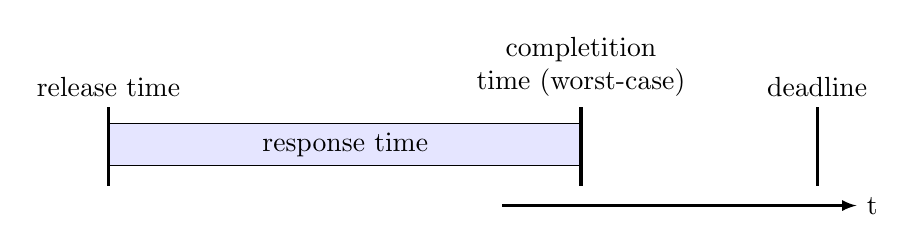
\begin{tikzpicture}

\node at (0,0.25)[rectangle, draw=black, fill=blue!10, minimum height = 0.5cm, minimum width = 6cm, anchor=south west] (resptime) {response time};
\draw[black, very thick, solid] (0,0) -- (0,1) node [above] {release time};
\draw[black, very thick, solid] (6,0) -- (6,1) node [above, text width=4cm, text centered] {completition time (worst-case)};
\draw[black, very thick, solid] (9,0) -- (9,1) node [above] {deadline};

%\node (rtlabel) at (5,-1.5) {response time};
\begin{scope}[>=latex]
	%%\draw [thick, ->] (rtlabel) to [bend left=45] (resptime.center);
	\draw[black, thick, ->] (5,-0.25) -- (9.5,-0.25) node [right] {t};
\end{scope}
\end{tikzpicture}
\end{center}
\ifreport
\caption{Response time of a real-time task}
\fi
\label{fig-rt-task-param}
\end{figure}


Deadline of a real-time task is categorized into three types: soft, firm and hard. 
The deadline is firm, if missing the deadline makes the result unusable, soft if result is still usable. 
A hard deadline means missing it would disrupt the system functionality resulting in a failure of the system.
Real-time systems are often categorized into soft and hard real-time systems based on the type of deadlines tasks are supposed to meet.
A hard real-time system consists of at least one task with hard deadline. 
A safety-critical system is hard real-time system where system failure can cause a disaster.
On contrary, all tasks in soft real-time system has soft or firm deadlines. 
Nevertheless, missing a deadline in soft as well as hard real-time systems is undesirable.

There are two types of real-time tasks based on release times: periodic and aperiodic.
A periodic real-time task is released after same interval of time and aperiodic task has irregular and unpredictable release times.
An example of periodic task is a periodic timer tick that triggers scheduling events.
And example of aperiodic task is arrival of external interrupt.
Most of the tasks in a real-time systems are performed in response to external event or stimulus and they are aperiodic.
While some are periodic and generally performed on periodic timer interrupts.
When an external event occurs the release time observed by the system is different from the actual release time due to hardware and scheduling overhead. 
The time that elapses between actual release time of the event and time instant at which the system notices the event is called \emph{interrupt latency}. 

\begin{figure}[!htb]
\begin{center}
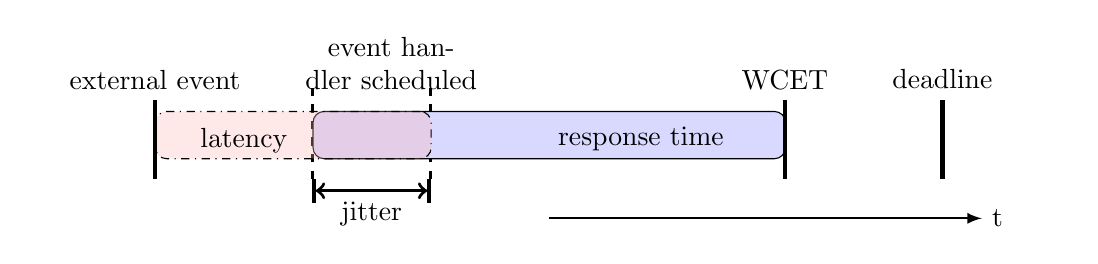
\begin{tikzpicture}
%\draw[gray, very thick, solid, >-<]  (0,1.5) -- (9,1.5) node at (4,1.5) [above] {relative deadline};
%\draw[black, very thick, ->]  (0,0) -- (10,0) node at (11,0) {time};
\draw[black, very thick, dashed] (2.0,0) -- (2.0,1.25) node at (3,1) [text width=3cm, above, align=center] {event handler scheduled};
\draw[black, very thick, dashed] (3.5,0) -- (3.5,1.25);

\node at (2.0,0.25)[rectangle, draw=black, fill=blue!15, rounded corners, minimum height = 0.6cm, minimum width = 6cm, anchor=south west] (resptime) {};

\begin{scope}[fill opacity=0.3]
\node at (0,0.25)[rectangle, draw=black, dashdotted, fill=red!30, rounded corners, minimum height = 0.6cm, minimum width = 3.50cm, anchor=south west] (latency) {};
%\node at (2.0,0.25)[rectangle, draw=black, postaction={pattern=north east lines}, minimum height = 0.6cm, minimum width = 1.5cm, anchor=south west] (overlap) {};
\end{scope}

\node [above left, inner sep=2pt] at (latency.south) {latency};
\node [above right, inner sep=3pt] at (resptime.south) {response time};

\draw[black, very thick, solid] (0,0) -- (0,1) node at (0,1) [text width=3cm, above, align=center] {external event};
\draw[black, very thick, solid] (8,0) -- (8,1) node at (8,1) [text width=3cm, above, align=center] {WCET};
\draw[black, ultra thick, solid] (10,0) -- (10,1) node at (10,1) [text width=3cm, above, align=center] {deadline};

\draw[black, very thick, solid, |<->|] (2.0,-0.15) -- (3.5,-0.15) node (jitter) at (2.75,-0.15) [below] {jitter};

%\node (latlabel) at (1,-1.0) {latency};
%\node (jitlabel) at (4,-1.0) {jitter};
%\node (rtlabel) at (8,-1.0) {response time};

\begin{scope}[>=latex]
	%\draw [thick, ->] (latlabel) to [bend right=45] (latency.center);
	%\draw [thick, ->] (rtlabel) to [bend left=45] (resptime.center);
    	%\draw [thick, ->] (jitlabel) to [bend left=45] (jitter.center);
	\draw[black, thick, ->] (5,-0.5) -- (10.5,-0.5) node [right] {t};
\end{scope}
\end{tikzpicture}
\end{center}
\ifreport
\caption{Real-time task interrupt latency and jitter}
\fi
\label{fig-latency-jitter}
\end{figure}


The interrupt or event handling latency is not a fixed parameter. The variance of interrupt latency depends on current state of the system, e.g. if system is executing a high priority task then observed release time of the event is delayed until execution of a high priority task finishes. 
The interrupt latency also depends on hardware overhead, which can vary when multiple interrupts arrive at the same time and hardware posts them one by one based on their priority.
Designers of a real-time system software are supposed to keep the event handling latency within certain bounds to respect timing constraints. 
The variance of interrupt latency is usually referred as jitter. Figure \ref{fig-latency-jitter} shows relationship of interrupt latency and latency jitter with rest of parameters.

In contrast to desktop and server application, real-time applications are designed to have deterministic response times.
The general purpose computing tasks are optimized for average running time. 
While a real-time task is optimized to have deterministic response time even at the expense of increased average-case running time.
Performance of real-time application is always evaluated based on worst-case execution times.
The difference leads to a separate class of operating systems called real-time operating systems (RTOS) specifically designed to have deterministic properties.
Characteristics of RTOS are described in the next section.


\section{Real-Time Operating Systems} \label{sec:rtos-and-types}
The operating system, or general purpose operating system (GPOS), is a piece of software that manages resources of hardware platform and provides a nice abstraction to application software for using these resources \cite{Tanenbaum:2014:MOS:2655363}. Kernel-based design is a common design approach for GPOS. The OS implements two completely isolated work spaces: kernel-space and user-space. The OS layer that manages the hardware and provides services to userspace makes up the kernel-space. The user application reside in userspace and use services provided by the OS kernel. In kernel-based OS design, typical services provided to userspace applications by OS kernel are process management, inter-process communication, time management, interrupt handling, process synchronization. 

Real-time application typically execute on top of a real-time operating system (RTOS). 
The RTOS has the same responsibilities as general purpose operating system, however the resource management and scheduling policies are usually different to guarantee deterministic behavior and respect timing constraints of real-time tasks.
%%The real-time operating systems are designed to be predictable such that the timing constraints of real-time applications are respected.
Various design approaches has been used to design RTOS.
Following sections briefly shed light on most common design approaches.

\subsection{Pure Real-time Operating Systems}
A large number of operating systems are designed exclusively for real-time applications.
Pure RTOS are typically designed to target single or a few similar real-time applications. 
For example Contiki RTOS \cite{Dunkels:2004:CLF:1032658.1034117} is designed specifically for wireless sensor nodes and it is optimized for small footprint and power efficiency.
Purposely built real-time operating systems come in many varieties: some are designed for small foot-print suited for embedded devices, and some for safety-critical applications like control of a nuclear power plant.
Many RTOSs are designed for small devices that use micro-controllers whiteout MMU support and occupy memory in the order of few tens of kilo-bytes. Examples from this class are Nucleus RTOS, $\mu$C/OS-III and Contiki.
On the other hand RTOSs like VxWorks support high-end processor families with MMU (x86, ARM, MIPS, and PowerPC). 
Often these RTOSs are rich in library content to support complex devices like graphical displays.
Most of real-time operating systems from this category are commercial and proprietary. However there are some RTOS that are open-source.
FreeRTOS is an an open-source RTOS that belong to this category.

\subsection{Extensions to GPOS Kernels} \label{sec:rtos-ext-gpos}
One of the key aspects of general purpose OS is that they support a large number of devices and are very rich in library features. 
Open-source GPOS like Linux enjoys the fact that large group of people are continuously adding support for new features and support for devices.
Many real-time operating systems lack this feature because only a small group of people are maintaining the source code. 
Hence, another type of real-time operating systems available today is based on general purpose OS kernel.
A well-know example from this category is PREEMPT\_RT patch \cite{PREEMPT-RT}. 
The patchset once applied converts Linux kernel to a real-time kernel.
In order to convert non real-time kernel to real-time, the PREEEMPT\_RT patchset add preemption to non-preemptible parts.
The non-preemptible parts of the Linux kernel include interrupt handlers and critical sections.
Interrupt handlers are modified to run in process context. 
Critical sections that includes spinlocks are modified to be preemptible by enabling interrupts.
Another key feature added by the patch is priority inheritance to avoid priority inversion.  

\subsection{Dual-Kernels}
Yet another approach used to convert GPOS to real-time OS is adding a small and thin real-time kernel that runs in parallel to GP kernel.
Once the GP kernel boots up the system, real-time kernel takes over the control of the hardware resources.
The real-time applications use API interface and scheduling policies provided by real-time kernel and the GP kernel runs as a low priority task.
This approach was first adopted in design of RTLinux \cite{yodaiken1999rtlinux}, followed by RTAI \cite{RTAI} and Xenomai\cite{Xenomai}. 
One of the disadvantages of dual-kernel based RTOS is that there is no separation between real-time and the host kernel.

\subsection{Microkernel-based RTOS}
The microkernel design approach unlike monolithic kernels provide minimalistic set of features necessary run in kernel space. 
The remaining services run as server like processes on top of microkernel and user applications use services when necessary.
The microkernel-based real-time operating systems design approach leverage the idea of microkernel to separate real-time kernel from non real-time.
One of the examples of such an operating system is L4RTL \cite{mehnert2001rtlinux} which follows microkernel based implementation to replace RTLinux.
%MORE INFO...

%\subsubsection{Library-based (kernel-less)}
%\subsubsection{Monolithic}
%\subsubsection{Exokernel-VirtualMachine}


\section{Virtualization} % of Real-time Applications}
Virtualization refers to creating and hosting multiple virtual machines on one hardware platform.
The piece of software that enables virtualization and manages virtual machines is called virtual machine monitor (VMM) or hypervisor.
A virtual machine is an environment created by hypervisor to host an operating system with application running on top called guests.
Virtualization technology enables concurrent execution of multiple guests on same hardware as shown in Figure \ref{fig-virtualization}.
Virtualization is widely used in cloud computing and enterprise domains mainly for software consolidation to reduce hardware costs.
Virtualization is also used to enhance security of the software system.
%%Recently virtualization has found its way in real-time embedded systmes.
\begin{figure}[!htb]
\begin{center}
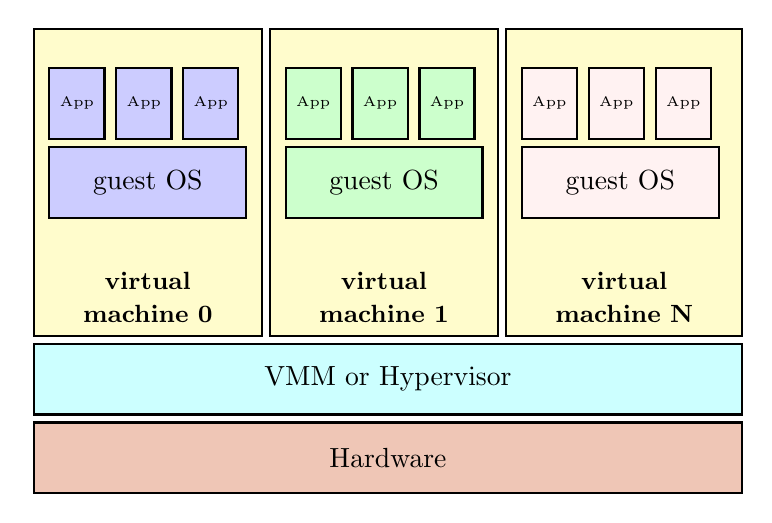
\begin{tikzpicture}

\node at (0,2) [rectangle, draw=black, thick, fill=yellow!20, minimum height = 3.9cm, minimum width = 2.9cm, anchor=south west] (vm0) {};
\node [above, inner sep=5pt, align=center, text width=2.7cm] at (vm0.south) {\textbf{\small{virtual\\ machine 0}}};

\node at (0.2,3.5) [rectangle, draw=black, thick, fill=blue!20, minimum height = 0.9cm, minimum width = 2.5cm, anchor=south west] (g0) {guest OS};
\node at (0.2,4.5) [rectangle, draw=black, thick, fill=blue!20, minimum height = 0.9cm, minimum width = 0.7cm, anchor=south west] (g0app0) {\tiny{App}};
\node at (0.2+0.85,4.5) [rectangle, draw=black, thick, fill=blue!20, minimum height = 0.9cm, minimum width = 0.7cm, anchor=south west] (g0app1) {\tiny{App}};
\node at (0.2+1.7,4.5) [rectangle, draw=black, thick, fill=blue!20, minimum height = 0.9cm, minimum width = 0.7cm, anchor=south west] (g0appn) {\tiny{App}};

\node at (3,2) [rectangle, draw=black, thick, fill=yellow!20, minimum height = 3.9cm, minimum width = 2.9cm, anchor=south west] (vm1) {};
\node [above, inner sep=5pt, align=center, text width=2.7cm] at (vm1.south) {\textbf{\small{virtual\\ machine 1}}};
\node at (3.2,3.5) [rectangle, draw=black, thick, fill=green!20, minimum height = 0.9cm, minimum width = 2.5cm, anchor=south west] (g1) {guest OS};
\node at (3.2,4.5) [rectangle, draw=black, thick, fill=green!20, minimum height = 0.9cm, minimum width = 0.7cm, anchor=south west] (g1app0) {\tiny{App}};
\node at (3.2+0.85,4.5) [rectangle, draw=black, thick, fill=green!20, minimum height = 0.9cm, minimum width = 0.7cm, anchor=south west] (g1app1) {\tiny{App}};
\node at (3.2+1.7,4.5) [rectangle, draw=black, thick, fill=green!20, minimum height = 0.9cm, minimum width = 0.7cm, anchor=south west] (g1appn) {\tiny{App}};

\node at (6,2) [rectangle, draw=black, thick, fill=yellow!20, minimum height = 3.9cm, minimum width = 3cm, anchor=south west] (vmn) {};
\node [above, inner sep=5pt, align=center, text width=2.7cm] at (vmn.south) {\textbf{\small{virtual\\ machine N}}};
\node at (6.2,3.5) [rectangle, draw=black, thick, fill=pink!20, minimum height = 0.9cm, minimum width = 2.5cm, anchor=south west] (gn) {guest OS};
\node at (6.2,4.5) [rectangle, draw=black, thick, fill=pink!20, minimum height = 0.9cm, minimum width = 0.7cm, anchor=south west] (gnapp0) {\tiny{App}};
\node at (6.2+0.85,4.5) [rectangle, draw=black, thick, fill=pink!20, minimum height = 0.9cm, minimum width = 0.7cm, anchor=south west] (gnapp1) {\tiny{App}};
\node at (6.2+1.7,4.5) [rectangle, draw=black, thick, fill=pink!20, minimum height = 0.9cm, minimum width = 0.7cm, anchor=south west] (gnappn) {\tiny{App}};

\node at (0,1) [rectangle, draw=black, thick, fill=Cyan!20, minimum height = 0.9cm, minimum width = 9cm, anchor=south west] (hyper) {VMM or Hypervisor};
\node at (0,0) [rectangle, draw=black, thick, fill=BrickRed!20, minimum height = 0.9cm, minimum width = 9cm, anchor=south west] (hard) {Hardware};


\end{tikzpicture}
\end{center}
\ifreport
\caption{Virtualization Technology}
\fi
\label{fig-virtualization}
\end{figure}



Virtualization has been around for decades. In 1972 IBM released VM/370 operating system for mainframe computers capable of running guest operating systems.
Hypervisor can be classified into two types.
Type-I hypervisor runs bare-metal and has full control over the hardware resources.
An example of type-I hypervisor is Xen \cite{Barham:2003:XAV:1165389.945462}.
Type-II hypervisor runs in a hosted environment on top of another operating system as a process.
An example of type-I hypervisor is KVM \cite{kivity2007kvm}.
The type-II hypervisor can only utilize resources allocated by the host operating system.
Type-I hypervisor can be more efficient than type-II, as it runs directly on the hardware.

\subsection{Virtualization Techniques}
Virtualization can be achieved in number of ways. This section presents well known techniques used for virtualization.

\subsubsection{Classical Virtualization}
In 1974, Popek and Golberg defined virtual machine as \emph{"an efficient, isolated duplicate of the real machine"} and presented formal requirements to virtualize a computer architecture \cite{popek1974formal}. They described three most important characteristics of a virtual machine as follows:

\begin {itemize}
	\item {\textbf{Equivalence:}} The virtual environment provided to the virtual machine is essentially identical. The guest operating system can run in the virtual environment as if running on actual hardware.
	\item {\textbf{Performance:}} The virtual machine running in a virtual environment has comparable performance to when running natively.
	\item {\textbf{Resource Control:}} The virtual machine monitor software is in full control of all the system resources. The guest running in virtual environment has access to only the resources explicitly allocated to this virtual machine.
\end {itemize}

These characteristics provided formal requirements for virtual machine monitor and underlying hardware architecture.
The virtual machine monitor provides duplicate execution environment to the real machine and does not add too much overhead to the execution of virtual machine.
Furthermore, virtual machine monitor has full control over hardware resources.

An instruction set architecture (ISA) of a CPU defines at least two privilege levels or modes of operation.
The set of instructions that can only be executed in highest privileged mode are called \emph{"privileged instructions"}.
Such instruction generate a fault if executed in user mode.
The highest privilege mode is used by operating system kernel to access and manage system resources.
User application run in less privileged mode than the operating system kernel.
Popek and Golberg designated set of instruction that have different behavior depending on the mode of operation as \emph{"sensitive instructions"}.
These instructions included IO operations and instructions that interact with MMU.
Popek and Golberg stated that a computer architecture is virtualizable only if set of sensitive instructions is a subset of privileged instructions. 
The computer architectures that fulfill Popek and Goldberg's criteria are called classically virtualizable architectures.
Classically virtualizable architectures can be used to implement faithful virtualization.
Faithful virtualization technique does not require modification in the guest operating system.

\begin{figure}[!htb]
\begin{center}
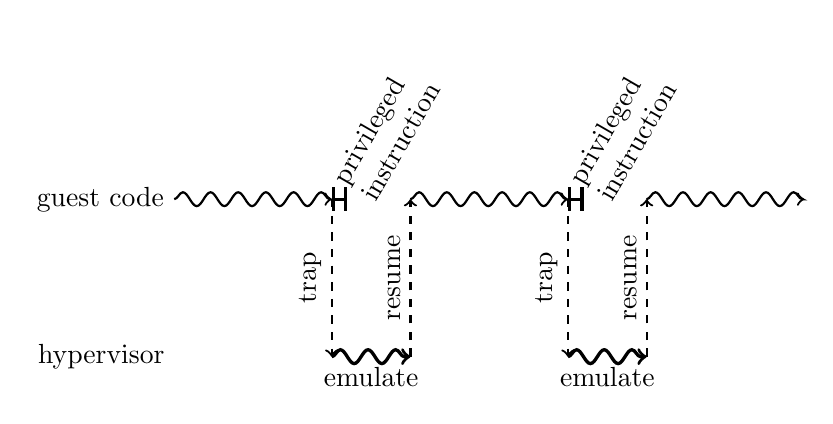
\begin{tikzpicture}


\draw[thick, decorate, decoration=snake, ->] (0, 2) -- (2, 2) node at (0,2) [left] {guest code};
\draw[very thick, |-|] (2, 2) -- (2.2, 2) node [above, right, rotate=60, text width=2cm]{privileged instruction};

\node at (0,0) [left] {hypervisor};
\draw[thick, dashed, ->] (2, 2) -- (2, 0) node [above, align=center,midway, rotate=90]{trap};
\draw[very thick, decorate, decoration=snake, ->] (2.0, 0) -- (3, 0) node [below,midway] {emulate};
\draw[thick, dashed, ->] (3, 0) -- (3, 2) node [above, align=center, midway, rotate=90] {resume};

\draw[thick, decorate, decoration=snake, ->] (3, 2) -- (5, 2);
\draw[very thick, |-|] (5, 2) -- (5.2, 2) node [above, right, rotate=60, text width=2cm]{privileged instruction};

\draw[thick, dashed, ->] (5, 2) -- (5, 0) node [above, align=center,midway, rotate=90]{trap};
\draw[very thick, decorate, decoration=snake, ->] (5, 0) -- (6, 0)  node [below,midway] {emulate};
\draw[thick, dashed, ->] (6, 0) -- (6, 2) node [above, align=center,midway, rotate=90]{resume};

\draw[thick, decorate, decoration=snake, ->] (6, 2) -- (8, 2);

\end{tikzpicture}
\end{center}
\ifreport
\caption{Faithful Virtualization (trap-and-emualte)}
\fi
\label{fig-virt-faithful}
\end{figure}


Faithful virtualization technique allows direct execution of most of the guest code. 
Hypervisor emulates parts of guest code that cannot be executed directly on the hardware.
Faithful virtualization is achieved by executing guest code in a less privileged processor mode in which privileged instruction are not allowed to execute. 
When the processor encounters a privileged instruction it generates a fault, trapping into hypervisor code.
The hypervisor take control and emulates the behavior for faulted guest operating system code. 
Once the required behavior is emulated, guest code starts executing again directly on the CPU.
Figure \ref{fig-virt-faithful} demonstrates faithful virtualization technique.
The guest OS is fooled into believing that it is executing in highest privileged mode.  
This technique is also called trap-and-emulate as virtualization is achieved by emulating trapped guest OS code.   
Faithful virtualization achieves good performance as most of the guest code executes directly. 
%%Unlike paravirtualization in faithful virtualization the guest OS can execute without modification.
%%This technique is also called classical virtualization because the underlying cpu architecture has to satisfy Popek and Goberg requirement for virtualization.


\subsubsection{Software-based Virtualization}
Software-based virtualization technique translates guest operating system instructions into instruction of the target hardware.
It technique is also known as Emulation. 
In this technique behavior of guest OS code is generated by emulating the behavior of guest code. 
Figure \ref{fig-virt-software} demonstrates software-based virtualization technique.
One of the advantages of using emulation is that guest ISA and host ISA can be different. 
Emulation is useful in situations where target hardware is not accessible or very expensive to use. 
\begin{figure}[!htb]
\begin{center}
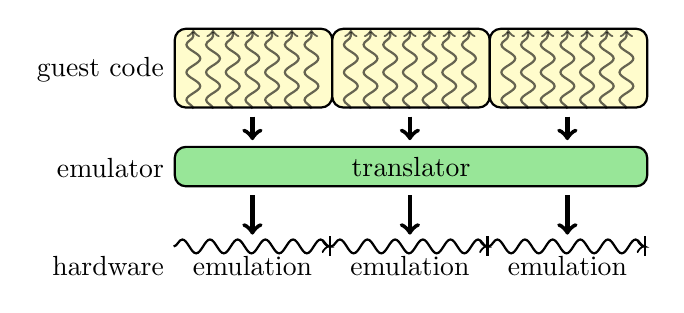
\begin{tikzpicture}

\node at (0,2.5) [left] {guest code};
\node at (0,2) [rectangle, draw=black, thick, rounded corners, fill=yellow!20,  minimum height = 1cm, minimum width = 2cm, anchor=south west] (b1) {};
\begin {scope} [opacity=0.6]
\draw[thick, decorate, decoration=snake, ->] (0.25, 2) -- (0.25, 3);
\draw[thick, decorate, decoration=snake, ->] (0.5, 2) -- (0.5, 3);
\draw[thick, decorate, decoration=snake, ->] (0.75, 2) -- (0.75, 3);
\draw[thick, decorate, decoration=snake, ->] (1, 2) -- (1, 3);
\draw[thick, decorate, decoration=snake, ->] (1.25, 2) -- (1.25, 3);
\draw[thick, decorate, decoration=snake, ->] (1.5, 2) -- (1.5, 3);
\draw[thick, decorate, decoration=snake, ->] (1.75, 2) -- (1.75, 3);
\end {scope}

\node at (2,2) [rectangle, draw=black, thick, rounded corners, fill=yellow!20, minimum height = 1cm, minimum width = 2cm, anchor=south west] (b2) {};
\begin {scope} [opacity=0.6]
\draw[thick, decorate, decoration=snake, ->] (2.25, 2) -- (2.25, 3);
\draw[thick, decorate, decoration=snake, ->] (2.5, 2) -- (2.5, 3);
\draw[thick, decorate, decoration=snake, ->] (2.75, 2) -- (2.75, 3);
\draw[thick, decorate, decoration=snake, ->] (3, 2) -- (3, 3);
\draw[thick, decorate, decoration=snake, ->] (3.25, 2) -- (3.25, 3);
\draw[thick, decorate, decoration=snake, ->] (3.5, 2) -- (3.5, 3);
\draw[thick, decorate, decoration=snake, ->] (3.75, 2) -- (3.75, 3);
\end {scope}

\node at (4,2) [rectangle, draw=black, thick, rounded corners, fill=yellow!20, minimum height = 1cm, minimum width = 2cm, anchor=south west] (b2) {};
\begin {scope} [opacity=0.6]
\draw[thick, decorate, decoration=snake, ->] (4.25, 2) -- (4.25, 3);
\draw[thick, decorate, decoration=snake, ->] (4.5, 2) -- (4.5, 3);
\draw[thick, decorate, decoration=snake, ->] (4.75, 2) -- (4.75, 3);
\draw[thick, decorate, decoration=snake, ->] (5, 2) -- (5, 3);
\draw[thick, decorate, decoration=snake, ->] (5.25, 2) -- (5.25, 3);
\draw[thick, decorate, decoration=snake, ->] (5.5, 2) -- (5.5, 3);
\draw[thick, decorate, decoration=snake, ->] (5.75, 2) -- (5.75, 3);
\end {scope}

\draw[ultra thick, ->] (1, 1.9) -- (1, 1.6);
\draw[ultra thick, ->] (3, 1.9) -- (3, 1.6);
\draw[ultra thick, ->] (5, 1.9) -- (5, 1.6);
\draw[ultra thick, ->] (1, 0.9) -- (1, 0.4);
\draw[ultra thick, ->] (3, 0.9) -- (3, 0.4);
\draw[ultra thick, ->] (5, 0.9) -- (5, 0.4);

\node at (0,1) [rectangle, draw=black, thick, rounded corners,  fill=LimeGreen!50, minimum height = 0.5cm, minimum width = 6cm, anchor=south west] (tr) {translator};
\node at (0,1.25) [left] {emulator};

\node at (0,0) [left] {hardware};
\draw[thick, decorate, decoration=snake, ->|] (0, 0.25) -- (2, 0.25)  node [below, align=center, midway, text width=2cm] {emulation};
\draw[thick, decorate, decoration=snake, ->|] (2, 0.25) -- (4, 0.25)  node [below, align=center, midway, text width=2cm] {emulation};
\draw[thick, decorate, decoration=snake, ->|] (4, 0.25) -- (6, 0.25)  node [below, align=center, midway, text width=2cm] {emulation};

\end{tikzpicture}
\end{center}
\ifreport
\caption{Software-based Virtualization}
\fi
\label{fig-virt-software}
\end{figure}


The performance of emulation is poor compared to other virtualization techniques where guest code can run directly on the target hardware. 
Techniques like dynamic binary translation and translation cache are used to improve the performance of an emulator \cite{ebcioglu2001dynamic}.
An example of virtualization software from this class is QEMU \cite{bellard2005qemu}.
QEMU is one of the most extensively used emulator, it uses optimization techniques like binary translation and translation cache to improve performance. 
%%A very simple mechnism of virtualization is to emulate the guest OS instruction behavior.

\subsubsection{Paravirtualization}
%Classical virtualization requires underlying hardware to trap guest operating system for all sensitive instrucitons. If architecture
Paravirtualization is a technique in which the hypervisor provides set of functions to the guest operating system to perform sensitive operations. 
The guest operating system is modified to replace sensitive instruction with function calls, also referred as hypercalls.
The guest operating system software is executed directly on the hardware as long as no sensitive operation is required. 
Figure \ref{fig-virt-para} demonstrates paravirtualization technique.
A disadvantage of this technique is that guest OS has to be modified to to replace sensitive operations.
\begin{figure}[!htb]
\begin{center}
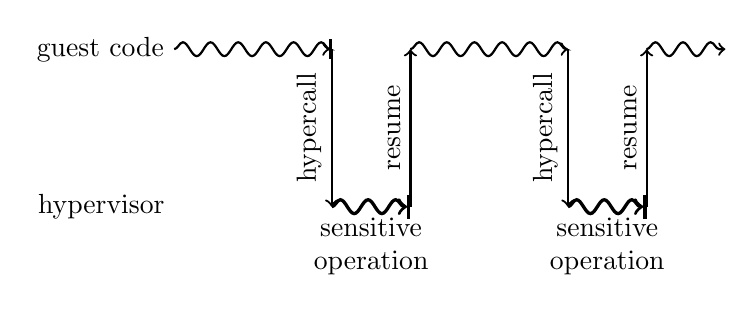
\begin{tikzpicture}


\draw[thick, decorate, decoration=snake, ->|] (0, 2) -- (2, 2) node at (0,2) [left] {guest code};
%\draw[thick, |-|] (2, 2) -- (2.3, 2) ; node [right, rotate=90, text width=2cm]{sensitive instruction};

\node at (0,0) [left] {hypervisor};
\draw[thick, ->] (2, 2) -- (2, 0) node [above, align=center,midway, rotate=90]{hypercall};
\draw[very thick, decorate, decoration=snake, ->|] (2.0, 0) -- (3, 0)   node [below, align=center, midway, text width=2cm] {sensitive operation};
\draw[thick, ->] (3, 0) -- (3, 2) node [above, align=center, midway, rotate=90] {resume};

\draw[thick, decorate, decoration=snake, ->] (3, 2) -- (5, 2);
%\draw[thick, |-|] (5, 2) -- (5.3, 2) node [right, rotate=90, text width=2cm]{sensitive operation};

\draw[thick, ->] (5, 2) -- (5, 0) node [above, align=center,midway, rotate=90]{hypercall};
\draw[very thick, decorate, decoration=snake, ->|] (5, 0) -- (6, 0)  node [below, align=center, midway, text width=2cm] {sensitive operation};
\draw[thick, ->] (6, 0) -- (6, 2) node [above, align=center,midway, rotate=90]{resume};

\draw[thick, decorate, decoration=snake, ->] (6, 2) -- (7, 2);

\end{tikzpicture}
\end{center}
\ifreport
\caption{Paravirtualization}
\fi
\label{fig-virt-para}
\end{figure}


The performance of paravirtualized guest OS is very close to executing guest operating system bare-metal.
An advantage of using paravirtualization over faithful virtualization is it can be used for architectures that lack hardware support for virtualization.
An example from this class is Xen hypervisor \cite{Barham:2003:XAV:1165389.945462}.
Xen is type-1 hypervisor that initially used paravirtualization to virtualize architectures that are not virtualizable. 
Xen also supports faithful virtualization through hardware-assisted virtualization.

\subsection{Virtualization of Real-time Applications}

Virtualization has been around for decades however the main area of deployment was usually desktop and server computers.
Since real-time system are subjected to strict timing constraints and require deterministic response times, any virtualization solution for real-time applications must address these issues.
Over the past few years many virtualization solutions for real-time applications has been proposed.
Most virtualization solutions are customized to target one or a set of similar market segments of real-time systems. 
An example is Xtratum hypervisor which is specifically designed to host safety critical applications \cite{Carrascosa:2014:XHR:2668138.2668142}.
Custom designed commercial virtualization solutions for real-time application also exist. 
Examples include WindRiver hypervisor for VxWorks \cite{bialowas2010achieving}, 
Greenhills INTEGRITY multivisor\cite{greenhills-multivisor}, 
Real-Time Systems GmbH Hypervisor \cite{realtime-systems-gmbh-hypervisor}
SysGO PikeOS \cite{kaiser2007pikeos}, 
and National Instruments Real-Time Hypervisor \cite{ni-realtime-hypervisor}.

Many researchers has focused on bringing real-time capabilities to widely used open-source virtualization software.
Xen \cite{Barham:2003:XAV:1165389.945462} is an open-source type-1 hypervisor widely used in research and cloud services.
A large amount of research has been conducted to make is acceptable for real-time applications.
Masrur et al. \cite{masrur2010vm} evaluated real-time performance of Xen SEDF (Simple Earliest Deadline First)
scheduling algorithm. They proposed PSEDF (Priority-based scheduling plus SEDF) that separates
real-time domains from other domains to achieve lower latencies and jitter.
RT-Xen project \cite{Xi:2011:RTR:2038642.2038651} has developed real-time scheduling framework for Xen.
Xen uses split-driver architecture for handling I/O. A special guest, called domain0, contains the
back-end driver and other guests (referred as user domains) contain front-end driver.
Physical interrupts are first delivered to hypervisor. Hypervisor passes them to back-end drivers in domain0.
From domain0 they are routed to the front-end drivers in user domains.
Many research efforts has been made to lower interrupt response times caused by split-driver model.

KVM on the other hand is a type-2 hypervisor and uses Linux as host \cite{kivity2007kvm}. 
It is also an open-source project and extensively used in virtualization solution for enterprise domain.
Kiszka \cite{kiszka2009towards} proposed real-time improvements to Linux host to append real-time capabilities to KVM.
One of the improvements was using PREEMPT\_RT patch to append real-time capabilities to host Linux kernel.
Zhang et al. \cite{zuo2010performance} proposed real-time virtualization solution based on KVM and suggested improvements to 
enhance real-time performance. The improvements include CPU shielding and interrupt prioritization. CPU shiedling
refers to allocating a CPU core to real-time application. 

Many real-time virtualization solutions based on L4 microkernel has been proposed. 
In contrast to monolithic kernel, microkernel based designs enjoys the benefit of having small TCB \cite{Heiser:2008:RVE:1435458.1435461}.
Examples include OKL4 microkernel-based hypervisor designed by Open Kernel Labs and PikeOS hypervisor developed by SysGo.
One application area for microkernel-based virtualization solutions is mobile platforms like smart phones.
The light weight virtualization solution can enable co-existence of a GPOS for user interface applications and
RTOS to handle performance critical tasks.

%%Aavailability of large amounts of computational power on a single multicore chip and emerging technological trends has brought new opportunities and challenges for real-time systems.
%%Virtualization can be used to consolidate mixed criticality applications to efficiently use computational resources on multicore chip and reduced system costs.
%%Real-time systems are now accessible than ever before. Emerging technological trends has streered them to provide user access over the network.
%%Virtualization can provide security to real-time applications.
%%Many real-time applications run on a hetrogeneous computing platform with non real-time applications running aside. 
%%Virtualization can be used in such scenarios to isolated real-time applications from others.

\subsection{Virtual Machines on Multicore}
Multicore processors has become a norm and the average number of cores available per processors are expected to increase in future.
Multicore processing provides unique opportunities for real-time virtualization solutions.
Multicore processors has enabled co-location of applications of mixed-criticality on one platform by sandboxing each on separate set of cores.
Real-time applications can be assigned a dedicated processor core(s) to ensure spatial isolation from other applications.
It enables consolidation of application of mixed-criticality on one machine that reduces system cost.
Many virtualization solutions has been proposed that use separate CPU cores to isolate real-time applications
from others. Examples include Quest-V \cite{West:2016:VSK:2966277.2935748} and Xtratum \cite {Carrascosa:2014:XHR:2668138.2668142} hypervisors.


\section{Hardware-Assisted Virtualization on x86}
For a long time, the x86 architecture was not virtualizable as it did not fulfill Popek and Goldberg's criteria.
Software-based emulation has remained the only choice of faithful virtualization for x86 architecture until 2005.
In year 2005, Intel \cite{uhlig2005intel} and AMD released hardware extensions (VT-x and SVM respectively) that allowed x86 to be virtualized using classical trap-and-emulate technique.
This section presents how hardware-assisted virtualization works.
The discussion is primarily based on Intel VT-x technology however it is equally valid for AMD SVM.

\subsection{Processor Operation Modes}
Intel Virtualization Technology (VT-x) adds virtual machine extensions (VMX) to existing x86 architecture.
The technology defines two new modes of processor operation: VMX root operation mode and VMX non-root operation mode \cite{intel-sdm-vol3}.
%The hypervisor runs in VMX root operation which is highest priviledge mode, and guest operation system executes in VMX non-root operation which is less privileged than VMX root operation mode.
The hypervisor runs in VMX root operation mode and guest operating system executes in VMX non-root operation mode.
Both modes of operation include all privilege rings, which allows guest code to run at its intended ring. 
Hence no de-privileging is needed for the guest OS.

VT-x technology defines two types of transition for VMX operation modes. 
Transition into VMX non-root operation are called VM entries. 
Transition from VMX non-root to VMX root operation mode are called VM exits.
In VMX root operation mode processor functionality is extended with new instruction set that
hypervisor can use to create and manage virtual machines.
%The functionality of VMX root operation is same as if processor is executing in kernel mode, except that there are new instructions defined for hypervisor manage virtual machines. 
The functionality of VMX non-root operation is restricted. 
Execution of a sensitive instruction can cause VM exit giving control back to hypervisor.
Once virtual machine is properly configured by the hypervisor, these modes of operation are hidden from the guest. 

\subsection{Virtual Machine Control Structure}
VT-x technology allows configuration and management of a virtual machine via data structure called virtual machine control structure (VMCS).
The hypervisor can control behavior of virtual CPU by properly configuring VMCS data structure.
Hypervisor is responsible to allocate, initialize and manage one VMCS data structure for each virtual processor.
The VMCS is further divided into subfields as follows:
\begin{itemize}
	\item \textbf{Guest-state area} used to load and store guest state on vmx transitions
	\item \textbf{Host-state area} used to load and store host state on vmx transitions
	\item \textbf{VM-execution control fields} includes fields to controls vmx non-root operation mode
	\item \textbf{VM-exit control fields} includes fields to controls vmexit transition
	\item \textbf{VM-entry control fields} includes fields to control vmentry transition
	\item \textbf{VM-exit information fields} used to store information about vmexit transition
\end{itemize}

VT-x technology supports new instructions that hypervisor can use in VMX root operating mode to manage VMCS.
For example to read and write a field of VMCS host uses VMREAD and VMWRITE instruction respectively.

\begin{figure}[!htb]
\begin{center}
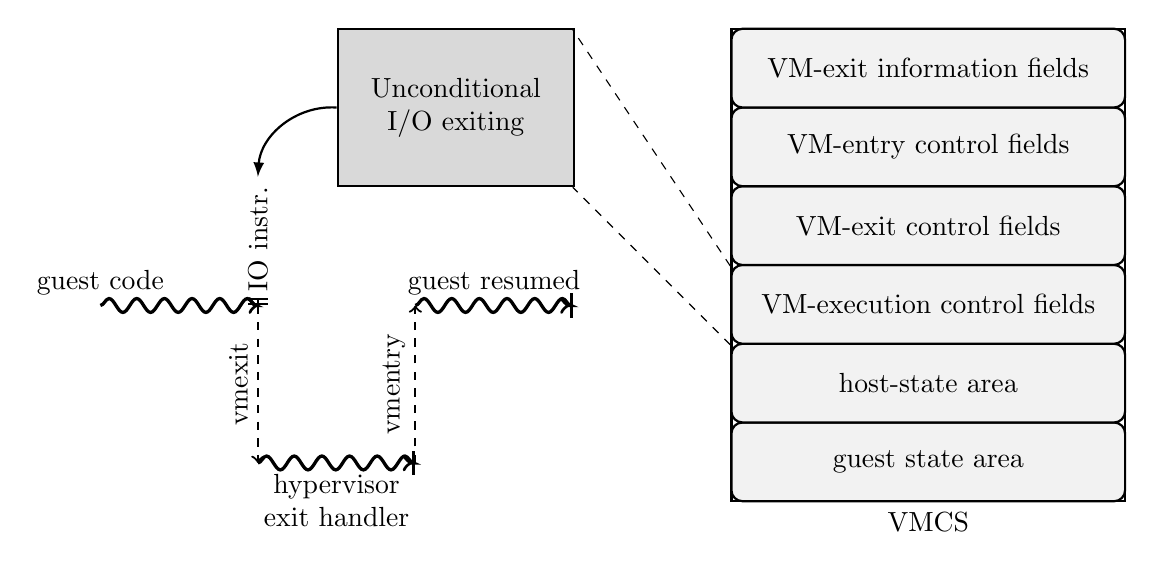
\begin{tikzpicture}

%\draw[step=0.5cm, gray, very thin] (0,0) grid (9,9)


\draw[very thick, decorate, decoration=snake, ->] (0, 2.5) -- (2, 2.5) node at (0,2.5) [above] {guest code};
\draw[thick, |-|] (2, 2.5) -- (2, 2.6) node at (2, 2.6)[right, midway, rotate=90] (ioinst) {IO instr.};

\draw[very thick, decorate, decoration=snake, ->|] (2, 0.5) -- (4, 0.5) node [below, midway, align=center] {hypervisor\\ exit handler};
\draw[very thick, decorate, decoration=snake, ->|] (4, 2.5) -- (6, 2.5) node [above, align=center, midway] {guest resumed};

\draw[thick, dashed, ->] (2, 2.5) -- (2, 0.5) node [above, align=center,midway, rotate=90] {vmexit};
\draw[thick, dashed, ->] (4, 0.5) -- (4, 2.5) node [above, align=center,midway, rotate=90] {vmentry};


\node at (3,4) [rectangle, draw=black, thick, fill=black!15, minimum height = 2cm, minimum width = 3cm, anchor=south west, align=center] (exitcontrol) 
                        {Unconditional\\ I/O exiting} ;


\node at (8,0) [rectangle, draw=black, thick, fill=white, minimum height = 6cm, minimum width = 5cm, anchor=south west] (vmcs) {} ;
\node [below, align=center] at (vmcs.south) {VMCS};
%\node[below right, inner sep=5pt, text width=2cm] at (rtguest.north west) {PREEMPT\_RT\\ Linux\\ (rt-guest)};


\node at (8,0) [rectangle, draw=black, thick, rounded corners, fill=black!5, minimum height = 1cm, minimum width = 5cm, anchor=south west] (gstate) {guest state area};
\node at (8,1) [rectangle, draw=black, thick, rounded corners, fill=black!5, minimum height = 1cm, minimum width = 5cm, anchor=south west] (gstate) {host-state area};
\node at (8,2) [rectangle, draw=black, thick, rounded corners, fill=black!5, minimum height = 1cm, minimum width = 5cm, anchor=south west] (gstate) {VM-execution control fields};
\node at (8,3) [rectangle, draw=black, thick, rounded corners, fill=black!5, minimum height = 1cm, minimum width = 5cm, anchor=south west] (gstate) {VM-exit control fields};
\node at (8,4) [rectangle, draw=black, thick, rounded corners, fill=black!5, minimum height = 1cm, minimum width = 5cm, anchor=south west] (gstate) {VM-entry control fields};
\node at (8,5) [rectangle, draw=black, thick, rounded corners, fill=black!5, minimum height = 1cm, minimum width = 5cm, anchor=south west] (gstate) {VM-exit information fields};

\draw [dashed] (8,2) -- (6,4); 
\draw [dashed] (8,3) -- (6,6); 

\begin{scope}[>=latex]
	\draw [thick, ->] (exitcontrol.west) to [bend right=45] (ioinst.east);
\end{scope}

\end{tikzpicture}
\end{center}
\ifreport
\caption{VMCS data structure with an example of using VMCS fields to control guest execution behavior}
\fi
\label{fig-vmcs-ds}
\end{figure}


\subsection{Virtual Machine Control Flow}
The hypervisor enters VMX root operation mode by executing VMXON instruction.
VMLAUNCH instruction is used to launch a virtual machine that causes VM entry.
On VM entry transition hardware loads guest state from the guest-state area of VMCS
and begins execution of guest code at an address specified in VMCS.
During VM entry transition the hardware checks fields of VMCS to 
identify if hypervisor has request injection of a virtual interrupt.
If so, the virtual interrupt is delivered to the guest right after VM entry transition.
Flags in VMCS VM-execution control fields area define when to take VM exit transition.
For example \emph{"Unconditional IO exiting"} flag with cause VM exit transition 
when guest code tries to execute an IO instruction. Figure \ref{fig-vmcs-ds} demonstrates 
what happens when IO instruction is encountered in guest code.
Similarly \emph{"external interrupt exiting"} will cause VM exit transition if
an external interrupt arrives in vmx non-root operation mode, giving control back to hypervisor.
During VM exit transition the hardware stores guest state back to guest-state area in VMCS and
loads host state from host-state area in VMCS.
Furthermore, the detailed information about the cause of VM exit transition is
saved in VM-exit information area in VMCS. This information helps hypervisor
to determine appropriate action required to emulate guest behavior.

\subsection{Features for Efficient Virtualization}
This section sheds light upon x86 hardware features that enable efficient virtualization of guests.

\subsubsection{MMU Virtualization} \label{sec:vmmu}
In a virtualized environment a guest executes in its own virtual address space and hypervisor has full control over the physical memory.
In order to keep the illusion that guest has control over physical memory, hypervisor uses nested page-tables also known as shadow page-tables.
When a guest tries to access physical memory, guest physical addresses are treated as virtual addresses and 
translated to real physical addresses through nested page-tables.
The nested page-tables can be implemented in software in which case software emulates the behavior of page-table walk to
translate guest physical address (host virtual address) to host physical addresses.

\begin{figure}[!htb]
\begin{center}
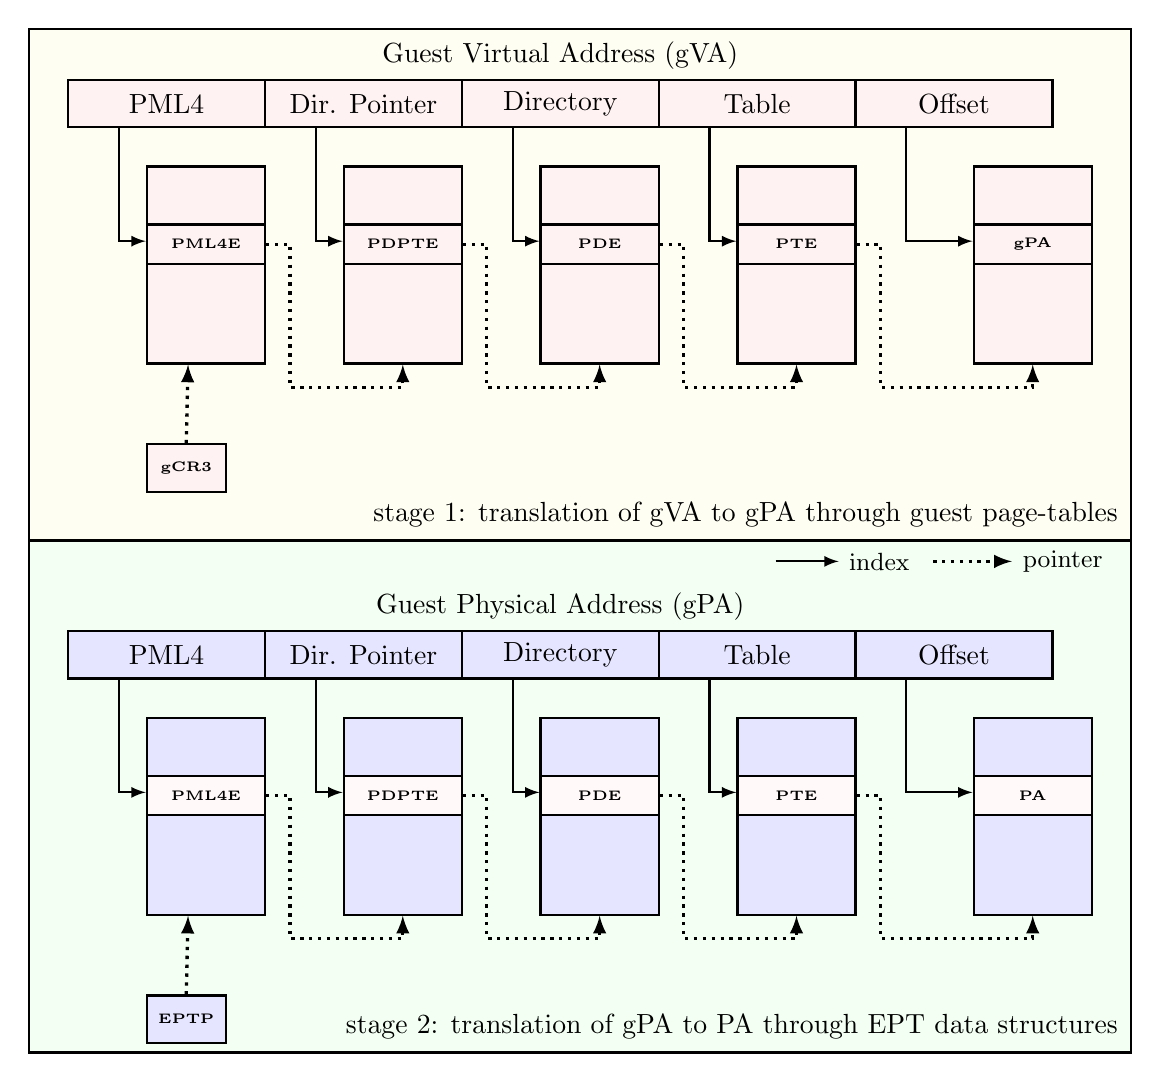
\begin{tikzpicture}

\node at (-0.5,-5-0.25) [rectangle, draw=black, thick, fill=yellow!5, minimum height = 6.5cm, minimum width = 14cm, anchor=south west] (stage1) {};
\node [above left, inner sep=5pt] at (stage1.south east) {\textbf\small{{stage 1: translation of gVA to gPA through guest page-tables}}};

\node at (0,0) [rectangle, draw=black, thick, fill=pink!20, minimum height = 0.6cm, minimum width = 2.5cm, anchor=south west] (gpml4) {PML4};
\node at (0+2.5,0) [rectangle, draw=black, thick, fill=pink!20, minimum height = 0.6cm, minimum width = 2.5cm, anchor=south west] (gdirptr) {Dir. Pointer};
\node at (0+2.5+2.5,0) [rectangle, draw=black, thick, fill=pink!20, minimum height = 0.6cm, minimum width = 2.5cm, anchor=south west] (gdir) {Directory};
\node [above, align=center] at (gdir.north) {\textbf\small{{Guest Virtual Address (gVA)}}};
\node at (0+2.5+2.5+2.5,0) [rectangle, draw=black, thick, fill=pink!20, minimum height = 0.6cm, minimum width = 2.5cm, anchor=south west] (gtbl) {Table};
\node at (0+2.5+2.5+2.5+2.5,0) [rectangle, draw=black, thick, fill=pink!20, minimum height = 0.6cm, minimum width = 2.5cm, anchor=south west] (goff) {Offset};


\node at (1.0,-3) [rectangle, draw=black, thick, fill=pink!20, minimum height = 2.5cm, minimum width = 1.5cm, anchor=south west] (gpgpml4) {};
\node [rectangle, draw=black, thick, fill=pink!20, minimum height = 0.5cm, minimum width = 1.5cm, anchor=south west] at (gpgpml4.west) (gpgpml4e) 
				{\tiny\textbf{{PML4E}}};

\node at (1.0,-4)  [rectangle, draw=black, thick, fill=pink!20, minimum height = 0.6cm, minimum width = 1.0cm, anchor=north west] (gcr3) 
				{\tiny\textbf{{gCR3}}};

\node at (3.5,-3) [rectangle, draw=black, thick, fill=pink!20, minimum height = 2.5cm, minimum width = 1.5cm, anchor=south west] (gpgdirptr) {};
\node [rectangle, draw=black, thick, fill=pink!20, minimum height = 0.5cm, minimum width = 1.5cm, anchor=south west] at (gpgdirptr.west) 
			    (gpgdirptre) {\tiny\textbf{{PDPTE}}};
\node at (6,-3) [rectangle, draw=black, thick, fill=pink!20, minimum height = 2.5cm, minimum width = 1.5cm, anchor=south west] (gpgdir) {};
\node [rectangle, draw=black, thick, fill=pink!20, minimum height = 0.5cm, minimum width = 1.5cm, anchor=south west] at (gpgdir.west) 
                (gpgdire) {\tiny\textbf{{PDE}}};
\node at (8.5,-3) [rectangle, draw=black, thick, fill=pink!20, minimum height = 2.5cm, minimum width = 1.5cm, anchor=south west] (gpgtbl) {};
\node [rectangle, draw=black, thick, fill=pink!20, minimum height = 0.5cm, minimum width = 1.5cm, anchor=south west] at (gpgtbl.west) 
                (gpgtble) {\tiny\textbf{{PTE}}};
\node at (11.5,-3) [rectangle, draw=black, thick, fill=pink!20, minimum height = 2.5cm, minimum width = 1.5cm, anchor=south west] (gpgoff) {};
\node [rectangle, draw=black, thick, fill=pink!20, minimum height = 0.5cm, minimum width = 1.5cm, anchor=south west] at (gpgoff.west) 
                {\tiny\textbf{{gPA}}};


\begin{scope}[>=latex]	
	\draw [thick, ->] ([xshift=-4ex]gpml4.south) |- ([yshift=2ex]gpgpml4.west);
	\draw [thick, ->] ([xshift=-4ex]gdirptr.south) |- ([yshift=2ex]gpgdirptr.west);
	\draw [thick, ->] ([xshift=-4ex]gdir.south) |- ([yshift=2ex]gpgdir.west);
	\draw [thick, ->] ([xshift=-4ex]gtbl.south) |- ([yshift=2ex]gpgtbl.west);
	\draw [thick, ->] ([xshift=-4ex]goff.south) |- ([yshift=2ex]gpgoff.west);

	%\draw [thick, dotted, ->] ([yshift=-1ex]gpgpml4e.south) to [bend right=75] (gpgdirptr.south);

	\draw [very thick, dotted, ->] (gcr3.north) -- ([xshift=-1.5ex]gpgpml4.south);
	\draw [very thick, dotted, ->] (gpgpml4e.east) -| ([xshift=2ex]gpgpml4e.east) -- ([xshift=2ex, yshift=-12ex]gpgpml4e.east) -| (gpgdirptr.south);
	\draw [very thick, dotted, ->] (gpgdirptre.east) -| ([xshift=2ex]gpgdirptre.east) -- ([xshift=2ex, yshift=-12ex]gpgdirptre.east) -| (gpgdir.south);
	\draw [very thick, dotted, ->] (gpgdire.east) -| ([xshift=2ex]gpgdire.east) -- ([xshift=2ex, yshift=-12ex]gpgdire.east) -| (gpgtbl.south);
	\draw [very thick, dotted, ->] (gpgtble.east) -| ([xshift=2ex]gpgtble.east) -- ([xshift=2ex, yshift=-12ex]gpgtble.east) -| (gpgoff.south);	

\end{scope}

\node at (-0.5,-5-7+0.25) [rectangle, draw=black, thick, fill=green!5, minimum height = 6.5cm, minimum width = 14cm, anchor=south west] (stage2) {};
\node [above left, inner sep=5pt] at (stage2.south east) {\textbf\small{{stage 2: translation of gPA to PA through EPT data structures}}};

\node at (0,0-7) [rectangle, draw=black, thick, fill=blue!10, minimum height = 0.6cm, minimum width = 2.5cm, anchor=south west] (gpml4) {PML4};
\node at (0+2.5,0-7) [rectangle, draw=black, thick, fill=blue!10, minimum height = 0.6cm, minimum width = 2.5cm, anchor=south west] (gdirptr) {Dir. Pointer};
\node at (0+2.5+2.5,0-7) [rectangle, draw=black, thick, fill=blue!10, minimum height = 0.6cm, minimum width = 2.5cm, anchor=south west] (gdir) {Directory};
\node [above, align=center] at (gdir.north) {\textbf\small{{Guest Physical Address (gPA)}}};
\node at (0+2.5+2.5+2.5,0-7) [rectangle, draw=black, thick, fill=blue!10, minimum height = 0.6cm, minimum width = 2.5cm, anchor=south west] (gtbl) {Table};
\node at (0+2.5+2.5+2.5+2.5,0-7) [rectangle, draw=black, thick, fill=blue!10, minimum height = 0.6cm, minimum width = 2.5cm, anchor=south west] (goff) {Offset};


\node at (1.0,-3-7) [rectangle, draw=black, thick, fill=blue!10, minimum height = 2.5cm, minimum width = 1.5cm, anchor=south west] (gpgpml4) {};
\node [rectangle, draw=black, thick, fill=pink!10, minimum height = 0.5cm, minimum width = 1.5cm, anchor=south west] at (gpgpml4.west) (gpgpml4e) 
				{\tiny\textbf{{PML4E}}};

\node at (1.0,-4-7)  [rectangle, draw=black, thick, fill=blue!10, minimum height = 0.6cm, minimum width = 1.0cm, anchor=north west] (eptp) 
				{\tiny\textbf{{EPTP}}};

\node at (3.5,-3-7) [rectangle, draw=black, thick, fill=blue!10, minimum height = 2.5cm, minimum width = 1.5cm, anchor=south west] (gpgdirptr) {};
\node [rectangle, draw=black, thick, fill=pink!10, minimum height = 0.5cm, minimum width = 1.5cm, anchor=south west] at (gpgdirptr.west) 
			    (gpgdirptre) {\tiny\textbf{{PDPTE}}};
\node at (6,-3-7) [rectangle, draw=black, thick, fill=blue!10, minimum height = 2.5cm, minimum width = 1.5cm, anchor=south west] (gpgdir) {};
\node [rectangle, draw=black, thick, fill=pink!10, minimum height = 0.5cm, minimum width = 1.5cm, anchor=south west] at (gpgdir.west) 
                (gpgdire) {\tiny\textbf{{PDE}}};
\node at (8.5,-3-7) [rectangle, draw=black, thick, fill=blue!10, minimum height = 2.5cm, minimum width = 1.5cm, anchor=south west] (gpgtbl) {};
\node [rectangle, draw=black, thick, fill=pink!10, minimum height = 0.5cm, minimum width = 1.5cm, anchor=south west] at (gpgtbl.west) 
                (gpgtble) {\tiny\textbf{{PTE}}};
\node at (11.5,-3-7) [rectangle, draw=black, thick, fill=blue!10, minimum height = 2.5cm, minimum width = 1.5cm, anchor=south west] (gpgoff) {};
\node [rectangle, draw=black, thick, fill=pink!10, minimum height = 0.5cm, minimum width = 1.5cm, anchor=south west] at (gpgoff.west) 
                {\tiny\textbf{{PA}}};

\begin{scope}[>=latex]	
	\draw [thick, ->] ([xshift=-4ex]gpml4.south) |- ([yshift=2ex]gpgpml4.west);
	\draw [thick, ->] ([xshift=-4ex]gdirptr.south) |- ([yshift=2ex]gpgdirptr.west);
	\draw [thick, ->] ([xshift=-4ex]gdir.south) |- ([yshift=2ex]gpgdir.west);
	\draw [thick, ->] ([xshift=-4ex]gtbl.south) |- ([yshift=2ex]gpgtbl.west);
	\draw [thick, ->] ([xshift=-4ex]goff.south) |- ([yshift=2ex]gpgoff.west);

	\draw [very thick, dotted, ->] (eptp.north) -- ([xshift=-1.5ex]gpgpml4.south);
	\draw [very thick, dotted, ->] (gpgpml4e.east) -| ([xshift=2ex]gpgpml4e.east) -- ([xshift=2ex, yshift=-12ex]gpgpml4e.east) -| (gpgdirptr.south);
	\draw [very thick, dotted, ->] (gpgdirptre.east) -| ([xshift=2ex]gpgdirptre.east) -- ([xshift=2ex, yshift=-12ex]gpgdirptre.east) -| (gpgdir.south);
	\draw [very thick, dotted, ->] (gpgdire.east) -| ([xshift=2ex]gpgdire.east) -- ([xshift=2ex, yshift=-12ex]gpgdire.east) -| (gpgtbl.south);
	\draw [very thick, dotted, ->] (gpgtble.east) -| ([xshift=2ex]gpgtble.east) -- ([xshift=2ex, yshift=-12ex]gpgtble.east) -| (gpgoff.south);	

	\draw [very thick, dotted, ->] (11,-5.5) -- (12, -5.5) node [right] {\small{pointer}};
	\draw [thick, ->] (9,-5.5) -- (9.8, -5.5) node [right] {\small{index}};
\end{scope}

\end{tikzpicture}
\end{center}
\ifreport
\caption{MMU Virtualization}
\fi
\label{fig-vmmu}
\end{figure}


Recent revisions of hardware-assisted virtualization extensions of x86 supports translation of guest physical address to host physical address 
in hardware using feature called extended page-tables (EPT). 
The feature removes the need of maintaining nested page-tables in software, hence reducing software overhead to perform the translation.
Figure \ref{fig-vmmu} shows how guest virtual address is translated to machine physical address using EPT data structures.
The first stage is a usual, the guest virtual address is translated to guest physical address by using guest page-tables.
The guest physical address is then translated in hardware in stage 2 using extended page-tables. The translation processor is
autonomous.

VT-x extensions also added the concept of virtual-processor identifiers (VPIDs). 
The feature allows processor the cache address translation of multiple address spaces by associated different VPIDs to each address space.
VPID is 16-bit identifier assigned to a guest by hypervisor during virtual machine initialization.
This feature also allows VPID based TLB flushing and clearing single translations.

\subsubsection{APIC Virtualization} \label{sec:vapic}
x86 virtualization extensions VT-x supports virtualization of Local APIC (Advanced Programmable Interrupt Controller). 
The APIC virtualization (APIC-v) allows emulation of most interrupt controller register accesses by the guest and keeps track of the virtual APIC state. 
APIC-v supports direct injection of the virtual interrupts without hypervisor intervention through a feature called posted interrupts (PI).
The feature requires hypervisor to allocate a memory page for the guest where virtual state of the APIC is maintained by the hardware.
All read accesses to the APIC registers are emulated in hardware by passing contents of virtual APIC memory page without hypervisor intervention.
The write accesses to APIC registers are also emulated in hardware by writing new values to virtual APIC page. 
However for certain registers hypervisor intervention is required and the control is transferred to hypervisor at end of write emulation.
Figure \ref{fig-vapic} displays how virtual APIC page is accessed by the guest without hypervisor involvement. 
Hypervisor is responsible to allocate virtual APIC page and store address of the page in VMCS before initializing a virtual machine.
From there onwards all access to APIC by the guest are virtualized by hardware.

\begin{figure}[!htb]
\begin{center}
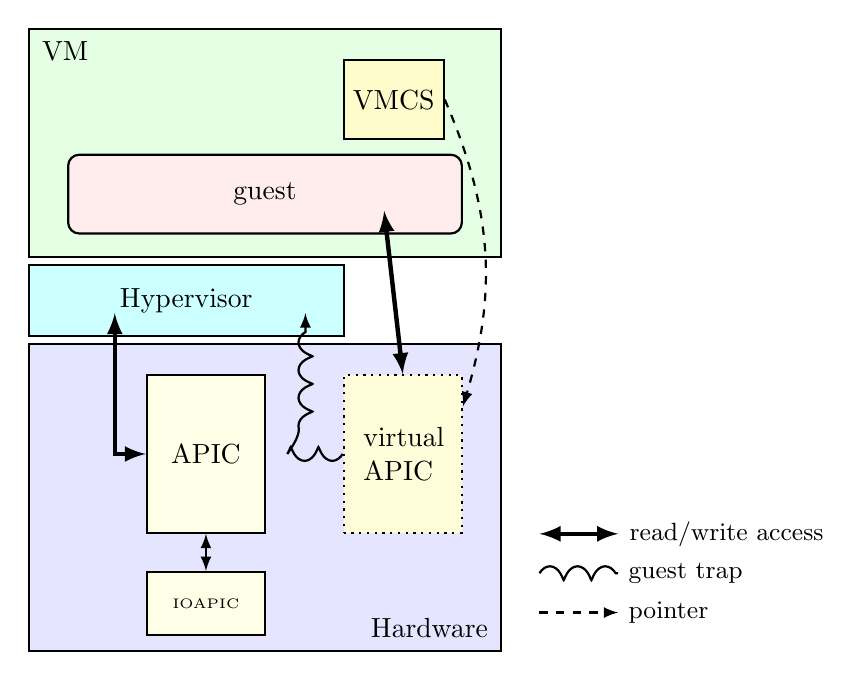
\begin{tikzpicture}

\node at (0,5) [rectangle, draw=black, thick, fill=green!10, minimum height = 2.9cm, minimum width = 6cm, anchor=south west] (vm) {};
\node [below right, inner sep=5pt] at (vm.north west) {VM};

\node at (0.5,5.3) [rectangle, rounded corners, draw=black, thick, fill=pink!30, minimum height = 1cm, minimum width = 5cm, anchor=south west] (g) {guest};
\node at (4.0,6.5) [rectangle, draw=black, thick, fill=yellow!20, minimum height = 1cm, minimum width = 0.5cm, anchor=south west] (vmcs) {VMCS};

\node at (0,4) [rectangle, draw=black, thick, fill=Cyan!20, minimum height = 0.9cm, minimum width = 4cm, anchor=south west] (hyper) {Hypervisor};

\node at (0,0) [rectangle, draw=black, thick, fill=blue!10, minimum height = 3.9cm, minimum width = 6cm, anchor=south west] (hard) {};
\node [above left, inner sep=5pt] at (hard.south east) {Hardware};

\node at (1.5,1.5) [rectangle, draw=black, thick, fill=yellow!10, minimum height = 2cm, minimum width = 1.5cm, anchor=south west] (apic) {APIC};
\node at (1.5,0.2) [rectangle, draw=black, thick, fill=yellow!10, minimum height = 0.8cm, minimum width = 1.5cm, anchor=south west] (ioapic) {\tiny{IOAPIC}};

\node at (4,1.5) [dotted, rectangle, draw=black, thick, fill=yellow!15, minimum height = 2cm, minimum width = 1.5cm, anchor=south west, text width=1cm] (vapic) {virtual APIC};

\begin{scope}[>=latex]	
	\draw [ultra thick, <->] (apic.west) -| ([xshift=-6ex, yshift=2ex]hyper.south) ;
	\draw [ultra thick, <->] ([xshift=10ex, yshift=2ex]g.south) -- (vapic.north) ;
	\draw [thick,  decorate, decoration=coil, ->] (vapic.west) -| ([xshift=10ex, yshift=2ex]hyper.south) ;
	\draw [thick, dashed, ->] (vmcs.east) to [bend left=20] ([yshift=4ex]vapic.east) ;
	\draw [thick, <->] (apic.south) -- (ioapic.north) ;

	\draw [ultra thick, <->] (6.5,1.5) -- (7.5,1.5) node [right] {\small{read/write access}};
	\draw [thick, decorate, decoration=coil] (6.5,1) -- (7.5,1) node [right] {\small{guest trap}};
	\draw [thick, dashed, ->] (6.5,0.5) -- (7.5,0.5) node [right] {\small{pointer}};
\end{scope}



\end{tikzpicture}
\end{center}
\ifreport
\caption{APIC Virtualization}
\fi
\label{fig-vapic}
\end{figure}


\subsubsection{Direct Interrupt Injection} \label{sec:dii}
Intel APIC-v feature enables direct injection of a virtual interrupt to the guest without intervention from the hypervisor.
Intel calls this feature Posted Interrupts (PI) Processing. The mechanism uses a data structure called Posted Interrupt Descriptor (PID).
The PID contains bit-fields for to enable posted interrupt mechainsm on the basis of interrupt vector.
Figure \ref{fig-pi-ds} shows fields of PID data structure.
\begin{figure}[!htb]
\begin{center}
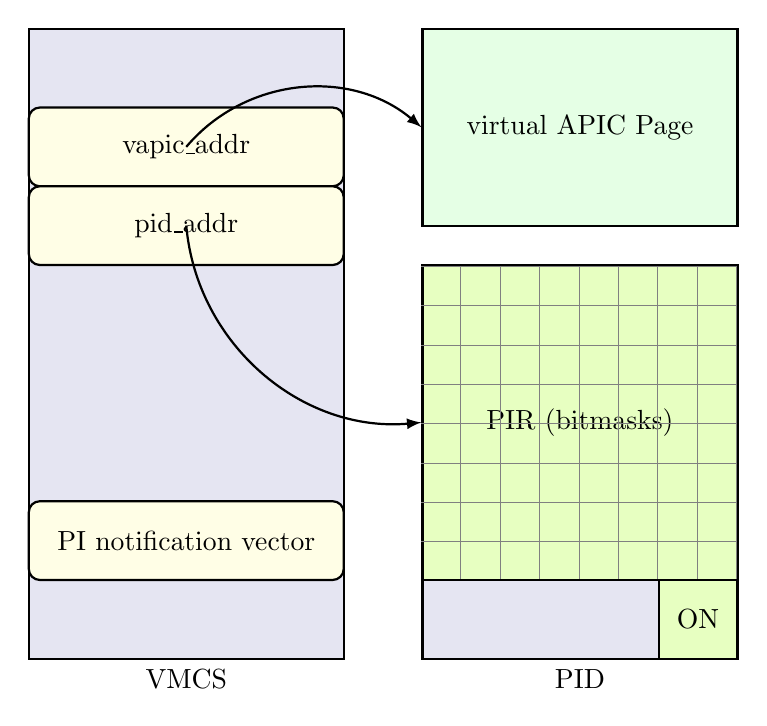
\begin{tikzpicture}


%%\draw[step=0.5cm, gray, very thin] (0,0) grid (9,9);

\node at (0,0) [rectangle, draw=black, thick, fill=NavyBlue!10, minimum height = 8cm, minimum width = 4cm, anchor=south west] (vmcs) {} ;
\node [below, align=center] at (vmcs.south) {VMCS};

\node at (0,6) [rectangle, draw=black, thick, fill=yellow!10, rounded corners, minimum height = 1cm, minimum width = 4cm, anchor=south west] (apicaddr)  {vapic\_addr};
\node at (0,5) [rectangle, draw=black, thick, fill=yellow!10, rounded corners, minimum height = 1cm, minimum width = 4cm, anchor=south west] (pidaddr)  {pid\_addr};

\node at (0,1) [rectangle, draw=black, thick, fill=yellow!10, rounded corners, minimum height = 1cm, minimum width = 4cm, anchor=south west] (pinv)  {PI notification vector};

\node at (5,1) [rectangle, draw=black, thick, fill=GreenYellow!30, minimum height = 4cm, minimum width = 4cm, anchor=south west] (pir) {PIR (bitmasks)};
\begin{scope}[fill opacity=0.9]
	\draw[xstep=0.5cm, ystep=0.5, gray, very thin] (5,1) grid (9,5);
\end{scope}

\node at (5,0) [rectangle, draw=black, thick, fill=NavyBlue!10, minimum height = 1cm, minimum width = 4cm, anchor=south west] (rsrvd) {};
\node at (8,0) [rectangle, draw=black, thick, fill=GreenYellow!30, minimum height = 1cm, minimum width = 1cm, anchor=south west] (on) {ON};
\node [below, align=center] at (rsrvd.south) {PID};

\node at (5,5.5) [rectangle, draw=black, thick, fill=green!10, minimum height = 2.5cm, minimum width = 4cm, anchor=south west] (vapic) {virtual APIC Page};


\begin{scope}[>=latex]
	\draw [thick, ->] (apicaddr.center) to [bend left=45] (vapic.west);
	\draw [thick, ->] (pidaddr.center) to [bend right=45] (pir.west);
\end{scope}


\end{tikzpicture}
\end{center}
\ifreport
\caption{Key data structures for Posted Interrupt processing. Virtual APIC page is used by VT-x to virtualize interrupt controller memory accesses. 
PINV is the interrupt vector number that uses PID data structure for delivery without exit.
PID consists of an ON bit and PIR bitmasks. Host marks PIR bit corresponding to interrupt vector and sets the ON bit
to deliver interrupt directly to the guest.}
\fi
\label{fig-pi-ds}
\end{figure}

PID is a field of VMCS and initialized by the host to inject interrupts owned by guest OS. 
The host also initializes posted interrupt notification vector (PINV) field in VMCS.
PINV is compared in hardware with the physical vector number to decide when an interrupt should be injected directly to the guest.
When an external interrupt whose physical vector is same as PINV arrives and PIR bit for the corresponding vector is set along with outstanding notification (ON) bit the interrupt is delivered to the guest without VM exit transition.
The direct interrupt injection allows reducing virtualization overhead. It allows host to deliver interrupts from devices owned by the guest directly without
intervention. Figure \ref{fig-pi-delivery} shows how virtualization overhead can be reduced by direct interrupt injection mechanism.

\begin{figure}[!htb]
\begin{center}
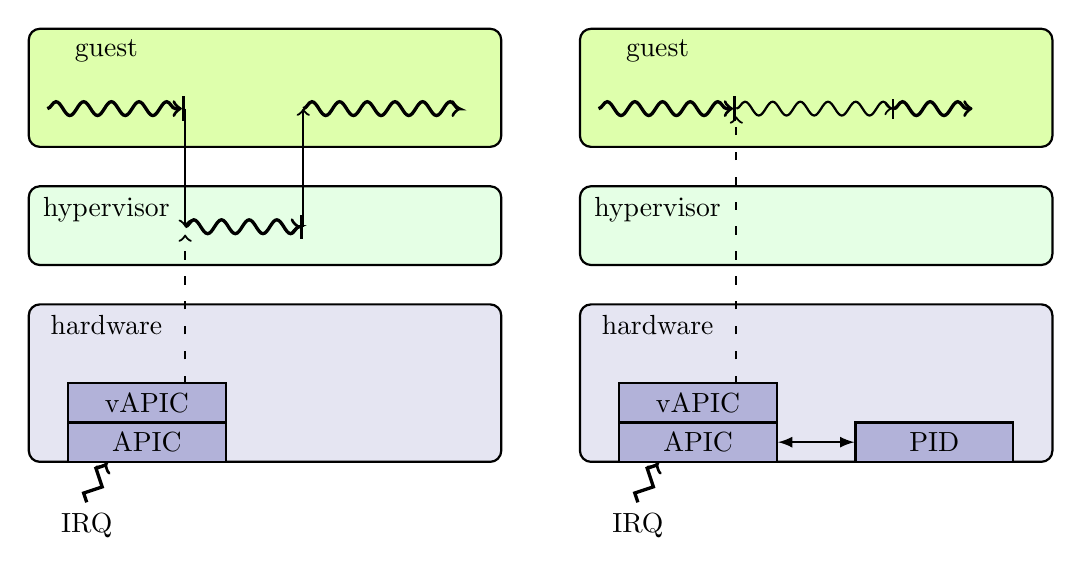
\begin{tikzpicture}


%\draw[step=0.5cm, gray, very thin] (0,0) grid (10,10);

\node at (0,0) [rectangle, draw=black, thick, rounded corners, fill=NavyBlue!10, minimum height = 2cm, minimum width = 6cm, anchor=south west] (hardware1) {} ;
\node at (1,2) [below] {hardware};
\node at (7,0) [rectangle, draw=black, thick, rounded corners, fill=NavyBlue!10, minimum height = 2cm, minimum width = 6cm, anchor=south west] (hardware2) {} ;
\node at (8,2) [below] {hardware};

\node at (0.5,0) [rectangle, draw=black, thick, fill=NavyBlue!30, minimum height = 0.5cm, minimum width = 2cm, anchor=south west] (apic1) {APIC};
\node at (7.5,0) [rectangle, draw=black, thick, fill=NavyBlue!30, minimum height = 0.5cm, minimum width = 2cm, anchor=south west] (apic2) {APIC};

\node at (0.5,0.5) [rectangle, draw=black, thick, fill=NavyBlue!30, minimum height = 0.5cm, minimum width = 2cm, anchor=south west] (vapic1) {vAPIC};
\node at (7.5,0.5) [rectangle, draw=black, thick, fill=NavyBlue!30, minimum height = 0.5cm, minimum width = 2cm, anchor=south west] (vapic2) {vAPIC};

\node at (10.5,0) [rectangle, draw=black, thick, fill=NavyBlue!30, minimum height = 0.5cm, minimum width = 2cm, anchor=south west] (pid2) {PID};

\node at (0,2.5) [rectangle, draw=black, thick, rounded corners, fill=green!10, minimum height = 1cm, minimum width = 6cm, anchor=south west] (phidias1) {} ;
\node at (1,3.5) [below] {hypervisor};
\node at (7,2.5) [rectangle, draw=black, thick, rounded corners, fill=green!10, minimum height = 1cm, minimum width = 6cm, anchor=south west] (phidias2) {} ;
\node at (8,3.5) [below] {hypervisor};

\node at (0,4) [rectangle, draw=black, thick, rounded corners, fill=GreenYellow!40, minimum height = 1.5cm, minimum width = 6cm, anchor=south west] (guest1) {} ;
\node at (1,5.5) [below] {guest};
\node at (7,4) [rectangle, draw=black, thick, rounded corners, fill=GreenYellow!40, minimum height = 1.5cm, minimum width = 6cm, anchor=south west] (guest2) {} ;
\node at (8,5.5) [below] {guest};

\draw[very thick, decorate, decoration=snake, ->|] (0.25, 4.5) -- (2, 4.5);
\draw[thick, ->] (2, 4.5) -- (2, 3);
\draw[very thick, decorate, decoration=snake, ->|] (2.0, 3) -- (3.5, 3);
\draw[thick, ->] (3.5, 3) -- (3.5, 4.5);
\draw[very thick, decorate, decoration=snake, ->] (3.5, 4.5) -- (5.5, 4.5);

\draw[thick, loosely dashed, ->] (2,1) -- (2,2.9);

\draw[very thick, decorate, decoration=snake, ->|] (7.25, 4.5) -- (9, 4.5);
\draw[thick, decorate, decoration=snake, ->|] (9, 4.5) -- (11, 4.5);
\draw[very thick, decorate, decoration=snake, ->] (11, 4.5) -- (12, 4.5);

\draw[thick, loosely dashed, ->] (9,1) -- (9, 4.4);

\draw[very thick, decorate, decoration=zigzag, ->] (0.75, -0.5) -- (1, 0) node at (0.75, -0.5) [below] {IRQ};
\draw[very thick, decorate, decoration=zigzag, ->] (7.75, -0.5) -- (8, 0) node at (7.75, -0.5) [below] {IRQ};


%\begin{scope}[fill opacity=0.9]
%	\draw[xstep=0.5cm, ystep=0.5, gray, very thin] (5,1) grid (9,5);
%\end{scope}

\begin{scope}[>=latex]
	\draw [thick, <->] (apic2.east) to [bend left=0] (pid2);
%	\draw [thick, ->] (pidaddr.center) to [bend right=45] (pir.west);
\end{scope}


\end{tikzpicture}
\end{center}
\ifreport
\caption{Comparison of virtual and direct guest interrupt delivery. 
On left, the guest interrupt is delivered to the hypervisor, and hypervisor injects the interrupt as a virtual interrupt. 
On right, interrupt is directly delivered to the guest using DII mechanism, without hypervisor involvement.}
\fi
\label{fig-pi-delivery}
\end{figure}


\subsubsection{Cache Allocation} \label{sec:cat}
Recent x86 multiprocessor architectures supports up to three levels caches. The first two levels (L1 and L2) are private to the CPU core and L3 (last-level cache) cache is shared between all cores. 
Recently Intel introduced a new feature, called Cache Allocation Technology (CAT), which can be used to partition the last
level cache on the basis of class of service (CLOS). The CLOS is an identifier that can be assigned to a thread or process running on the a CPU core
to ensure quality of service to the application. It can also be used by the hypervisor to assign portion of a cache to a guest.
LLC cache can be partitioned into multiple units by programming a set of registers called capacity bitmasks. Size and number of these registers are
architecture specific, each bit in the mask can correspond to a way in cache. The operating system or hypervisor can use these masks to create 
partitions in the cache where each partition is accessible through CLOS identifier. In order to assign a portion of LLC cache to an application
the operating system or hypervisor assigns CLOS identifier to the application by programming CLOS register on context switch. The underlying hardware ensures 
whenever an access to LLC cache from the application occurs the access goes to only portion of cache assigned to it.

\begin{figure}[!htb]
\begin{center}
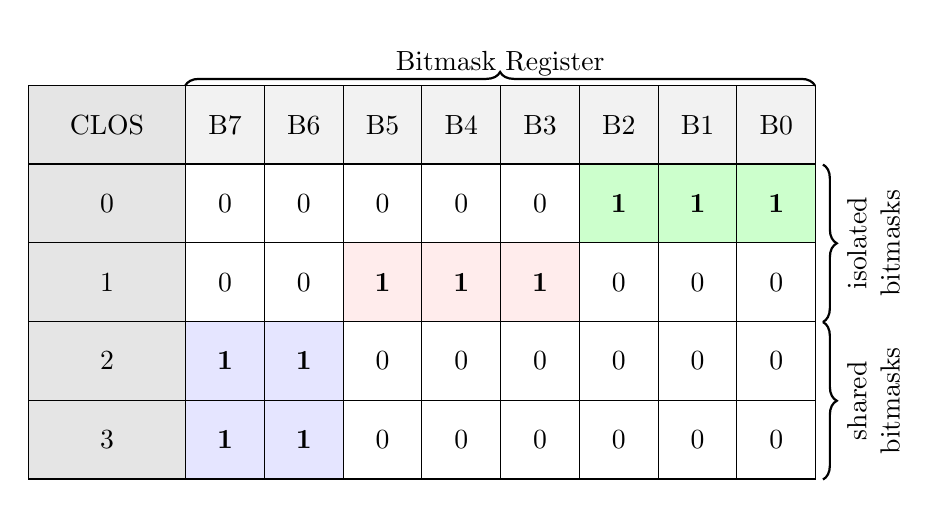
\begin{tikzpicture}

	\foreach \x [evaluate = \bindex using int(8-\x)] in {1,...,8}
		    	\node at (\x,4)[rectangle, draw=black, fill=black!5, minimum height = 1cm, minimum width = 1cm, anchor=south west] (r1\x) 
							{B\bindex};

	\foreach \x in {1,...,8}
				{\ifthenelse{\x>5}
						{\node at (\x,3)[rectangle, draw=black, fill=green!20, minimum height = 1cm, minimum width = 1cm, anchor=south west] (r2\x) {\textbf{1}};}
						{\node at (\x,3)[rectangle, draw=black, fill=white, minimum height = 1cm, minimum width = 1cm, anchor=south west] (r2\x) {0};}

				}
	
		    	%\node at (\x,3)[rectangle, draw=black, fill=white, minimum height = 1cm, minimum width = 1cm, anchor=south west] (r2\x) 
				%			{\ifthenelse{\x>5}{\textbf{1}}{0}};

	\foreach \x in {1,...,8}
				{\ifthenelse{\x>2 \AND \x<6}
						{\node at (\x,2)[rectangle, draw=black, fill=pink!30, minimum height = 1cm, minimum width = 1cm, anchor=south west] (r3\x) {\textbf{1}};}
						{\node at (\x,2)[rectangle, draw=black, fill=white, minimum height = 1cm, minimum width = 1cm, anchor=south west] (r3\x) {0};}
				}
	
		
		    	%% \node at (\x,2)[rectangle, draw=black, fill=white, minimum height = 1cm, minimum width = 1cm, anchor=south west] (r3\x) 
				%%			{\ifthenelse{\x>2 \AND \x<6}{\textbf{1}}{0}};

	\foreach \x in {1,...,8}
				{\ifthenelse{\x<3}
						{\node at (\x,1)[rectangle, draw=black, fill=Blue!10, minimum height = 1cm, minimum width = 1cm, anchor=south west] (r4\x) {\textbf{1}};}
						{\node at (\x,1)[rectangle, draw=black, fill=white, minimum height = 1cm, minimum width = 1cm, anchor=south west] (r4\x) {0};}

				}		    
				%% \node at (\x,1)[rectangle, draw=black, fill=white, minimum height = 1cm, minimum width = 1cm, anchor=south west] (r4\x) 
				%% 			{\ifthenelse{\x<3}{\textbf{1}}{0}};


	\foreach \x in {1,...,8}
				{\ifthenelse{\x<3}
						{\node at (\x,0)[rectangle, draw=black, fill=Blue!10, minimum height = 1cm, minimum width = 1cm, anchor=south west] (r5\x) {\textbf{1}};}
						{\node at (\x,0)[rectangle, draw=black, fill=white, minimum height = 1cm, minimum width = 1cm, anchor=south west] (r5\x) {0};}

				}	
		    	%% \node at (\x,0)[rectangle, draw=black, fill=white, minimum height = 1cm, minimum width = 1cm, anchor=south west] (r5\x) 
				%% 			{\ifthenelse{\x<3}{\textbf{1}}{0}};


	\foreach \y [evaluate = \closindex using int(3-\y)] in {4,...,0}
		    	\node at (-1,\y)[rectangle, draw=black, fill=black!10, minimum height = 1cm, minimum width = 2cm, anchor=south west] (r6\y) 
							{\ifthenelse{\y=4}{CLOS}{\closindex}};

	\draw[thick, decorate, decoration={brace,mirror,amplitude=5pt}] (9.1,2) -- (9.1,4) node [below, align=center, midway, rotate=90, text width=2cm] {\\isolated bitmasks};
	\draw[thick, decorate, decoration={brace,mirror,amplitude=5pt}] (9.1,0) -- (9.1,2) node [below, align=center, midway, rotate=90, text width=2cm] {\\shared bitmasks};

	\draw[thick, decorate, decoration={brace,amplitude=5pt}] (1,5) -- (9,5) node [above, align=center, midway] {\\Bitmask Register};

	%\node (isolatedmasks) at (11, 3) [text width=3cm, align=right]{Isolated Bitmasks};
	%\node (sharedmasks) at (11, 1) [text width=3cm, align=right]{Shared Bitmasks};	

	%\begin{scope}[>=latex]
	%\draw [thick, ->] (r28) to [bend left=45] (isolatedmasks.center);
	%\draw [thick, ->] (r38) to [bend left=45] (isolatedmasks.center);
	%\end{scope}

\end{tikzpicture}
\end{center}
\ifreport
\caption{Example of LLC Partitioning via Bitmasks. Three cache partitions are created by the bitmask registers. 
		First two are isolated ($3/8$ of LLC each) from the rest and the third is shared ($1/4$ of LLC).}
\fi
\label{fig-cat-bitmasks}
\end{figure}

Figure \ref{fig-cat-bitmasks} shows an example where capacity bitmask registers are shown for four applications. The first two masks are 
an example where LLC partitions are isolated. The last two masks give an example where LLC is shared by two applications.

The feature can be used to isolate a real-time guest cache from other guests to ensure any accesses to LLC from GPOS
will not pollute the cache of real-time application. Figure \ref{fig-cat-isolated} gives and example scenario where virtualized software system
uses cache allocation feature to partition LLC of four guests according to bitmasks given in Figure \ref{fig-cat-bitmasks}.
\begin{figure}[!htb]
\begin{center}
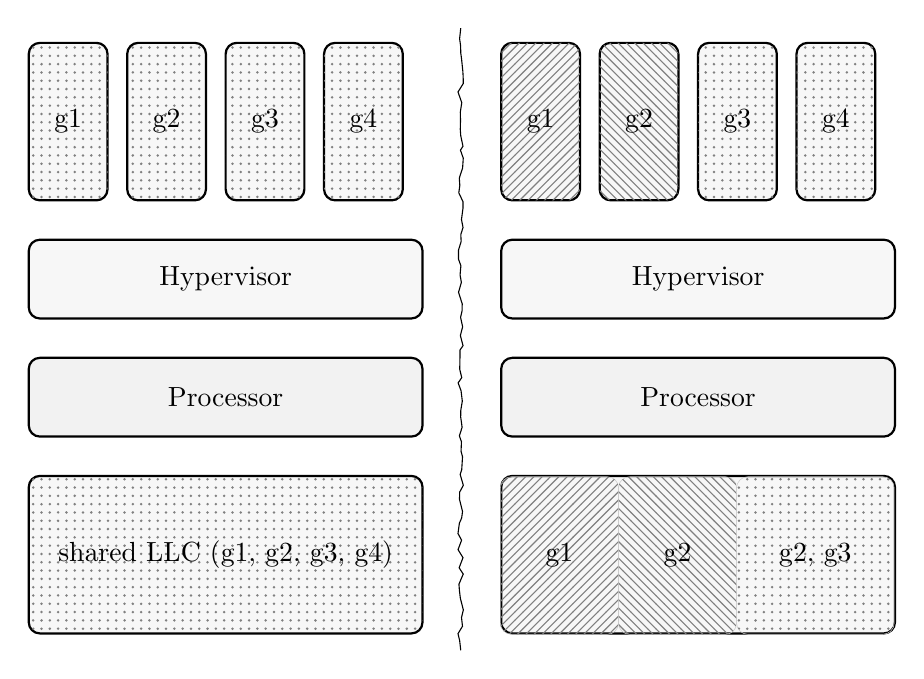
\begin{tikzpicture}


%\draw[step=0.5cm, gray, very thin] (0,0) grid (9,9);


\node at (0,5.5) [rectangle, draw=black, thick, fill=black!3, rounded corners,  postaction={pattern= dots, pattern color=black!50}, minimum height = 2cm, minimum width = 1cm, anchor=south west] (g1) {g1};
\node at (1.25,5.5) [rectangle, draw=black, fill=black!3, thick, rounded corners, postaction={pattern=  dots, pattern color=black!50}, minimum height = 2cm, minimum width = 1cm, anchor=south west] (g2) {g2};
\node at (2.5,5.5) [rectangle, draw=black, fill=black!3, thick, rounded corners, postaction={pattern= dots, pattern color=black!50}, minimum height = 2cm, minimum width = 1cm, anchor=south west] (gN) {g3};
\node at (3.75,5.5) [rectangle, draw=black, fill=black!3, thick, rounded corners, postaction={pattern=  dots, pattern color=black!50}, minimum height = 2cm, minimum width = 1cm, anchor=south west] (gN) {g4};

\node at (6,5.5) [rectangle, draw=black, fill=black!3, thick, rounded corners, postaction={pattern= north east lines, pattern color=black!50}, minimum height = 2cm, minimum width = 1cm, anchor=south west] (g1) {g1};
\node at (7.25,5.5) [rectangle, draw=black, fill=black!3, thick, rounded corners, postaction={pattern= north west lines, pattern color=black!50}, minimum height = 2cm, minimum width = 1cm, anchor=south west] (g2) {g2};
\node at (8.5,5.5) [rectangle, draw=black, fill=black!3, thick, rounded corners, postaction={pattern= dots, pattern color=black!50}, minimum height = 2cm, minimum width = 1cm, anchor=south west] (gN) {g3};
\node at (9.75,5.5) [rectangle, draw=black, fill=black!3, thick, rounded corners, postaction={pattern= dots, pattern color=black!50}, minimum height = 2cm, minimum width = 1cm, anchor=south west] (gN) {g4};

\node at (0,4) [rectangle, draw=black, thick, rounded corners, fill=black!3, minimum height = 1cm, minimum width = 5cm, anchor=south west] (hypervisor1) {Hypervisor} ;
\node at (6,4) [rectangle, draw=black, thick, rounded corners, fill=black!3, minimum height = 1cm, minimum width = 5cm, anchor=south west] (hypervisor2) {Hypervisor} ;

\node at (0,2.5) [rectangle, draw=black, thick, rounded corners, fill=black!5, minimum height = 1cm, minimum width = 5cm, anchor=south west] (cores2) {Processor};
\node at (6,2.5) [rectangle, draw=black, thick, rounded corners, fill=black!5, minimum height = 1cm, minimum width = 5cm, anchor=south west] (cores2) {Processor};

\node at (0,0) [rectangle, draw=black, thick, fill=black!3, rounded corners, postaction={pattern= dots, pattern color=black!50}, minimum height = 2cm, minimum width = 5cm, anchor=south west] (llc1) {shared LLC (g1, g2, g3, g4)};
\node at (6,0) [rectangle, draw=black, thick, rounded corners, fill=black!3, minimum height = 2cm, minimum width = 5cm, anchor=south west] (llc2) {};

\node at (6,0) [rectangle, draw=black!20, very thin, rounded corners, postaction={pattern= north east lines, pattern color=black!50}, minimum height = 2cm, minimum width = 1.5cm, anchor=south west] (g1llc) {g1};
\node at (7.5,0) [rectangle, draw=black!20,  very thin, rounded corners,postaction={pattern= north west lines, pattern color=black!50}, minimum height = 2cm, minimum width = 1.5cm, anchor=south west] (g2llc) {g2};
\node at (9,0) [rectangle, draw=black!20,  very thin, rounded corners,  postaction={pattern= dots, pattern color=black!50}, minimum height = 2cm, minimum width = 2cm, anchor=south west] (g23llc) {g2, g3};

\draw [decorate, decoration={random steps,segment length=3pt,amplitude=1pt}] (5.5,-0.2) -- (5.5,7.7);

\end{tikzpicture}
\end{center}
\ifreport
\caption{Comparison of shared and isolated LLC. One the left is virtual setup when LLC is shared by four guests. On the right is a virtual setup that uses bitmasks from Figure \ref{fig-cat-bitmasks}}
\fi
\label{fig-cat-isolated}
\end{figure}




\section{PHIDIAS Hypervisor}
Provable Hypervisor with Integrated Development Information (PHDIAS) is a multikernel based hypervisor specifically designed to host real-time applications \cite{nordholz2017design}. 
PHIDIAS hypervisor follows design principles that makes it suitable for real-time systems. 
The hypervisor supports multi-core architectures ARM, x86 and MIPS. This section will provide brief description of Phidias hypervisor design, 
implementation on x86 architecture and the mechanisms provided to guest OS.

\subsection{Multikernel Architecture}
Baumann et. al. introduced the idea of multikernel OS architecture for multicore and heterogeneous computer architectures \cite{baumann2009multikernel}. 
The approach removes the requirement of synchronization primitives between software parts executing on different cores by removing the shared memory.
The design approach supports sharing of data between cores using explicit message passing communication primitives.
Phidias uses multikernel design approach where each physical core of the processor runs an instance of Phidias microkernel.
Every instance of the kernel runs in its own address space. The code is shared by all instances but data is private to each instance. 
The hypervisor kernel instance manages virtual machines and only this instance has access to the virtual machine state.
The multikernel model greatly simplifies the design of hypervisor and removes the need of synchronization primitives, 
hence reducing the complexity of the hypervisor.
The multikernel design approach is a matching solution for virtual machines as each VM is running in isolation and 
has nothing to share with other VMs.
In order to support communication between different virtual CPUs of a virtual machine, Phidias supports 
explicit message passing communication mechanism.

\subsection{Principle of Staticity}
The key design idea used to design PHIDIAS is use of principle of staticity.
Jan Nordholz in his PhD thesis \cite{nordholz2017design} has defined the principle of staticity as follows:
\emph {"A hypervisor implementation for an embedded system can
and should be meticulously tailored to its usage scenario. Thus
every element of dynamicity that does not constitute a mandatory 
part of runtime functionality is to be transformed into a
compile-time configuration tool. The retained runtime code is
then purely static, its actions determined by previously generated and externally verifiable configuration data."}

Every real-time embedded application has different requirements and requires a custom tailored solution for the use case. 
Many real-time system go through rigorous testing before they are deployed in the field and require the designers to prove their correctness.
The principle of staticity states that an embedded hypervisor should have no dynamic component, or minimal if there is not other way around.
Phidias uses principle of staticity as a key design rule to ease software provability and reduce run time complexity. 
Removing the dynamic components from the hypervisor also reduces it's footprint which is very attractive for embedded application with limited
memory resources.
The principle of staticity requires that all types of memory requests needed for the virtual machine and devices are known 
before integration of the software systems.

The Phidias hypervisor uses an XML based system configuration tool to create virtual machine configuration and generate
core of the hypervisor. Phidias supports static partitioning of hardware resources. 
Each guest operating system is assigned a subset of processing elements, memory space and IO devices.
Figure \ref{fig-static-part} shows an example configuration scenario where CPU cores and memory divided between the guests.
The principle of staticity is used by Phidias to completely remove memory allocation system.
The memory allocater is removed by creating static page-tables from system descriptions, for both the hypervisor and the virtual machines.
The device emulation core also uses principle of staticity to create and add custom tailored emulation core,
hence reducing the run time complexity.

\begin{figure}[!htb]
\begin{center}
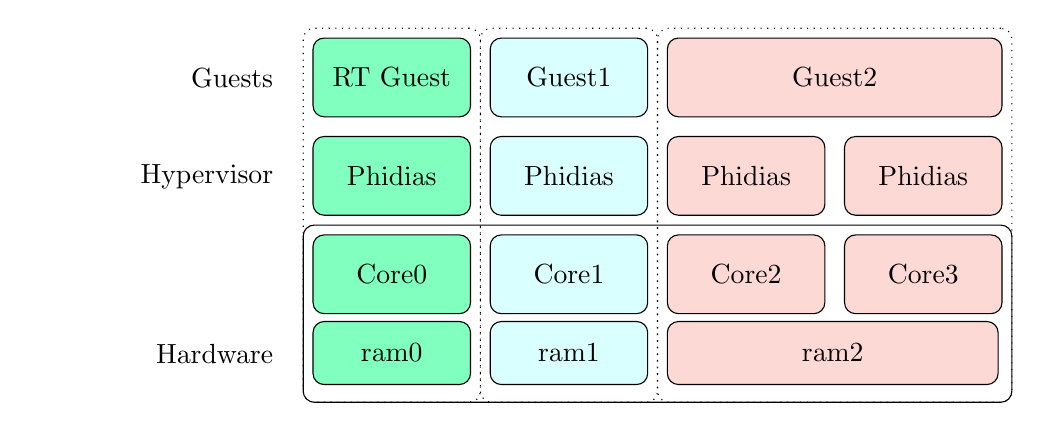
\begin{tikzpicture}

\node at (0,0)[rectangle, draw=black, fill=SpringGreen!50, rounded corners, minimum height = 1cm, minimum width = 2cm, anchor=south west] (core0) {Core0};
\node at (2.25,0)[rectangle, draw=black, fill=Cyan!15, rounded corners, minimum height = 1cm, minimum width = 2cm, anchor=south west] (core1) {Core1};
\node at (4.50,0)[rectangle, draw=black, fill=Salmon!30, rounded corners, minimum height = 1cm, minimum width = 2cm, anchor=south west] (core2) {Core2};
\node at (6.75,0)[rectangle, draw=black, fill=Salmon!30, rounded corners, minimum height = 1cm, minimum width = 2cm, anchor=south west] (core3) {Core3};

\node at (0,-0.9) [rectangle, draw=black, fill=SpringGreen!50, rounded corners, minimum height = 0.8cm, minimum width = 2cm, anchor=south west] (ram0) {ram0};
\node at (2.25,-0.9) [rectangle, draw=black, fill=Cyan!15, rounded corners, minimum height = 0.8cm, minimum width = 2cm, anchor=south west] (ram1) {ram1};
\node at (4.50,-0.9) [rectangle, draw=black, fill=Salmon!30, rounded corners, minimum height = 0.8cm, minimum width = 4.2cm, anchor=south west] (ram2) {ram2};

\begin{scope}[fill opacity=0.0]
\node at (-0.125,-0.125-1)[rectangle, draw=black, fill=white, rounded corners, minimum height = 2.25cm, minimum width = 9.00cm, anchor=south west] (hardware) {};

\node at (-0.125,-1.125)[rectangle, draw=black, fill=black!5, dotted, rounded corners, minimum height = 4.75cm, minimum width = 2.25cm, anchor=south west] (rtg) {};
\node at (2.125,-1.125)[rectangle, draw=black, fill=black!2, dotted, rounded corners, minimum height = 4.75cm, minimum width = 2.25cm, anchor=south west] (g1) {};
\node at (4.375,-1.125)[rectangle, draw=black, fill=black!6, dotted, rounded corners, minimum height = 4.75cm, minimum width = 4.50cm, anchor=south west] (g2) {};

\end{scope}

\node at (0.0,1.25)[rectangle, draw=black, fill=SpringGreen!50, rounded corners, minimum height = 1cm, minimum width = 2cm, anchor=south west] {Phidias};
\node at (2.25,1.25)[rectangle, draw=black, fill=Cyan!15, rounded corners, minimum height = 1cm, minimum width = 2cm, anchor=south west] {Phidias};
\node at (4.50,1.25)[rectangle, draw=black, fill=Salmon!30, rounded corners, minimum height = 1cm, minimum width = 2cm, anchor=south west] {Phidias};
\node at (6.75,1.25)[rectangle, draw=black, fill=Salmon!30, rounded corners, minimum height = 1cm, minimum width = 2cm, anchor=south west] {Phidias};

\node at (0.0,2.5)[rectangle, draw=black, fill=SpringGreen!50, rounded corners, minimum height = 1cm, minimum width = 2cm, anchor=south west] {RT Guest};
\node at (2.25,2.5)[rectangle, draw=black, fill=Cyan!15, rounded corners, minimum height = 1cm, minimum width = 2cm, anchor=south west] {Guest1};
\node at (4.50,2.5)[rectangle, draw=black, fill=Salmon!30, rounded corners, minimum height = 1cm, minimum width = 4.25cm, anchor=south west] {Guest2};

\node (hardware) at (-2.0, -0.5) [text width=3cm, align=right]{Hardware};
\node (phidias) at (-2.0, 1.75) [text width=3cm, align=right]{Hypervisor};
\node (guests) at (-2.0, 3.0) [text width=3cm, align=right]{Guests};

\end{tikzpicture}
\end{center}
\ifreport
\caption{Example partitioning of a multicore x86 platform using Phidias. The guests are allocated separate CPU cores and RAM memory. 
Since Phidias follows multikernel design approach, an instance of Phidias runs on each core.}
\fi
\label{fig-static-part}
\end{figure}


\subsection{Non-Preemptible Kernel}
Phidias hypervisor kernel is non-preemptible and interrupts are always disabled when hypervisor executes. 
Preemptibility means a higher priority task can preempt currently running task until it finishes and lower priority task is then resumed.
An RTOS is always designed to be preemptible, even the GPOS also provide voluntary preemption.

Preemptible kernels sound great, however it is achieved at the cost of higher software complexity.  
It introduces new execution paths in the kernel and makes is difficult to prove correctness of the software system.
Since the software can be preempted at any point by a high priority task the kernel has to support context switching and
synchronization primitives to ensure correct software behavior.

Non-preemptibility can be tolerated if all execution path in the hypervisor are kept very short, which is true for Phidias.
To keep low software complexity and footprint preemption is not supported by Phidias.
Phidias hypervisor kernel paths are very short that simplifies the software design and makes it easier to prove correctness.

\subsection{Inter-VM Communication}
Phidias supports asynchronous communication between virtual machines.
Virtual machines can transfer data between each other through communication channels that
are configured statically before deploying software system.
A communication channel consists of shared buffer and a virtual interrupt for signaling.
The VM stores data in shared buffer and generates an interrupt to inform receiver.
Phidias injects a virtual interrupt to the receiving VM to inform availability of data.
Phidias does not support creation of communication channels at run time.

\subsection{Small TCB}
Since Phidias uses principle of staticity that eliminates dynamic parts and non-preemptive
kernel to reduce hypervisor complexity, the resulting hypervisor has very small code size.
The small code size of the hypervisor results in small trusted computing base (TCB).
Small TCB increases the confidence in software system's security.
The overhead of formal verification and mathematical proof reduces significantly.


\subsection{Guest Device Handling} 
Phidias hypervisor supports three mechanisms to interface guest devices, a brief introduction to each mechanism is provide in this section.
Figure \ref{fig-device-handling} shows difference between the three device handling mechanisms supported.
\begin{figure}[!htb]
\begin{center}
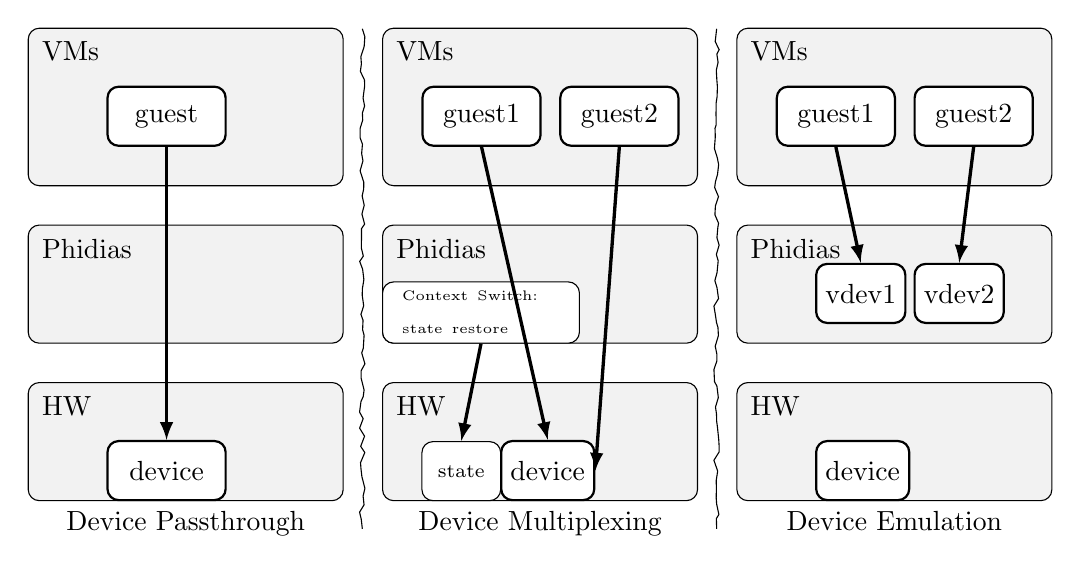
\begin{tikzpicture}

\node at (0,4)[rectangle, draw=black, fill=black!5, rounded corners, minimum height = 2cm, minimum width = 4cm, anchor=south west] (vms1) {};
\node[below right, inner sep=5pt] at (vms1.north west) {VMs};
\node at (4.5,4)[rectangle, draw=black, fill=black!5, rounded corners, minimum height = 2cm, minimum width = 4cm, anchor=south west] (vms2) {};
\node[below right, inner sep=5pt] at (vms2.north west) {VMs};
\node at (9,4)[rectangle, draw=black, fill=black!5, rounded corners, minimum height = 2cm, minimum width = 4cm, anchor=south west] (vms3) {};
\node[below right, inner sep=5pt] at (vms3.north west) {VMs};

\node at (0,2)[rectangle, draw=black, fill=black!5, rounded corners, minimum height = 1.5cm, minimum width = 4cm, anchor=south west] (phidias1) {};
\node[below right, inner sep=5pt] at (phidias1.north west) {Phidias};
\node at (4.5,2)[rectangle, draw=black, fill=black!5,  rounded corners, minimum height = 1.5cm, minimum width = 4cm, anchor=south west] (phidias2) {};
\node[below right, inner sep=5pt] at (phidias2.north west) {Phidias};
\node at (9,2)[rectangle, draw=black, fill=black!5, rounded corners, minimum height = 1.5cm, minimum width = 4cm, anchor=south west] (phidias3) {};
\node[below right, inner sep=5pt] at (phidias3.north west) {Phidias};

\node at (0,0)[rectangle, draw=black, fill=black!5, rounded corners, minimum height = 1.5cm, minimum width = 4cm, label=south:Device Passthrough,anchor=south west] (hw1) {};
\node[below right, inner sep=5pt] at (hw1.north west) {HW};
\node at (4.5,0)[rectangle, draw=black, fill=black!5, rounded corners, minimum height = 1.5cm, minimum width = 4cm, label=south:Device Multiplexing, anchor=south west] (hw2) {};
\node[below right, inner sep=5pt] at (hw2.north west) {HW};
\node at (9,0)[rectangle, draw=black, fill=black!5, rounded corners, minimum height = 1.5cm, minimum width = 4cm, label=south:Device Emulation, anchor=south west] (hw3) {};
\node[below right, inner sep=5pt] at (hw3.north west) {HW};

\node at (1,4.5)[thick, rectangle, draw=black, fill=white, rounded corners, minimum height = 0.75cm, minimum width = 1.5cm, anchor=south west] (g11) {guest};
\node at (1,0)[thick, rectangle, draw=black, fill=white, rounded corners, minimum height = 0.75cm, minimum width = 1.5cm, anchor=south west] (dev1) {device};
\begin{scope}[>=latex]
	\draw [very thick, ->] (g11.south) to [bend right=0] (dev1.north);
\end{scope}

\node at (5,4.5)[thick, rectangle, draw=black, fill=white, rounded corners, minimum height = 0.75cm, minimum width = 1.5cm, anchor=south west] (g21) {guest1};
\node at (6.75,4.5)[thick, rectangle, draw=black, fill=white, rounded corners, minimum height = 0.75cm, minimum width = 1.5cm, anchor=south west] (g22) {guest2};
\node at (4.5,2.0)[rectangle, draw=black, fill=white,  rounded corners, minimum height = 0.75cm, minimum width = 2.5cm, text width=2cm, anchor=south west] (hyp2st) 
					{\tiny{Context Switch: state restore}};
\node at (5,0)[rectangle, draw=black, fill=white, rounded corners, minimum height = 0.75cm, minimum width = 1cm, anchor=south west] (dev2st) {\scriptsize{state}};
\node at (6,0)[thick, rectangle, draw=black, fill=white, rounded corners, minimum height = 0.75cm, minimum width = 1cm, anchor=south west] (dev2) {device};
\begin{scope}[>=latex]
	\draw [very thick, ->] (g21.south) to [bend right=0] (dev2.north);
	\draw [very thick, ->] (g22.south) to [bend right=0] (dev2.east);
	\draw [very thick, ->] (hyp2st.south) to [bend right=0] (dev2st.north);
\end{scope}


\node at (9.5,4.5)[thick, rectangle, draw=black, fill=white, rounded corners, minimum height = 0.75cm, minimum width = 1.5cm, anchor=south west] (g31) {guest1};
\node at (11.25,4.5)[thick, rectangle, draw=black, fill=white, rounded corners, minimum height = 0.75cm, minimum width = 1.5cm, anchor=south west] (g32) {guest2};
\node at (10,2.25)[thick, rectangle, draw=black, fill=white, rounded corners, minimum height = 0.75cm, minimum width = 1cm, anchor=south west] (vdev1) {vdev1};
\node at (11.25,2.25)[thick, rectangle, draw=black, fill=white, rounded corners, minimum height = 0.75cm, minimum width = 1cm, anchor=south west] (vdev2) {vdev2};
\node at (10,0)[thick, rectangle, draw=black, fill=white, rounded corners, minimum height = 0.75cm, minimum width = 1cm, anchor=south west] (dev3) {device};
\begin{scope}[>=latex]
	\draw [very thick, ->] (g31.south) to [bend right=0] (vdev1.north);
	\draw [very thick, ->] (g32.south) to [bend right=0] (vdev2.north);	
\end{scope}

\draw [decorate, decoration={random steps, segment length=3pt,amplitude=1pt}] (4.25,-0.35) -- (4.25,6);
\draw [decorate, decoration={random steps, segment length=3pt,amplitude=1pt}] (8.75,-0.35) -- (8.75,6);

\end{tikzpicture}
\end{center}
\ifreport
\caption{Device handling mechanisms supported by Phidias}
\fi
\label{fig-device-handling}
\end{figure}


\subsubsection{Device Passthrough}
The device passthrough mechanism allows a guest to take complete ownership of a device. 
The virtual machine interacts with the device without any intervention from the hypervisor.
Memory mapped devices are passed to the guest by giving complete ownership of the device memory region. 
In this case, the Phidias configuration tool enables addition of an entry in the static nested page-tables of the owner guest 
for exclusive read write access of the device memory.
On contrary some devices are IO mapped, in which case exclusive access to that IO region is given to the owner guest.
The device passthrough mechanism results in highest performance however it is suitable only when a guest exclusively owns the device.

\subsubsection{Device Multiplexing}
If same device is accessed from multiple guests then Phidias hypervisor supports multiplexing of the device between guests. 
Device multiplexing is achieved by restoring the device state for a guest whenever context switch takes place. 
The current state of the device is saved until the context switch happens again. 
Saving and restoring device state on context switch add small overhead however once completed the device can be accessed exclusively by the guest OS.
This mechanism can only be supported for devices that are virtualization aware and expose their complete state.
Another situation when the mechanism can be useful is if the guests use same state for the device, in such scenario even the overhead of 
state restore can be saved.

\subsubsection{Device Emulation}
Device emulation is the only choice of device handling if the device does not exist on the hardware or it is not virtualization aware.
The behavior of the device is completely emulated by the hypervisor in software and guest OS is oblivious to the fact that device does not exist on the hardware.
All requests to the target device are trapped and emulated by the host software. This mechanism has the largest overhead due to emulation of device in software.

\subsubsection{Static Configuration Tool}
Phidias hypervisor kernel itself is created through a static configuration tool. 
As stated earlier, the hypervisor uses principle of staticity as the main design goal to ease provability and lower the software complexity.
Principle of staticity requires all configuration of the hypervisor kernel and virtual machines to be enlisted prior to creation of hypervisor executable. 
The static configuration tool takes the configuration as input and creates all necessary data structures to configure the hypervisor microkernel. 
The configuration tool also generates page-tables data structures for hypervisor and nested page-tables for each virtual machine. 
All page-table structures are transformed to binary and packaged into the final executable of the software system.


\subsection{Implementation on x86}
This section will give a brief overview of Phidias implementation on Intel x86 platform.

Phidias utilizes Intel virtualization extensions to implement faithful virtualization. 
It uses extended page-table (Intel EPT) feature for MMU virtualization. 
And supports per core local APIC virtualization through software
emulation or by using hardware virtualization technique for APIC virtualization (APIC-v).

The hypervisor executes in VM root operation mode and launches virtual machines that run in VM non-root operation mode.
Hypervisor configures virtual machine control structure (VMCS) to cause vmexit transition if guest tries to execute an IO operation, on arrival of an external interrupt, and or guest tries to execute of a privileged instruction.  
The hypervisor takes control when such a situation occurs, emulates desired behavior and returns control back to the virtual machine through vmentry transition. 
Phidias only handles exceptions for nested page-tables, the guest has complete control over exceptions that may occur on guest page-tables.
The nested page-table exceptions are configured as traps and used to emulate device accesses. 

Recent Intel virtualization extensions support optimizing hypervisor operation for guest access to machine specific registers and IO ports through bitmaps.
Phidias hypervisor supports all these mechanisms to lower virtualization overhead. 

In order to perform useful operations, a Linux guest requires a least four devices: a timer as clocksource, a timer for event generation, an interrupt controller, and a serial interface for input/output. The event generation and clock source timers can use the same timer infrastructure, however on x86 these two can be different. Phidias supports these minimal set of devices per guest, details of implementation follows:

\subsubsection{Interrupt Controller}
An interrupt controller is a programmable logic circuit inside the microprocessor chip that allows processor core to configure and control interrupts.
CPU associates an individual interrupt source with an interrupt vector by writing the vector number into the corresponding interrupt controller register.
This interrupt vector number is given to the processor by interrupt controller when an interrupt arrives from the particular source, which allows CPU to
recognize source of interrupt. The interrupt controller also allows CPU to disable an individual interrupt.

The x86 multiprocessor architecture supports two types of interrupt controllers.
An interrupt controller per physical CPU core, known as local advanced programmable interrupt controller (LAPIC).
And at least one interrupt controller to configure interrupts from external IO devices, known as IOAPIC.
LAPIC is used to configure interrupts local to CPU core and to send and receive inter-processor interrupts (IPIs).
IOAPIC is used to receive interrupts from devices external to the multiprocessor chip.
Some external devices also send interrupts to the microprocessor chip on system bus, these interrupt are called Message Signaled Interrupts (MSIs).
Interrupts delivered by PCIe cards is an example of this type of interrupt.
LAPIC is responsible to decode these interrupts and forward them to the core.

Phidias hypervisor supports emulation of local APIC in software. 
In this case a software state of APIC is maintained for the guest while the actual hardware is in full control of the hypervisor.
Phidias also also supports hardware-based APIC virtualization (APIC-v).
The APIC virtualization feature allows reducing software emulation time by emulating read/write access in hardware.
The processor keeps track of virtual APIC core and allows virtual interrupt delivery without hypervisor intervention.

The IOAPIC interrupt controller is emulated by Phidias in software by keeping a software state of IOAPIC. 
External interrupts are received by Phidias and virtual IOAPIC states of each guest is consulted to inject and a virtual interrupt to that guest.
The hypervisor supports two types of virtual interrupt injection mechanisms.
When an interrupt source is shared between guests, the hypervisor injects virtual interrupts to the guests.
If a guest is the only owner of the interrupt, it allows interrupt passthrough or direct interrupt injection using APIC virtualization.
When interrupt passthrough is used then hypervisor takes the interrupt and passes it to the hypervisor without further processing, keeping the kernel execution path short. 
When direct interrupt injection is used, the hypervisor uses APIC virtualization to inject virtual interrupt to the guest without hypervisor intervention.

\subsubsection{Timer as Event Generator}
Linux guest on x86 platform uses per core local APIC timer (LAPIC timer) to generate events. 
The local APIC core supports various modes of operation for event generation: periodic, one-shot or TSC-deadline mode. 
Phidias uses LAPIC timer core to emulate guest timer events.
It has a generic timer infrastructure to generate timer events and supports all modes of operations desired by the guest. 
The timer infrastructure keeps a queue of time events sorted by the event deadline.
Event with earliest deadline is programmed into the LAPIC timer, when timer expires the event is forwarded to the requesting guest.
The same timer event generation infrastructure is used by the hypervisor scheduler to trigger scheduling events.

\subsubsection{Timer as Clock Source}
In addition to event generation Linux guest uses a monotonically increasing timer source as its clocksource. 
Guest uses this timer to keep track of time. 
On x86 platform Linux guest uses time-stamp counter (TSC) as the clock source. 
TSC increments monotonically at the processor clock speed and keeps the count value in 64-bit register.
Phidias hypervisor support TSC counter as a pass-through device.
The current value of the TSC counter is always available to the guest without hypervisor intervention.
In order to keep the illusion that guest is running directly on the hardware, Phidias supports TSC-offsetting feature.
TSC-offsetting feature allows host to offset the counter value to compensate for time quantum for which host executes on the hardware.
%This feature allows adding an offset value to the actual TSC timer value. 
PHIDIAS configures the offset value to the time that lapses between vmexit and vmentry.

\subsubsection{Serial Interface}
A serial interface is very useful for a guest to interact with user and dump debugging information.
Phidias hypervisor support one serial interface per guest by emulating UART 16650 interface of x86 architecture.
The hypervisor uses the same interface to dump its own debug information. 
The emulation works in conjunction to a small tool on the host side that supports multiplexing of the interface between the guests and the hypervisor itself.
The multiplexer tool opens up one console per guest and one for the hypervisor. When a request to dump information from a guest arrives the hypervisor
sends this debug information to the serial interface. A special code sequence is sent to the console every time the interface is switched between the guests.
The code sequence is used by the host tool to differentiate where to dump incoming information. 
Similarly when user wants to interact with a virtual machine, a special code sequence is sent to hypervisor.
This time the code sequence helps hypervisor to decide to which guest the input shall be routed. 

\chapter{Virtualization Overhead\label{chap3}}

This chapter presents analysis of virtualization overhead for Phidias hypervisor and records 
results of experiments conducted on x86 platform. 
In order to evaluate virtualization overhead of x86 processor a hypothetical mixed criticality system is used
that includes an RTOS and GPOS running concurrently in separate virtual machines.
The key parameter used to measure the overhead is real-time event handling latency, also known as 
interrupt response time (IRT).
The interrupt latency is the time that elapses between arrival of an external interrupt request (IRQ) and execution of event handler starts.
Figure \ref{fig-latency-keymetric} depicts the difference in interrupt latency experienced by and external interrupt request in native and
virtualized environment.
In a virtual setup the latency is expected to increase due to hypervisor intervention when external interrupt are routed to guest through hypervisor.
The hypervisor injects external interrupts to owner guest by servicing interrupt first. Execution of hypervisor before interrupt is passed to 
the owner guest increases the interrupt latency.
It is important to measure virtualization overhead to determine if deadlines of the real-time tasks of guest RTOS can still be respected.

\begin{figure}[!htb]
\begin{center}
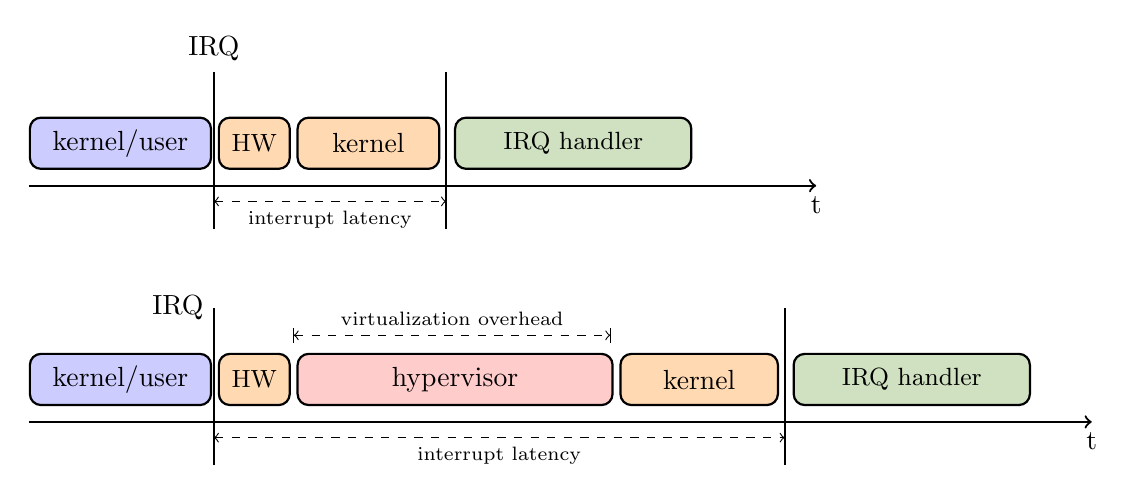
\begin{tikzpicture}

\newcommand\yh{0.65cm}

%\draw[step=1cm, gray, very thin, dotted] (0,0) grid (15,6);

\node at (0,4) [rectangle, draw=black, thick, fill=Blue!20, rounded corners, minimum height = \yh, minimum width = 2.3cm, anchor=south west] (kubefore) 
				{kernel/user};
\node at (2.4,4) [rectangle, draw=black, thick, fill=orange!30, rounded corners, minimum height = \yh, minimum width = 0.9cm, anchor=south west] (hardware) 
				{\small{HW}};
\node at (3.4,4) [rectangle, draw=black, thick, fill=orange!30, rounded corners, minimum height = \yh, minimum width = 1.8cm, anchor=south west] (kservice) {kernel};
\node at (5.4,4) [rectangle, draw=black, thick, fill=OliveGreen!20, rounded corners, minimum height = \yh, minimum width = 3cm, anchor=south west] (kuafter) {\small{IRQ} handler};
\draw[black, thick] (2.35,3.25) -- (2.35,5.25) node [above] {IRQ};
\draw[black, thick] (5.3,3.25) -- (5.3,5.25) node [above] {};
\draw[black, dashed, <->] (2.35,3.6) -- (5.3,3.6) node [below, align=center, midway] {\scriptsize{interrupt latency}};

\draw[black, thick, ->] (0,3.8) -- (10,3.8) node at (10,3.8) [below] {t};

\node at (0,1) [rectangle, draw=black, thick, fill=Blue!20, rounded corners, minimum height = \yh, minimum width = 2.3cm, anchor=south west] (kubefore) {kernel/user};
\node at (2.4,1) [rectangle, draw=black, thick, fill=orange!30, rounded corners, minimum height = \yh, minimum width = 0.9cm, anchor=south west] (hardware) 
				{\small{HW}};

\node at (3.4,1) [rectangle, draw=black, thick, fill=red!20, rounded corners, minimum height = \yh, minimum width = 4cm, anchor=south west] (hyper) {hypervisor};

\node at (7.5,1) [rectangle, draw=black, thick, fill=orange!30, rounded corners, minimum height = \yh, minimum width = 2cm, anchor=south west] (kservice) {kernel};
\node at (9.7,1) [rectangle, draw=black, thick, fill=OliveGreen!20, rounded corners, minimum height = \yh, minimum width = 3cm, anchor=south west] (kuafter) {\small{IRQ} handler};

\draw[black, thick] (2.35,0.25) -- (2.35, 2.25)  node [left] {IRQ};
%\draw[black, thick] (7.4, 0.65) -- (7.4, 2.25) node [above] {};
\draw[black, thick] (9.6,0.25) -- (9.6, 2.25) node [above] {};

\draw[black, dashed, |<->|] (3.35,1.9) -- (7.4,1.9) node [above, align=center, midway] {\scriptsize{virtualization overhead}};
\draw[black, dashed, <->] (2.35,0.6) -- (9.6,0.6) node [below, align=center, midway] {\scriptsize{interrupt latency}};


\draw[black, thick, ->] (0,0.8) -- (13.5,0.8) node at (13.5,0.8) [below] {t};

\end{tikzpicture}
\end{center}
\ifreport
\caption{Interrupt Latency in native and virtualized environment}
\fi
\label{fig-latency-keymetric}
\end{figure}


Hypervisor overhead consists for context switch times, execution of hypervisor code to identify and inject virtual interrupt to the real-time guest (rt-guest) and
resource contention. The resource contention overhead arises due to shared resources between guests and hypervisor.
While this chapter focuses on analyzing and measuring components of virtualization overhead, the next chapter covers techniques to lower overhead components.

\section{Experimental Setup} 
All experiments are conducted on Intel Xeon E5-2603v4 processor \cite{intel-ark-xeon} mounted on ASUS X99E WS motherboard \cite{asus-x99e}. 
The processor runs at $1.7GHz$ clock speed and had access to $4GB$ RAM memory.
This processor contains $6$ physical CPU cores where each core has private L1 and L2 caches, the cache capacities are $64KB$ and $512KB$ respectively.
The last-level cache (L3) is shared shared between cores and has 15MB capacity. 
The processor supports Intel VT-x technology. The virtualization extensions on Xeon processor includes virtualization of LAPIC and MMU.

The evaluated virtualization solution contains hypervisor and two guests: an RTOS and a GPOS.
RTOS guest has been created by applying latest PREEMPT\_RT patchset (v4.11.12-rt15) to Linux kernel (v4.11.12).
The details of PREEMPT\_RT patch are covered in section \ref{sec:rtos-ext-gpos}.
The GPOS guest is Linux kernel (v4.11.8).
A small patchset was applied to both real-time and general purpose Linux operating systems, given in appendix \ref{app:a}.
Linux kernel uses PIT (Programmable Interval Timer) to calculate processor clock frequency during bootup process.
Phidias hypervisor does not support virtualization of PIT device at the moment, the patch is used to fix processor clock frequencies to known values.


An external device on PCIe (Peripheral Component Interconnect Express) bus manufactured by VersaLogic is used to generate external events \cite{versalogic}.
The device is equipped with EXAR XR17v354 SoC \cite{xr17v354} and supports up to 12 general purpose input/outputs (GPIOs). 
The VersaLogic GPIO device has the capability to send Message Signaled Interrupts (MSIs) to the processor when an external event is detected.
Each GPIO can be programmed to cause an external interrupt when a rising pulse is detected on the inputs.
The RTOS guest was given full access to the device by granting read/write accesses to the device memory.
Furthermore real-time guest was given full access to HPET (High Precision Event Timer) device. 
The HPET device is needed by cyclictest\cite{cyclictest}, a widely used tool to evaluate real-time performance of PREEMPT\_RT Linux kernel.
The cyclictest has been used for two purposes. First, it was used to validate latency results produced for gpio device interrupts.
Secondly, it was used as load to exercise POSIX thread operations as explained in next section.
Table \ref{experiment-setup} summarizes setup used to conduct experiments.


\begin{table}[!htbp]
\centering
%\begin{longtable}{|p{.20\textwidth} | p{.70\textwidth}|}
\begin{longtable}{|p{2cm}|p{2cm}|p{6cm}|p{2cm}|}  
\hline
\textbf{Resource} & \textbf{CPUs} & \textbf{Devices} & \textbf{Physical Memory} \\ \hline 
RTOS & & & \\ 
(rt-guest) & one vCPU & vLAPIC, vIOAPIC, vLAPIC-Timer, vUART, PCIe GPIO, HPET & 256MB \\ \hline
GPOS & & & \\ 
(gp-guest) & one vCPU & vLAPIC, vIOAPIC, vLAPIC-Timer, vUART & 256MB \\ \hline
PHIDIAS & & & \\ 
Hypervisor & two cores & LAPIC, IOAPIC, LAPIC Timer, UART & -- \\ \hline
Hardware & \multicolumn{3}{|c|}{Xeon  E5-2603v4 Processor} \\ \hline
\caption{Experiment Setup}
\label{experiment-setup}
\end{longtable}
\end{table}

\section{Measurement Setup} \label{sec:measurement-setup}
The interrupt latency measurement setup consists of an external FPGA board \cite{terasic-de0nano} and external PC for latency measurement.
Two GPIOs of FPGA are connected to PCIe GPIO device. First one to cause an interrupt and send low-to-high pulse and second to listen for
response time of GPIO interrupt handler. External PC sends commands to FPGA on UART to generate an interrupt.
The measurement setup generates an interrupt for rt-guest and expects rt-guest to respond by asserting an output GPIO.

A small patch for EXAR XR17v354 SoC was added to rt-guest to configure GPIOs for desired behavior.
And a separate kernel module was designed and loaded on rt-guest to register interrupt handler for the PCIe GPIO device.
Source code for added gpio device functionality and interrupt handler module is given in appendix \ref{app:a}.
The very first instruction executed by gpio interrupt handler is assertion of an output pin, to mark time instance when interrupt handler starts execution.
The pin assertion marks the response time of gpio interrupt handler.
It allows external setup to measure latency by calculating time difference between observed response time and interrupt generation.
The FPGA hardware is programmed to perform a routine as follows:
\begin {itemize}
	\item {wait to receive command from external PC on UART interface}
	\item {generate interrupt for rt-guest by asserting input GPIO of PCIe device}
	\item {count FPGA clock cycles while waiting rt-guest interrupt handler to send response on output GPIO}
	\item {send counted clock cycles to external PC on UART interface}
\end {itemize}

Figure \ref{fig-measure-steup} describes measurement setup and demonstrates how GPIOs are used to measure latency.
The external PC calculates interrupt latency by scaling the count value by known FPGA clock frequency (50MHz). 
A small script on external PC can be used to repeat measurement routine multiple time to find worst-case interrupt latency.


\begin{figure}[!htb]
\begin{center}
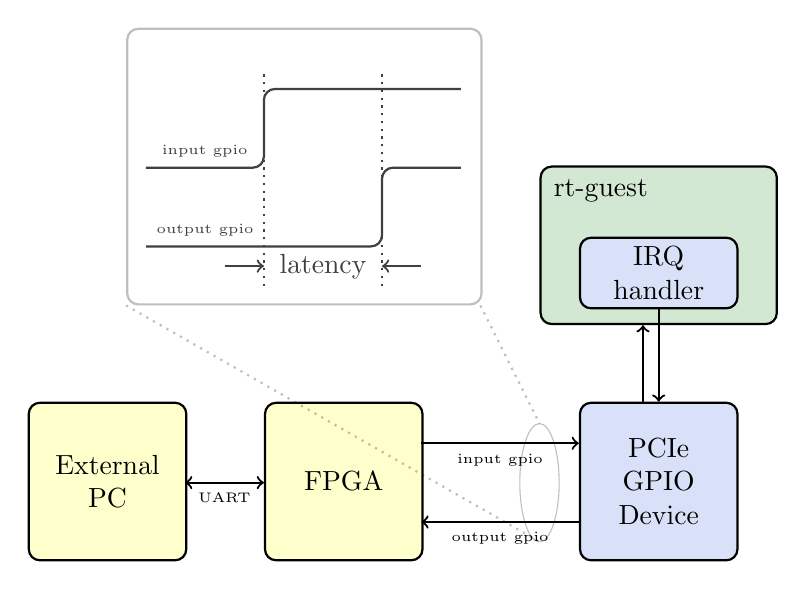
\begin{tikzpicture}

%\draw[step=1cm, gray, very thin, dotted] (0,0) grid (10,8);

\node at (0,0) [rectangle, draw=black, thick, fill=Yellow!20, rounded corners, minimum height = 2cm, minimum width = 2.0cm, align=center, text width=1.7cm, anchor=south west] (pc) 
		{External\\ PC};

\node at (3,0) [rectangle, draw=black, thick, fill=Yellow!20, rounded corners, minimum height = 2cm, minimum width = 2cm, anchor=south west] (fpga) 
		{FPGA};

\node at (7,0) [rectangle, draw=black, thick, fill=RoyalBlue!20, rounded corners, minimum height = 2cm, minimum width = 2cm, align=center, text width=1.7cm, anchor=south west] (pciedev) 
		{PCIe GPIO\\ Device};

\node at (6.5,3) [rectangle, draw=black, thick, fill=ForestGreen!20, rounded corners, minimum height = 2cm, minimum width = 3cm, align=center, text width=1.7cm, anchor=south west] (rtg) {};
\node[below right, inner sep=5pt] at (rtg.north west) {rt-guest};

\node at (7,3.2) [rectangle, draw=black, thick, fill=RoyalBlue!20, rounded corners, minimum height = 0.75cm, minimum width = 2cm, align=center, text width=1.7cm, anchor=south west] (irqhandler) 
		{IRQ handler};

\draw[black, thick, ->] (irqhandler.south) -- (pciedev);
\draw[black, thick, ->] ([xshift=-0.2cm]pciedev.north) -- ([xshift=-0.2cm]rtg.south) ;


\draw[black, thick, <->] (2,1) -- (3,1) node [below, midway, align=center] {\tiny{UART}};
\draw[black, thick, ->] (5,1.5) -- (7,1.5)  node [below, midway, align=center] {\tiny{input gpio}};
\draw[black, thick, <-] (5,0.5) -- (7,0.5)  node [below, midway, align=center] {\tiny{output gpio}};

\draw[black, rounded corners, thick] (1.5,5) -- (3,5) node [above, midway, align=center] {\tiny{input gpio}} -- (3,6) -- (5.5,6);
\draw[black, rounded corners, thick] (1.5,4) -- (4.5,4)  node [above left, midway, align=center] {\tiny{output gpio}} -- (4.5,5) -- (5.5,5);

\draw[black, thick, dotted] (3,3.5) -- (3,6.25);
\draw[black, thick, dotted] (4.5,3.5) -- (4.5,6.25);

\node (latency) at (3.75,3.75) [align=center, text width=1.5cm] {latency};
\draw[black, thick, ->] (2.5,3.75) -- (3,3.75);
\draw[black, thick, <-] (4.5,3.75) -- (5,3.75);

\begin {scope} [opacity=0.25]
\node at (1.25,3.25) [thick, rectangle, draw=black, thick, fill=white, rounded corners, minimum height = 3.5cm, minimum width = 4.5cm, anchor=south west] (lbox) {};
\draw [anchor=south west] {(6.5,1) ellipse (0.25cm and 0.75cm)};
\draw[black, thick, dotted] (1.25,3.25) -- (6.5,0.25);
\draw[black, thick, dotted] (5.75,3.25) -- (6.5,1.75);
\end {scope}


%\node at (1.25,3.25) [thick, ellipse, draw=black, thick, fill=white, rounded corners, minimum height = 1cm, minimum width = 0.5cm, anchor=south west] (gpios) {};

%\draw[black, thick, loosely dotted] (1.5,5) -- (3,5);

\end{tikzpicture}
\end{center}
\ifreport
\caption{Latency measurement setup}
\fi
\label{fig-measure-steup}
\end{figure}



\section{Methodology} \label{sec:methodology}
The latency overhead of Phidias hypervisor is measured in two steps. 
At first the real-time guest is executed bare-metal, without hypervisor. 
In this scenario real-time kernel (rt-kernel) executes natively with full control over hardware resources. 
The interrupt latency in this case purely consists of rt-kernel overhead to schedule interrupt handler.
The second step consists of running same rt-guest in a virtualized environment.
Now Phidias has control over hardware resources. 
This time the interrupt latency consists of rt-kernel overhead and 
virtualization overhead. The virtualization overhead includes hypervisor run time to route
interrupt to rt-guest and contention of shared resources. 
%The real-time guest is assigned to a physical core to remove hypervisor overhead and CPU contention. 
The virtualization overhead is depicted in Figure \ref{fig-latency-keymetric}.
In both setups the latency measurement mechanism consisting of external PC, FPGA and PCIe GPIO device is same.

Synthetic microbenchmarks were used to create realistic workload scenarios to increase reliability of the results. 
These benchmarks include small programs that exercise common operations typically used by the userspace applications.
A brief description of each microbenchmark is included in Table \ref{microbenchmarks}.
%Notice that cyclictest 
%\footnote{Cyclictest is a tool widely used to evaluate real-time performance of PREEMPT\_RT patch.} %\\
%\url{https://wiki.linuxfoundation.org/realtime/documentation/howto/tools/cyclictest}} 
%and hackbench 
%\footnote{Hackbench is benchmark commonly used to stress kernel scheduler.}
%are used to add load on the rt-guest kernel. 

\begin{table}[!htb]
\centering
%\begin{longtable}{|p{.20\textwidth} | p{.70\textwidth}|}
\begin{longtable}{|r|p{8cm}|}  
\hline
& \\
\textbf{Microbenchmark} & \textbf{Description} \\ \hline 
\mcachepressure{} & The benchmark processes big arrays of data to add pressure on the caches. The sizes of arrays are bigger than L2 cache.\\ \hline
\mforkops{} 	& The benchmark exercises fork operation of Linux kernel from userspace\\ \hline
\mfileops{} 	& The benchmark exercises file operation of Linux kernel from userspace \\ \hline
\mhackbench{} 	& The benchmark adds load on kernel scheduler. The load was added using hackbench\tablefootnote{hackbench -p -s1024 -l10000}. \\ \hline
\mmmapops{} 	& The benchmark exercises memory map operations of Linux kernel from userspace \\ \hline
\mstdout{} 		& The benchmark exercises data output operations of Linux kernel on null device from userspace \\ \hline
\mthreadops{} 	& The benchmark exercises posix thread operations from userspace. The load was added using cyclictest\tablefootnote{cyclictest -a -t10 -p80 -n -l100000 -i1000 -q}. \\ \hline
\mnoload{} 	& no load was added \\ \hline
\caption{Microbenchmarks used as synthetic workloads} % needs to go inside longtable environment
\label{microbenchmarks}
\end{longtable}
\end{table}

The measurement setup is capable to calculate interrupt latency very precisely.
The worst-case interrupt latency is computed by repeating latency measurement procedure 
10 thousand times. The interrupts are generated periodically at the rate of approximately 2ms.

The measurement procedure consists of running PREEMPT\_RT guest (rt-guest) in native and virtual setup with buildroot \footnote{\url{https://buildroot.org/}} based userspace.
A script from external PC commands FPGA to generate interrupt on PCIe GPIO device.
The FPGA generates an interrupt and measures number of clock cycles that elapses between sending interrupt and receiving
a response from rt-guest interrupt handler. The elapsed time, in clock cycles, is sent back external PC
where the script calculates interrupt latency and stores the result for further processing.
The script repeats the measurement procedure for ten thousand times
and reports average and worst case event handling latency. 
The procedure is repeated with different workload conditions on rt-guest generated using microbenchmarks.


\section{Baseline}
In the interest of measuring virtualization overhead of hypervisor a reference needs to be established. 
The most reliable way to establish baseline is to measure real-time guest interrupt handling latency
in native setup. In native setup rt-guest is allowed to execute without hypervisor. Figure \ref{fig-native}
demonstrates the native setup that is used to establish baseline.

\begin{figure}[!htb]
\begin{center}
\begin{tikzpicture}



\node at (0,3.325) [rectangle, draw=black, thick, fill=white, rounded corners, minimum height = 3cm, minimum width = 6cm, anchor=south west] (rtguest) {};

%\node[inner sep=0pt, text width=2cm] (rtgtext) at (1.5, 5) {PREEMPT\_RT guest};
\node[below right, inner sep=5pt, text width=2cm] at (rtguest.north west) {PREEMPT\_RT\\ Linux\\ (rt-guest)};
\node[above right, inner sep=5pt] (tux) at (rtguest.south)  {
\includegraphics[width=2cm]{figures/tux.jpg}};
%\node[inner sep=0pt] (tux) at (4.5, 5)  {
\includegraphics[width=2cm]{figures/tux.jpg}};

\node at (0,2.250) [rectangle, draw=black, thick, fill=white, rounded corners, minimum height = 1cm, minimum width = 6cm, anchor=south west] (core0) {Core0};

\node at (0,1.125) [rectangle, draw=black, thick, fill=white, rounded corners, minimum height = 1cm, minimum width = 2.875cm, anchor=south west] (lapic) {LAPIC};
\node at (3,1.125) [rectangle, draw=black, thick, fill=white, rounded corners, minimum height = 1cm, minimum width = 3cm, anchor=south west] (ioapic) {IOAPIC};
\node at (0,0) [rectangle, draw=black, thick, fill=white, rounded corners, minimum height = 1cm, minimum width = 2.875cm, anchor=south west] (device) {PCIe Dev.};
\node at (3,0) [rectangle, draw=black, thick, fill=white, rounded corners, minimum height = 1cm, minimum width = 3cm, anchor=south west] (uart) {UART};


\end{tikzpicture}
\end{center}
\ifreport
\caption{Native Setup used to measure baseline interrupt latency}
\fi
\label{fig-native}
\end{figure}

The latency measurement procedure described in section \ref{sec:methodology} was executed to determine worst-case interrupt latency
of the rt-guest. The experiments were repeated under different load conditions using the microbenchmarks.
\begin{figure}[!htbp]
\begin{center}
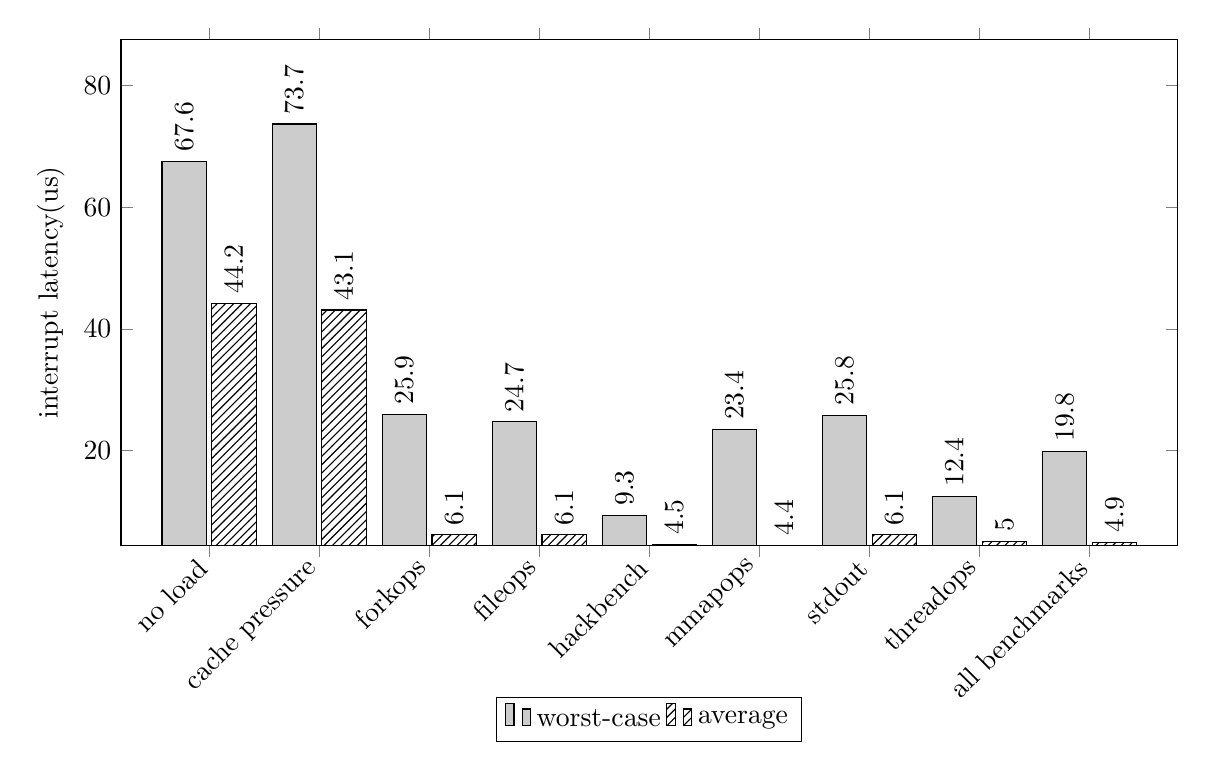
\begin{tikzpicture} %[scale=1.2]

\begin{axis} [ ybar=2pt, height=8cm, width=15cm, enlarge y limits={upper,value=0.2}, %enlargelimits=0.1,
                       legend style={at={(0.5,-0.3)}, anchor=north, legend columns=-1},
                       ylabel={interrupt latency(us)}, %title=vmexits after bootup, 
		       bar width=16pt,
       		       %%enlarge x limits={abs=0.8cm}, 		       
                       symbolic x coords={no load, cache pressure,forkops, fileops, hackbench, mmapops, stdout, threadops, all benchmarks},
                       xtick=data, nodes near coords, 
		       %nodes near coords align={vertical},
			%ymajorgrids=true, grid style = very thin,
		       every node near coord/.append style={rotate=90, anchor=west},
                       x tick label style={rotate=45,anchor=east}, ]                    

	\addplot [fill=black!20] coordinates {
				(no load, 67.6)				
				(cache pressure, 73.7)
				(forkops, 25.9)
				(fileops, 24.7)
				(hackbench, 9.3)
				(mmapops, 23.4)
				(stdout, 25.8)
				(threadops, 12.4)		
				(all benchmarks, 19.8)				
			    };

	\addplot [postaction={pattern=north east lines}] coordinates {
				(no load, 44.2)
				(cache pressure, 43.1)
				(forkops, 6.1)
				(fileops, 6.1)
				(hackbench, 4.5)
				(mmapops, 4.4)
				(stdout, 6.1)
				(threadops, 5.0)
				(all benchmarks, 4.9)		
			    };

\legend{worst-case, average}
\end{axis}

\end{tikzpicture}
\end{center}
\ifreport
\caption{Baseline Interrupt Latency}
\fi
\label{plot-baseline}
\end{figure}


The baseline worst-case and average interrupt latency histogram is plotted in Figure \ref{plot-baseline}.
The worst-case latency without load is about three times more than interrupt latency with load. 
One straightforward reason for lower latency with benchmarks is warming up of caches.
When benchmarks are running they exercise kernel library operations that warm up the caches. 
As a results, most memory access are satisfied from caches when external interrupt arrives.
An exception to this behavior is worst-case latency with \mcachepressure{} benchmark.
This time the caches are polluted by the benchmark, resulting in increased overhead to service an interrupt.
The average-case latency follows same trend, when caches are warmed-up the average case is about $5$ times lower than the worst-case.

\section{Virtualization overhead of PHIDIAS} \label{sec:virtual-overhead}
The latency measurement procedure is repeated for the rt-guest 
executing in a virtual machine to determine virtualization overhead for Phidias hypervisor.
The virtualized setup consists of rt-guest and gp-guest assigned to separated cores of the processor.
Both guests has virtualized LAPIC, LAPIC-Timer, IOAPIC, and UART.
The guest physical memory is limited to $256MB$ and LLC is shared.
Rt-guest has direct access to  PCIe GPIO device, 
but interrupts are received by Phidias hypervisor first and then routed to the rt-guest.
Figure \ref{fig-virtual} shows virtual setup used to measure virtualization overhead.
Furthermore, the rt-guest has direct access to HPET device. 
The HPET device is used by guest kernel as clock-source.

\begin{figure}[!htb]
\begin{center}
\begin{tikzpicture}

%\node at (0,5.625) [rectangle, draw=black, thick, fill=white, rounded corners, minimum height = 3cm, minimum width = 4cm, text width=2cm, anchor=south west] (rtguest) {};

\node at (0,2.25) [rectangle, draw=black, thick, fill=white, rounded corners, minimum height = 6cm, minimum width = 5cm, anchor=south west] (rtguest) {};

%\node[inner sep=0pt, text width=3cm] (rtgtext) at (2, 8) {PREEMPT\_RT guest};
%\node[inner sep=0pt] (tux) at (3, 7)  {
\includegraphics[width=1.5cm]{figures/tux.jpg}};
\node[below right, inner sep=5pt, text width=2cm] at (rtguest.north west) {PREEMPT\_RT\\ Linux\\ (rt-guest)};
\node[below left, inner sep=2pt] (tux1) at (rtguest.north east)  {
\includegraphics[width=1.8cm]{figures/tux.jpg}};


\node at (0.5,5.1) [rectangle, draw=black, thick, fill=black!5, rounded corners, minimum height = 0.8cm, minimum width = 4cm, anchor=south west] (vcpu1) {vCPU};
\node at (0.5,4.2) [rectangle, draw=black, thick, fill=black!5, rounded corners, minimum height = 0.8cm, minimum width = 1.9cm, anchor=south west] (vlapic1) {vLAPIC};
\node at (2.5,4.2) [rectangle, draw=black, thick, fill=black!5, rounded corners, minimum height = 0.8cm, minimum width = 2cm, anchor=south west] (vioapic1) {vIOAPIC};
\node at (0.5,3.2) [rectangle, draw=black, thick, fill=black!5, rounded corners, minimum height = 0.8cm, minimum width = 1.9cm, anchor=south west] (vdevice) {vTimer};
\node at (2.5,3.2) [rectangle, draw=black, thick, fill=black!5, rounded corners, minimum height = 0.8cm, minimum width = 2cm, anchor=south west] (vuart1) {vUART};

\node at (0.5,2.25+0.1) [rectangle, draw=black, thick, fill=black!10, rounded corners, minimum height = 0.7cm, minimum width = 4cm, anchor=south west] (vdevice) {\small{PCIe GPIO Device}};

\node at (0,1) [rectangle, draw=black, thick, fill=black!3, rounded corners, minimum height = 1cm, minimum width = 5cm, anchor=south west] (phidias1) {PHIDIAS};
\node at (0,0-0.125) [rectangle, draw=black, thick, fill=black!3, rounded corners, minimum height = 1cm, minimum width = 5cm, anchor=south west] (core0) {Core0};


\draw[black, thick, dashed] (5.25,-0.25) -- (5.25,9); %node at (0,0) [below] {release time};

\node at (5.5,2.25) [rectangle, draw=black, thick, fill=white, rounded corners, minimum height = 6cm, minimum width = 5cm, anchor=south west] (guest) {};
%\node[inner sep=0pt, text width=3cm] (rtgtext) at (7, 8) {guest2};
%\node[inner sep=0pt] (tux) at (7.5, 7)  {
\includegraphics[width=1.5cm]{figures/tux.jpg}};

\node[below right, inner sep=5pt, text width=2cm] at (guest.north west) {Linux\\ (gp-guest)};
\node[below left, inner sep=2pt] (tux2) at (guest.north east)  {
\includegraphics[width=1.8cm]{figures/tux.jpg}};

\node at (6,5.1) [rectangle, draw=black, thick, fill=black!5, rounded corners, minimum height = 0.8cm, minimum width = 4cm, anchor=south west] (vcpu2) {vCPU};
\node at (6,4.2) [rectangle, draw=black, thick, fill=black!5, rounded corners, minimum height = 0.8cm, minimum width = 1.9cm, anchor=south west] (vlapic2) {vLAPIC};

\node at (8,4.2) [rectangle, draw=black, thick, fill=black!5, rounded corners, minimum height = 0.8cm, minimum width = 2cm, anchor=south west] (vioapic2) {vIOAPIC};
\node at (6,3.2) [rectangle, draw=black, thick, fill=black!5, rounded corners, minimum height = 0.8cm, minimum width = 1.9cm, anchor=south west] (vdevice) {vTimer};
\node at (8,3.2) [rectangle, draw=black, thick, fill=black!5, rounded corners, minimum height = 0.8cm, minimum width = 1.9cm, anchor=south west] (vuart2) {vUART};

\node at (5.5,1) [rectangle, draw=black, thick, fill=black!3, rounded corners, minimum height = 1cm, minimum width = 5cm, anchor=south west] (phidias2) {PHIDIAS};
\node at (5.5,0-0.125) [rectangle, draw=black, thick, fill=black!3, rounded corners, minimum height = 1cm, minimum width = 5cm, anchor=south west] (core1) {Core1};


\draw[black, thick, dotted] (-0.25, 2.1) -- (11,2.1);

\end{tikzpicture}
\end{center}
\ifreport
\caption{Virtual Setup used to measure virtualization overhead}
\fi
\label{fig-virtual}
\end{figure}

%%\begin{figure}[!htb]
\begin{center}
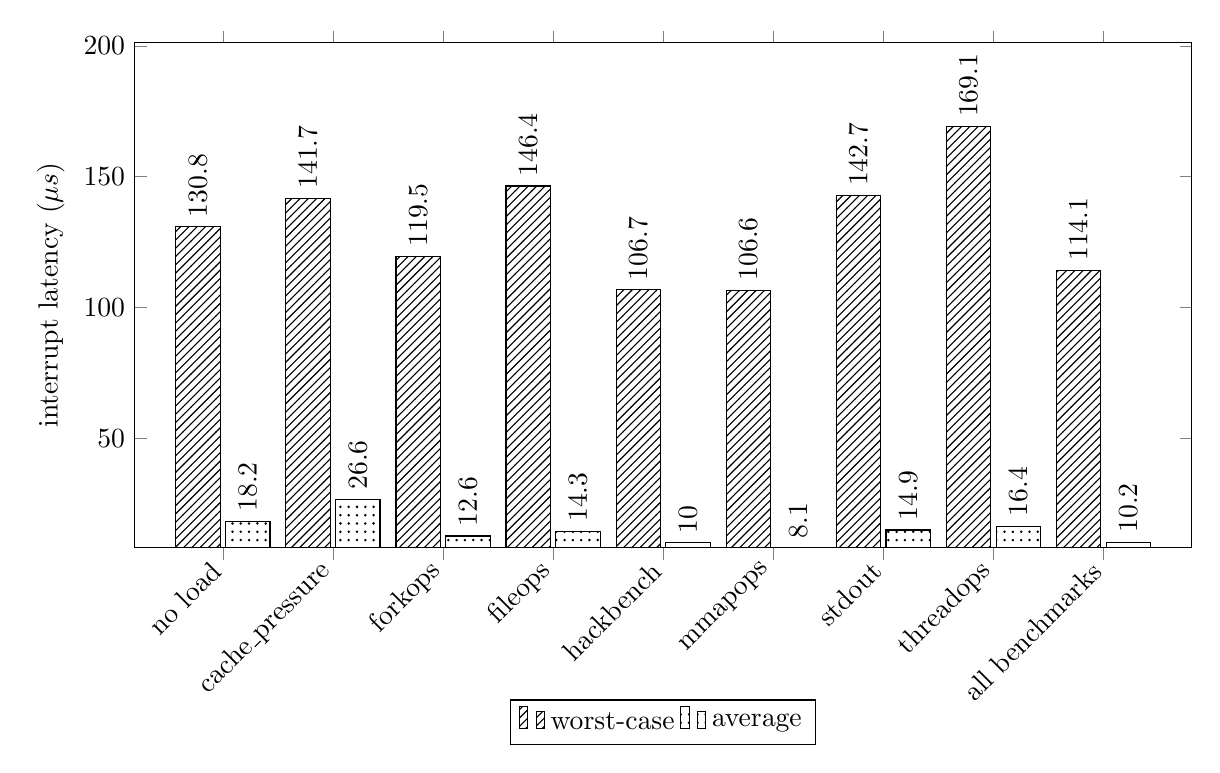
\begin{tikzpicture}

\begin{axis} [ ybar=2pt, height=8cm, width=15cm, enlarge y limits={upper,value=0.2}, %enlargelimits=0.1,
                       legend style={at={(0.5,-0.3)}, anchor=north, legend columns=-1}, 
                       ylabel={interrupt latency ($\mu{}s$)}, %title=vmexits after bootup, 
		       bar width=16pt,
       		       %%enlarge x limits={abs=0.8cm}, 		       
                       symbolic x coords={no load, cache\_pressure,forkops, fileops, hackbench, mmapops, stdout, threadops, all benchmarks},
                       xtick=data, nodes near coords, 
		       %nodes near coords align={vertical},
		       every node near coord/.append style={rotate=90, anchor=west},
                       x tick label style={rotate=45,anchor=east},]                    
	\addplot [postaction={pattern=north east lines}] coordinates {
				(no load, 130.8)
				(cache\_pressure, 141.7)
				(forkops, 119.5)
				(fileops, 146.4)
				(hackbench, 106.7)
				(mmapops, 106.6)
				(stdout, 142.7)
				(threadops, 169.1)				
				(all benchmarks, 114.1)				
			    };

	\addplot [postaction={pattern=dots}] coordinates {
				(no load, 18.2)
				(cache\_pressure, 26.6)
				(forkops, 12.6)
				(fileops, 14.3)
				(hackbench, 10)
				(mmapops, 8.1)
				(stdout, 14.9)
				(threadops, 16.4)				
				(all benchmarks, 10.2)				
			    };

\legend{worst-case, average}
\end{axis}

\end{tikzpicture}
\end{center}
\ifreport
\caption{Interrupt Latency in virtual setup}
\fi
\label{plot-virtual-overhead}
\end{figure}

\begin{figure}[!htb]
\begin{center}
\begin{tikzpicture}

\begin{axis} [name=plot1, height=\figheight, width=\figwidth, ybar=\ybarSepVO, enlarge y limits={upper,value=0.3},  
			ymin=0,
			legend pos=north east, legend columns=-1,
            ylabel={worst-case interrupt latency ($\mu{}s$)}, 
		    bar width=\ybarWidthVO,
			x=\ybarXdistVO,
            symbolic x coords={no load, cache\_pressure,forkops, fileops, hackbench, mmapops, stdout, threadops, all benchmarks},
            xtick=data, nodes near coords, nodes near coords align={vertical}, nodes near coords style={font=\ttfamily\scriptsize},
			x tick label style={rotate=25,anchor=east, font=\ttfamily\small}, ]                    
	\addplot [fill=yellow!20, postaction={pattern=north east lines}, pattern color=gray] coordinates {
				(no load, 67.6)				
				(cache\_pressure, 73.7)
				(forkops, 25.9)
				(fileops, 24.7)
				(hackbench, 9.3)
				(mmapops, 23.4)
				(stdout, 25.8)
				(threadops, 12.4)
				(all benchmarks, 19.8)
			      };

	\addplot [fill=NavyBlue!40] coordinates {
				(no load, 130.8)				
				(cache\_pressure, 141.7)
				(forkops, 119.5)
				(fileops, 146.4)
				(hackbench, 106.7)
				(mmapops, 106.6)
				(stdout, 142.7)
				(threadops, 169.1)
				(all benchmarks, 114.1)
			      };
\legend{native setup, virtual setup}
\end{axis}

%%%%%%%%%%%%%%%%%%for defense presentation%%%%%%%%%%%%%%%%%%%%
\ifdefense

\end{tikzpicture}
\end{center}
\label{plot-native-vs-virtual1}
\end{figure}
	
\begin{figure}[!htb]
\begin{center}
\begin{tikzpicture}

\fi
%%%%%%%%%%%%%%%%%%%%%ENDIF%%%%%%%%%%%%%%%%%%%%%%%%%%%%%%%%%

\begin{axis} [name=plot2,\atCmdVOverheadLowerPlot,  height=\figheight, width=\figwidth, ybar=\ybarSepVO, enlarge y limits={upper,value=0.2}, 
				ymin=0,
                legend pos=north east, legend columns=-1,
                ylabel={average-case interrupt latency ($\mu{}s$)}, 
		       	bar width=\ybarWidthVO,
				x=\ybarXdistVO,
				symbolic x coords={no load, cache\_pressure,forkops, fileops, hackbench, mmapops, stdout, threadops, all benchmarks},
                xtick=data, nodes near coords, nodes near coords align={vertical},  nodes near coords style={font=\ttfamily\scriptsize},
				 x tick label style={rotate=25,anchor=east, font=\ttfamily\small}, ]                    
	\addplot [fill=yellow!20, postaction={pattern=north east lines}, pattern color=gray] coordinates {
				(no load, 44.2)				
				(cache\_pressure, 43.1)
				(forkops, 6.1)
				(fileops, 6.1)
				(hackbench, 4.5)
				(mmapops, 4.4)
				(stdout, 6.1)
				(threadops, 5)
				(all benchmarks, 4.9)
			      };
	\addplot [fill=NavyBlue!40] coordinates {
				(no load, 18.2)				
				(cache\_pressure, 26.6)
				(forkops, 12.6)
				(fileops, 14.3)
				(hackbench, 10)
				(mmapops, 8.1)
				(stdout, 14.9)
				(threadops, 16.4)
				(all benchmarks, 10.2)
			      };
\legend{native setup, virtual setup}
\end{axis}

\end{tikzpicture}
\end{center}
\ifreport
\caption{Comparison of worst-case and average-case latency in native and virtual setup}
\label{plot-native-vs-virtual}
\else
\label{plot-native-vs-virtual2}
\fi
\end{figure}


Figure \ref{plot-native-vs-virtual} plots comparison of worst-case and average-case latency in native and virtual setup.
The worst-case interrupt latency of virtualized rt-guest has increased more than twice for all microbenchmarks.
However, considering the worst-case scenario for native setup, the increase is about $2$ times when loaded with \mcachepressure{} benchmark.
Worst-case latency is affected more than the average-case latency in virtualized environment.

On average virtualization has increased interrupt latency by an offset of $100\mu{}s$.
The increased interrupt response time demands in-depth investigation of each overhead component which is covered in section \ref{sec:overheadcomp}.
Figure \ref{plot-cdf-native-vs-virtual} plots CDF (cumulative density function) of latency in native and virtual setups for three load conditions.
The CDF in virtual setup almost always follows the native pattern.
The patterns reveal that in virtual setup the interrupt latency is shifted by an offset which is approximately the difference in average-case latency.
The probability of worst-case interrupt latency is very low and most events converge to the average-case.

\begin{figure}[!htb]
\begin{center}

\begin{tikzpicture}


\begin{axis}[name=plot1, height=6cm, width=12cm, ymin=0, ymax=1, xmin=0, 		
		xlabel=latency(us), 
		ylabel=probability,
		title style={yshift=-2ex},
		legend pos=south east,
		title=load:cache pressure,
		]
	\addplot [thick, blue] table[x=Latency,y=Probability] {./figures/native_cachepressure_10k_cdf.dat};
	\addplot [thick, red] table[x=Latency,y=Probability] {./figures/virt_cachepressure_10k_cdf.dat};
	\legend {\small{native (max 77.9)}, \small{virtual (max 131.1)}}
\end{axis}


\begin{axis}[name=plot2, at={($(plot1.south west)+(0,-6.5cm)$)}, height=6cm, width=12cm, ymin=0, ymax=1, xmin=0, 
		legend pos=south east,
		xlabel=latency(us), 
		ylabel=probability, 
		title style={yshift=-2ex},
		title=load:threadops,
		]
	\addplot [thick, blue] table[x=Latency,y=Probability] {./figures/native_threadops_cdf.dat};	
	\addplot [thick, red] table[x=Latency,y=Probability] {./figures/virt_threadops_10k_cdf.dat};
	\legend {\small{native (max 12.4)}, \small{virtual (max 169.1)}}
\end{axis}



\begin{axis}[name=plot3, at={($(plot2.south west)+(0,-6.5cm)$)}, height=6cm, width=12cm, ymin=0, ymax=1, xmin=0, 
		legend pos=south east,
		xlabel=latency(us), 
		ylabel=probability, 
		title style={yshift=-2ex},
		title=load:forkops,
		]
	\addplot [thick, blue] table[x=Latency,y=Probability] {./figures/native_forkops_10k_cdf.dat};	
	\addplot [thick, red] table[x=Latency,y=Probability] {./figures/virt_forkops2_10k_cdf.dat};
	\legend {\small{native (max 25.9)}, \small{virtual (max 119.5)}}
\end{axis}

\end{tikzpicture}
\end{center}
\caption{Comparison of interrupt latency CDF between native and virtual setup for different load conditions}
\label{plot-cdf-native-vs-virtual}
\end{figure}


Before moving on it is important to investigate how often Hypervisor intervention is required by the guest code.
Next section reports guest traps recorded for the duration of an experiment with different load conditions.


\subsection{Phidias Intervention}
A key aspect to lower virtualization overhead is to keep hypervisor intervention to a minimum and allow guest code to execute directly on the processor.
This section records frequency at which guest is trapped to hypervisor.
A small instrumentation code was inserted in hypervisor exit handler routine to measure number of exits for the duration of an experiment. 
Figure \ref{plot-phidias-inter} plots frequency of exits during each experiment. 
Execution of an experiment with a load condition took about $30s$.
\begin{figure}[!htbp]
\begin{center}
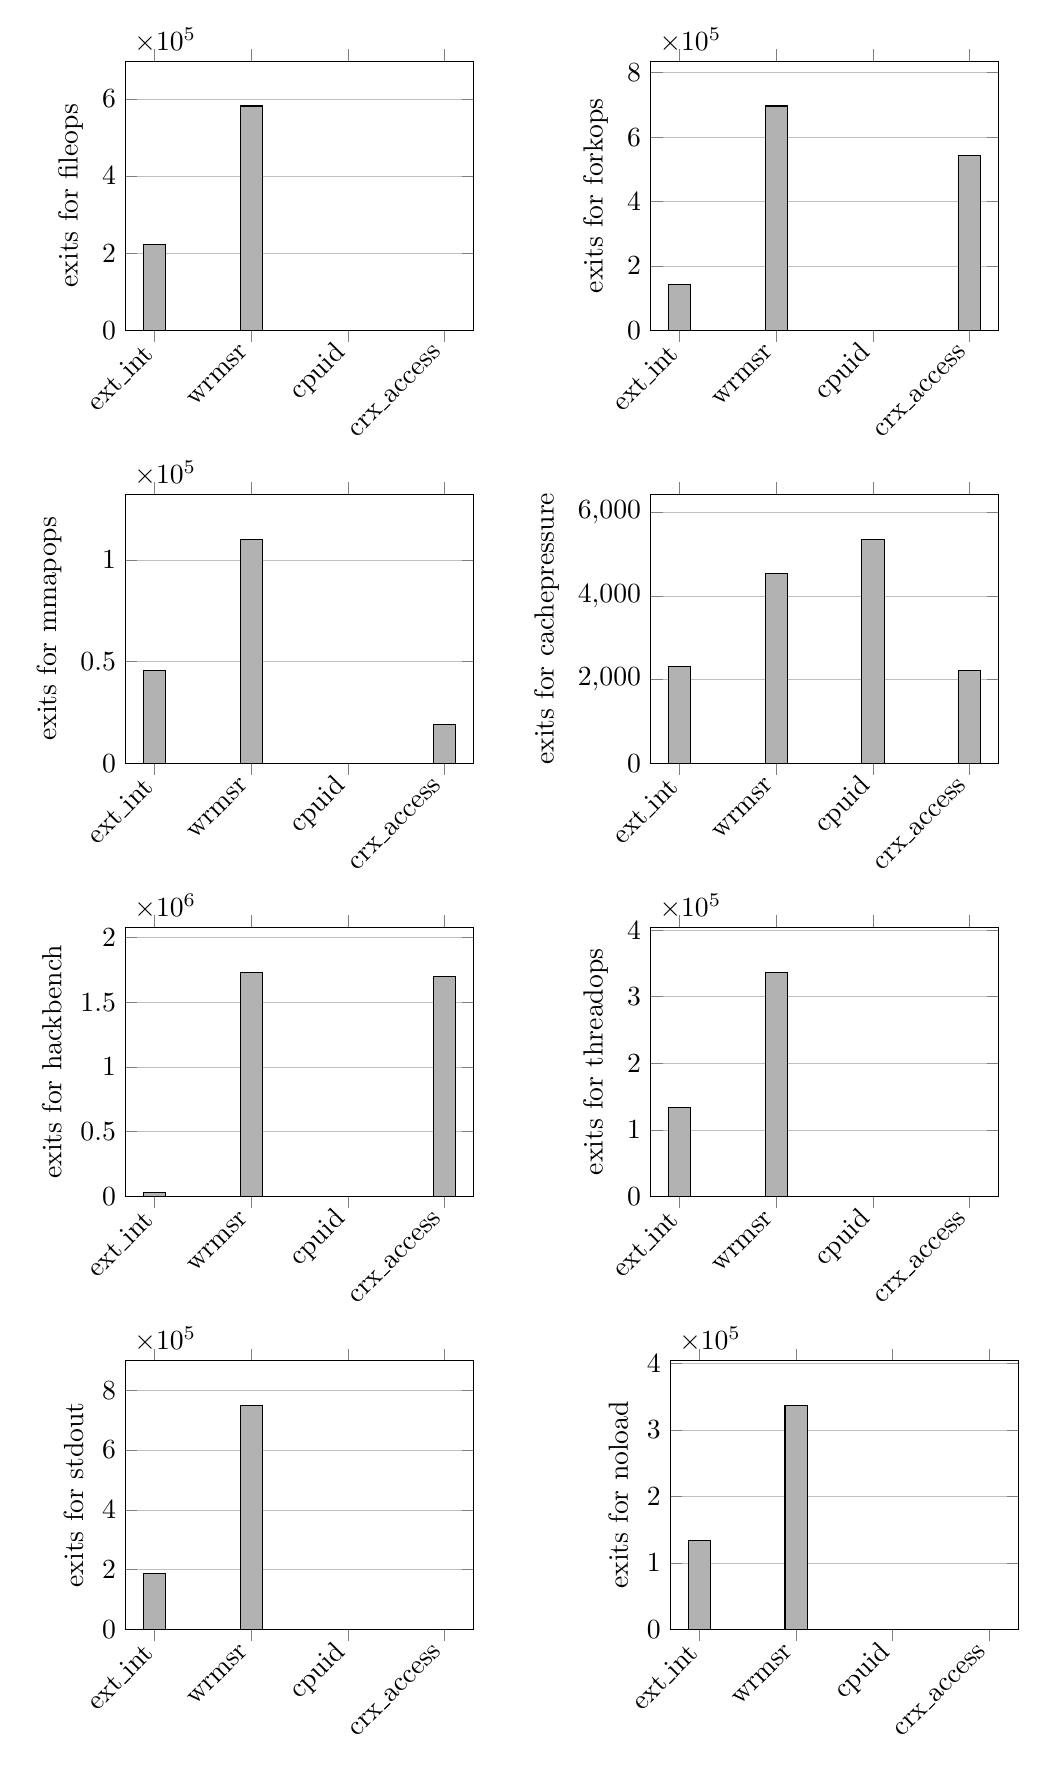
\begin{tikzpicture}


	\begin{axis} [name=plot1, ymin=0, ybar=2pt, height=5cm, width=6cm, enlarge y limits={upper,value=0.2}, 
		       legend style={at={(0.5,-0.3)}, anchor=north, legend columns=-1},
               ylabel={exits for fileops},
		       bar width=8pt,       
               symbolic x coords={ext\_int, wrmsr, cpuid, crx\_access},
               %xtick=data, nodes near coords, 
		       %nodes near coords align={vertical},
    		   ymajorgrids=true, grid style = very thin,
               x tick label style={rotate=45,anchor=east},]   

		\addplot [fill=black!30] coordinates {
				(ext\_int,222767)
				(wrmsr, 581681)
				(cpuid,0)
				(crx\_access,0)
			    };
	\end{axis}


	\begin{axis} [name=plot2, at={($(plot1.south east)+(2.25cm,0)$)}, ymin=0, ybar=2pt, height=5cm, width=6cm, enlarge y limits={upper,value=0.2}, 
		       legend style={at={(0.5,-0.3)}, anchor=east, legend columns=-1},
               ylabel={exits for forkops},
		       bar width=8pt,       
		symbolic x coords={ext\_int, wrmsr, cpuid, crx\_access},
               %xtick=data, nodes near coords, 
		       %nodes near coords align={vertical},
    		   ymajorgrids=true, grid style = very thin,
               x tick label style={rotate=45,anchor=east},]
		\addplot [fill=black!30] coordinates {
				(ext\_int,140981)
				(wrmsr, 696616)
				(cpuid,0)
				(crx\_access,543490)
			    };
	\end{axis}


	\begin{axis} [name=plot3, at={($(plot1.south west)+(0,-5.5cm)$)}, ymin=0, ybar=2pt, height=5cm, width=6cm, enlarge y limits={upper,value=0.2}, 
		       legend style={at={(0.5,-0.3)}, anchor=east, legend columns=-1},
               ylabel={exits for mmapops},
		       bar width=8pt,       
               symbolic x coords={ext\_int, wrmsr, cpuid, crx\_access},
               %xtick=data, nodes near coords, 
		       %nodes near coords align={vertical},
    		   ymajorgrids=true, grid style = very thin,
               x tick label style={rotate=45,anchor=east},]
		\addplot [fill=black!30] coordinates {
				(ext\_int,45641)
				(wrmsr, 110179)
				(cpuid,0)
				(crx\_access,18902)
			    };
	\end{axis}


	\begin{axis} [name=plot4, at={($(plot3.south east)+(2.25cm,0)$)}, ymin=0, ybar=2pt, height=5cm, width=6cm, enlarge y limits={upper,value=0.2}, 
		       legend style={at={(0.5,-0.3)}, anchor=east, legend columns=-1},
               ylabel={exits for cachepressure},
		       bar width=8pt,       
               symbolic x coords={ext\_int, wrmsr, cpuid, crx\_access},
               %xtick=data, nodes near coords, 
		       %nodes near coords align={vertical},
    		   ymajorgrids=true, grid style = very thin,
               x tick label style={rotate=45,anchor=east},]
		\addplot [fill=black!30] coordinates {
				(ext\_int,2319)
				(wrmsr, 4540)
				(cpuid,5358)
				(crx\_access,2208)
			    };
	\end{axis}


	\begin{axis} [name=plot5, at={($(plot3.south west)+(0,-5.5cm)$)}, ymin=0, ybar=2pt, height=5cm, width=6cm, enlarge y limits={upper,value=0.2}, 
		       legend style={at={(0.5,-0.3)}, anchor=east, legend columns=-1},
               ylabel={exits for hackbench},
		       bar width=8pt,       
               symbolic x coords={ext\_int, wrmsr, cpuid, crx\_access},
               %xtick=data, nodes near coords, 
		       %nodes near coords align={vertical},
    		   ymajorgrids=true, grid style = very thin,
               x tick label style={rotate=45,anchor=east},]
		\addplot [fill=black!30] coordinates {
				(ext\_int,31602)
				(wrmsr, 1731800)
				(cpuid,0)
				(crx\_access,1698102)
			    };
	\end{axis}


	\begin{axis} [name=plot6, at={($(plot5.south east)+(2.25cm,0)$)}, ymin=0, ybar=2pt, height=5cm, width=6cm, enlarge y limits={upper,value=0.2}, 
		       legend style={at={(0.5,-0.3)}, anchor=east, legend columns=-1},
               ylabel={exits for threadops},
		       bar width=8pt,       
               symbolic x coords={ext\_int, wrmsr, cpuid, crx\_access},
               %xtick=data, nodes near coords, 
		       %nodes near coords align={vertical},
    		   ymajorgrids=true, grid style = very thin,
               x tick label style={rotate=45,anchor=east},]
		\addplot [fill=black!30] coordinates {
				(ext\_int,133559)
				(wrmsr, 336922)
				(cpuid,0)
				(crx\_access,0)
			    };
	\end{axis}


	\begin{axis} [name=plot7, at={($(plot5.south west)+(0,-5.5cm)$)}, ymin=0, ybar=2pt, height=5cm, width=6cm, enlarge y limits={upper,value=0.2}, 
		       legend style={at={(0.5,-0.3)}, anchor=east, legend columns=-1},
               ylabel={exits for stdout},
		       bar width=8pt,       
               symbolic x coords={ext\_int, wrmsr, cpuid, crx\_access},
               %xtick=data, nodes near coords, 
		       %nodes near coords align={vertical},
    		   ymajorgrids=true, grid style = very thin,
               x tick label style={rotate=45,anchor=east},]
		\addplot [fill=black!30] coordinates {
				(ext\_int,187686)
				(wrmsr, 749643)
				(cpuid,0)
				(crx\_access,0)
			    };
	\end{axis}


	\begin{axis} [name=plot8, at={($(plot7.south east)+(2.5cm,0)$)}, ymin=0, ybar=2pt, height=5cm, width=6cm, enlarge y limits={upper,value=0.2}, 
		       legend style={at={(0.5,-0.3)}, anchor=east, legend columns=-1},
               ylabel={exits for noload},
		       bar width=8pt,       
               symbolic x coords={ext\_int, wrmsr, cpuid, crx\_access},
               %xtick=data, nodes near coords, 
		       %nodes near coords align={vertical},
    		ymajorgrids=true, grid style = very thin,
               x tick label style={rotate=45,anchor=east},]
		\addplot [fill=black!30] coordinates {
				(ext\_int,133559)
				(wrmsr, 336922)
				(cpuid,0)
				(crx\_access,0)
			    };
	\end{axis}

\end{tikzpicture}
\end{center}
\caption{Exit frequency with various load conditions for 30s duration}
\label{plot-phidias-inter}
\end{figure}


The plot categorizes exits on the basis of exit reason. 
The guest code is trapped to hypervisor more often than the rate at which external interrupts are sent to the real-time guest.
In worst-case guest is trapped 115 times in 1ms for experiment with \mhackbench{} load. About one time in best-case with \mcachepressure{} load.
When guest is trapped the hypervisor emulates the desired guest behavior. The emulation takes time and could cause pollution of shared resources like caches and TLBs. Emulation and resource contention are the main reason for increase in the interrupt response time.
Arrival of external interrupt, access to CR (control register) and write to an MSR(model specific register) are the most common reasons for exit.
In the next section each component of virtualization overhead is measured separately.


\subsection{Overhead Components} \label{sec:overheadcomp}
The virtualization overhead consists of four components. 
Figure \ref{fig-virt-overhead-all-comp} describes all overhead components.
First is the context switch times for vmexits and vmentries.
This overhead is experienced by every guest trap and it is purely hardware overhead.
Hardware-assisted virtualization extensions support context store and restore on vmexit and vmentry transitions.
The second overhead component is hypervisor run-time, which is emulation of desired behavior or routing of interrupts when guest is trapped.
This component can range from few machine cycles to thousands when no action is required to full device emulation.
The third component of the overhead is resource contention of shared resources like TLBs and LLC cache.
This component is variable and depends how much the guest and hypervisor cached enteries interfere with each other.
The last component is MMU virtualization which includes nested page-walks. 
As explained earlier in section \ref{sec:vmmu}, virtualized system uses nested page-tables to translate 
guest physical page numbers to machine physical page numbers. The nested paging involves higher number of pointer dereferences, which in turn
can significantly increase the memory access times for the guest code.
Phidias runtime and context-switch times can be measured by adding small instrumentation code in hypervisor and real-time guest. 

Overheads resulting from resource contention and MMU virtualization are hard to measure.
However presence of these overheads is a fact and hardware techniques can help to reduce them.
The next chapter will shed light on some of the techniques to lower resource-contention overhead.
Here I will present results of efforts made to measure Phidias run-time and context-switch times.

\begin{figure}[!htb]
\begin{center}
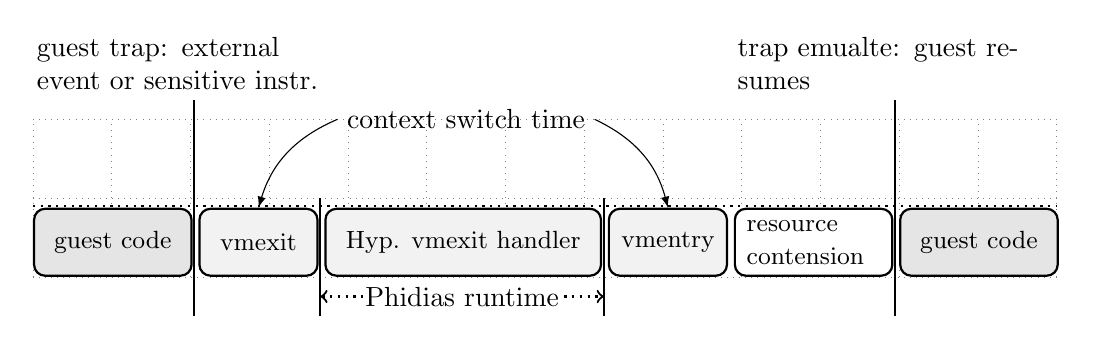
\begin{tikzpicture}

\newcommand\yh{0.85cm}

\draw[step=1cm, gray, very thin, dotted] (0,0) grid (13,2);
\draw[black, thick, dotted] (0,0.9) -- (13,0.9) node at (13,0.9) [below] {};

\node at (0,0) [rectangle, draw=black, thick, fill=black!10, rounded corners, minimum height = \yh, minimum width = 2cm, anchor=south west] (gcbefore) {\small{guest code}};
\node at (2.1,0) [rectangle, draw=black, thick, fill=black!5, rounded corners, minimum height = \yh, minimum width = 1.5cm, anchor=south west] (vmexit) {\small{vmexit}};
\node at (3.7,0) [rectangle, draw=black, thick, fill=black!5, rounded corners, minimum height = \yh, minimum width = 3.5cm, anchor=south west] (phidias) {\small{Hyp. vmexit handler}};
\node at (7.3,0) [rectangle, draw=black, thick, fill=black!5, rounded corners, minimum height = \yh, minimum width = 1.5cm, anchor=south west] (vmentry) {\small{vmentry}};

\node at (8.9,0) [rectangle, draw=black, thick, fill=white, rounded corners, minimum height = \yh, minimum width = 2cm, text width = 1.7cm, anchor=south west] (rc) {\small{resource\\ contension}};

\node at (11.0,0) [rectangle, draw=black, thick, fill=black!10, rounded corners, minimum height = \yh, minimum width = 2cm, anchor=south west] (gcafter) {\small{guest code}};

\draw[black, thick] (2.05,-0.5) -- (2.05, 2.25)  node [above, text width = 4cm] {guest trap: external event or sensitive instr.};
\draw[black, thick] (10.95,-0.5) -- (10.95, 2.25)  node [above, text width = 4cm] {trap emualte: guest resumes};

\draw[black, thick] (3.65,-0.5) -- (3.65, 1);
\draw[black, thick] (7.25,-0.5) -- (7.25, 1);
\draw[black, thick, dotted, <-] (3.65, -0.25) -- (4.25, -0.25); 
\draw[black, thick, dotted, ->] (6.75, -0.25) -- (7.25, -0.25);
\node at (5.45, -0.25) {Phidias runtime};

\node at (5.5, 2) (cslabel) [align=center] {context switch time};

\begin{scope}[>=latex]
	\draw [black, ->] (cslabel.west) to [bend right=25]  (vmexit.north);
	\draw [black, ->] (cslabel.east) to [bend left=25]  (vmentry.north);
\end{scope}

\end{tikzpicture}
\end{center}
\ifreport
\caption{Virtualization overhead components: Phidias runtime, context-switch time and resource contention}
\fi
\label{fig-virt-overhead-all-comp}
\end{figure}


\subsection{Phidias Runtime}
Phidias runtime is the time to emulate guest behavior for a trap. 
Phidias runtime can significantly influence interrupt latency and could be a major component of virtualization overhead.
Figure \ref{fig-virt-overhead-all-comp} shows Phidias runtime as the virtualization overhead component.

To measure Phidias runtime, a small instrumentation code was added at the beginning and end of Phidias vmexit handler.
The instrumentation code takes time-stamp at the beginning and end to measure worst-case vmexit handling time.
Furthermore, it also measures number of instructions executed for wort-case execution path using x86 performance monitoring core.
Figure \ref{plot-phidias-runtime} plots histogram of worst-case Phidias runtime to handle an exit. 

\begin{figure}[!htb]
\begin{center}
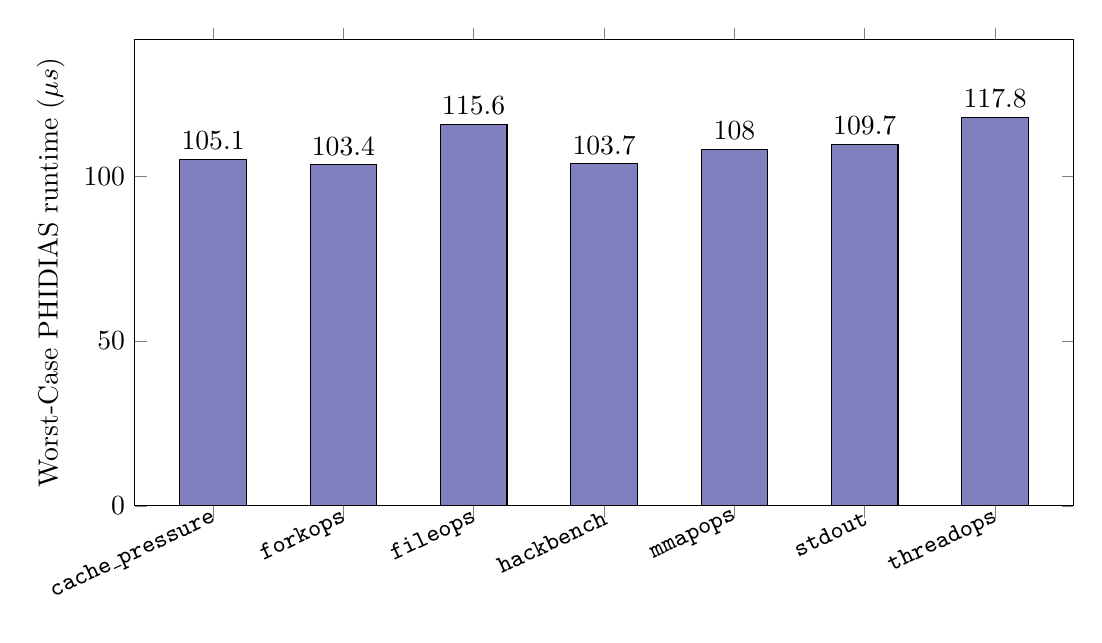
\begin{tikzpicture}

\begin{axis} [ ymin=0, ybar=2pt, height=7.5cm, width=\figwidth, enlarge y limits={upper,value=0.2}, 
		       legend style={at={(0.5,-0.3)}, anchor=north, legend columns=-1},
               ylabel={Worst-Case PHIDIAS runtime ($\mu{}s$)},
		       bar width=24pt,
  		       %%enlarge x limits={abs=0.8cm}, 		       
               symbolic x coords={no load, cache\_pressure,forkops, fileops, hackbench, mmapops, stdout, threadops, all benchmarks},
               xtick=data, nodes near coords, 
		       nodes near coords align={vertical},
		       %every node near coord/.append style={rotate=90, anchor=west},
               x tick label style={rotate=25, anchor=east, xshift=4pt, font=\ttfamily\small}, ]    

			\addplot [fill=NavyBlue!50] coordinates {				
				(cache\_pressure, 105.1)
				(forkops, 103.4)
				(fileops, 115.6)
				(hackbench, 103.7)
				(mmapops, 108)
				(stdout, 109.7)
				(threadops, 117.8)				
			    };
%\legend{}
\end{axis}

\end{tikzpicture}
\ifreport
\caption{Phidias runtime under different load conditions}
\fi
\end{center}
\label{plot-phidias-runtime}
\end{figure}


Table \ref{phidias-runtime} summarizes average and worst-case execution times of Phidias. It includes the number of
instructions executed during the worst-case path. To evaluate processor performance during the worst-case path CPI (cycles per instruction)
is calculated and enlisted in the table. 
In worst-case hypervisor code has CPI of $78$ clock cycles, which is too high.
Without any question, it can concluded that worst-case runtime is affected by resource contention.
The Phidias runtimes are taken from profiling information gathered during repeating
the latency measurement experiments. Detailed results are included in appendix \ref{app:b}.

\begin{table}[H]
\centering
\begin{longtable}{|c|c|c|c|c|}  
\hline
				& \multicolumn{2}{|c|}{Phidias run time} & instructions	& CPI\\
Benchmark		& average (cc)	&	worst-case (cc)	&	retired &	(WC) \\ \hline 
\mcachepressure{}	& 16548	& 178716 & 2322 & 77\\ \hline
\mforkops{}		& 9263 & 175702 & 2301 & 76.4\\ \hline
\mfileops{}		& 698 & 196490 & 12640 & 15.5\\ \hline
\mhackbench{} 		& 23042 & 176205 & 2301 & 76.6\\ \hline
\mmmapops{} 		& 7604 & 183566 & 2364 & 77.7\\ \hline
\mstdout{} 			& 1240 & 186435 & 21429 & 8.7\\ \hline
\mthreadops{} 		& 1265 & 200313 & 19804 & 10.1\\ \hline
\caption{Phidias worst-case execution time and CPU performance} 
\label{phidias-runtime}
\end{longtable}
\end{table}


\subsection{Context-Switch time} \label{sec:context-switch-overhead}
The context-switch time consists of hardware time needed for vmexit and vmentry.
In order to measure this overhead, a sensitive instruction was added to guest code to cause a trap. 
The instruction was wrapped in assertion and deassertion of an output pin, generating a pulse of the duration of instruction execution time.
Phidias was extended to return control back to guest code when trap is caused by the instruction added for trap.
External measurement setup explained earlier was used to measure context switch times for ten thousand traps.
The average and worst case times are summarized in table \ref{context-switch-time}.

\begin{table}[H]
\centering
\begin{longtable}{|c||c|c|}  
\hline
	Context-switch time	&	average (us)	&	worst-case (us) \\ \hline \hline
	\mnoload{}				&	1				&		17.2 \\ \hline
	\mcachepressure{}		&	1				&		86.8 \\ \hline
\caption{Context-switch overhead (hardware time to perform vmexit and vmentry)} 
\label{context-switch-time}
\end{longtable}
\end{table}

Context-switch time was measured in two scenarios. When there is no load on the guest
the worst-case context switch time is $17.2\mu{}s$. The experiment was repeated with \mcachepressure{} microbenchmark.
In worst-case this time can be as high as $86.8\mu{}s$ which is very close to virtualization overhead measured in the section \ref{sec:virtual-overhead}.
These results validate that most part of the virtualization overhead is made up of contention on the caches shared between guest and hypervisor.
Figure \ref{plot-cdf-contextswitch} plots CDF of context-switch times without load and with cache pressure.
The CDF is generated for 10,000 samples and shows that probability of high context-switch times than average values is very small.
\begin{figure}[!htb]
\begin{center}

\begin{tikzpicture}


\begin{axis}[name=plot1, height=8cm, width=12cm,
		legend pos=south east,
		xlabel=context-switch overhead ($\mu{}s$), 
		ylabel=Probability, enlargelimits=0.05,
		%ymajorgrids=true, grid style = very thin,
		]
	\addplot [ultra thick, blue] table[x=Latency,y=Probability] {./figures/vmexitentry_10k_cdf.dat};
	\addplot [very thick, red, dashed] table[x=Latency,y=Probability] {./figures/vmexitentry_cachepressure_10k_cdf.dat};
	\legend {\small{no load (max 17.2)}, \small{cache pressure (max 86.8)}}
\end{axis}

\end{tikzpicture}
\end{center}
\ifreport
\caption{CDF of context-switch overhead}
\fi
\label{plot-cdf-contextswitch}
\end{figure}


%%\subsection{Resource Contention}

%% \subsection{Purpose}
%%  This chapter will demonstrate virtualization overhead introduced by Phidias hypervisor.

%% Following topics are covered:
%% \begin {itemize}
%% \item overhead measurement mechanism and test setup
%% \item test scenarios (benchmarks)
%% \item test results and discussion 
%% \end {itemize}


%% \section{Latency Reduction}
%% \subsection{Purpose}
%% This chapter demonstrates results of latency reduction mechanisms

%% Following topics are covered:
%% \begin {itemize}
%% \item test enviorment and test scenarios
%% \item latency reduction using cache allocation technology 
%% \item latency reduction using direct interrupt injection
%% \item results and discussion
%% \end {itemize}

\chapter{Latency Reduction\label{chap4}}

Previous chapter demonstrated virtual interrupt latency for real-time guest is significantly larger than in native setup.
Recent extensions to x86 hardware-assisted virtualization support virtualization of local interrupt controller (APIC-v) 
that enables hypervisor to minimize its involvement. Furthermore, it allows direct interrupt injection to the guest for
devices that are owned by guests. It also enables virtualization of translation lookaside buffers (TLBs) by supporting virtual
process identifiers (VPIDs). Hypervisor can use VPIDs to isolate address translation information of different guests from each other and from hypervisor.
Intel Cache Allocation Technology addresses contention of shared LLC that enables hypervisor to partition shared cache
between the guests to avoid cache pollution.
This chapter presents results of using these hardware mechanisms to reduce interrupt latencies for real-time guest.
Following sections provide details of using each mechanism separately and records improvements in the interrupt latency.


\section{Direct Interrupt Injection}
Direct interrupt injection (DII) mechanism allows guest operating system to receive interrupts from 
external devices without hypervisor involvement.
APIC virtualization allows hypervisor to deliver virtual interrupts directly to the guest code without causing a trap. 
The details of this feature has already been covered in section \ref{sec:dii}.
A brief summary of the mechanism is as follows.
Hypervisor can marks a virtual interrupt as a posted interrupt (PI) in posted interrupt-descriptor (PID). 
PID is a data structure allocated by hypervisor.
It allows hypervisor inform interrupt controller that an interrupt is owned by guest and has to be delivered to guest without hypervisor involvement. 
Posted interrupt mechanism only works when hypervisor uses APIC virtualization to manage guest interrupts. 
Figure \ref{fig-posted-interrupts} demonstrates delivery of a guest interrupt does not require hypervisor involvement if it is marked as PI.
Succeeding sections describe performance evaluation of the real-time guest interrupt when DII is used.

\begin{figure}[!htb]
\begin{center}
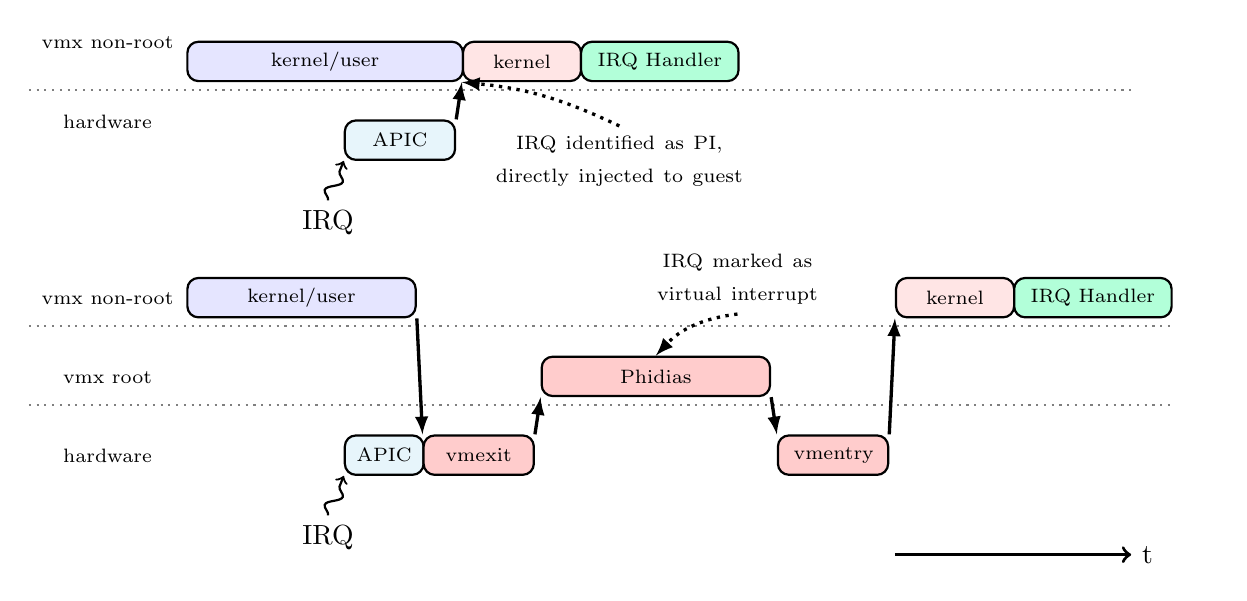
\begin{tikzpicture}

%\draw[step=1cm, gray, very thin, dotted] (-1,-1) grid (10,6);

\draw[black, very thick, ->] (9,-1) -- (12,-1) node [below, right] {t};
\draw[black, thick, dotted, opacity=0.5] (-2,0.9) -- (12.5,0.9) node at (13,0.9) [below] {};
\draw[black, thick, dotted, opacity=0.5] (-2,1.9) -- (12.5,1.9) node at (13,1.9) [below] {};
\node at (-1, 2.25) {\scriptsize{vmx non-root}};
\node at (-1, 1.25) {\scriptsize{vmx root}};
\node at (-1, 0.25) {\scriptsize{hardware}};


\node at (0,2) [rectangle, draw=black, thick, fill=Blue!10, rounded corners, minimum height = 0.5cm, minimum width = 2.9cm, anchor=south west] (kubefore) {\scriptsize{kernel/user}};
%\draw[black, thick, dashed, opacity=0.7] (1.95,-0.25) -- (1.95, 3.0)  node [above, text width = 1cm] {IRQ};
\node at (2,0) [rectangle, draw=black, thick, fill=SkyBlue!20, rounded corners, minimum height = 0.5cm, minimum width = 1cm, anchor=south west] (apic) {\scriptsize{APIC}};
%\draw[black, thick, dashed] (3.0,-0.25) -- (3.0, 3.75)  node [above, text width = 4cm] {IRQ not marked as PI};
\node at (3,0) [rectangle, draw=black, thick, fill=Red!20, rounded corners, minimum height = 0.5cm, minimum width = 1.4cm, anchor=south west] (vmexit) {\scriptsize{vmexit}};
\node at (4.5,1) [rectangle, draw=black, thick, fill=Red!20, rounded corners, minimum height = 0.5cm, minimum width = 2.9cm, anchor=south west] (phidias) {\scriptsize{Phidias}};
\node at (7.5,0) [rectangle, draw=black, thick, fill=Red!20, rounded corners, minimum height = 0.5cm, minimum width = 1.4cm, anchor=south west, text width=1cm] (vmentry) {\scriptsize{vmentry}};
%\draw[black, thick, dashed] (7.5,-0.25) -- (7.5, 3.25)  node [above, text width = 4cm] {IRQ marked pending};
\node at (9,2) [rectangle, draw=black, thick, fill=red!10, rounded corners, minimum height = 0.5cm, minimum width = 1.5cm, anchor=south west] (kafter) {\scriptsize{kernel}};
\node at (10.5,2) [rectangle, draw=black, thick, fill=SpringGreen!30, rounded corners, minimum height = 0.5cm, minimum width = 2cm, anchor=south west] (irqhandler) {\scriptsize{IRQ Handler}};
\draw[thick, decorate, decoration=snake, ->] (1.8, -0.5) -- (2, 0) node at (1.8, -0.5) [below] {IRQ};


\node at (7,2.5) (irqvi) [text width=4cm, align=center] {\scriptsize{IRQ marked as virtual interrupt}};
\node at (5.5,4) (irqpi) [text width=4cm, align=center] {\scriptsize{IRQ identified as PI, directly injected to guest}};

\begin{scope}[>=latex]
	%\draw [thick, ->] (kubefore.south east) to [bend right=0] (vmexit.north west);
	\draw [very thick, ->] (kubefore.south east) -- (vmexit.north west);
	\draw [very thick, ->] (vmexit.north east) -- (phidias.south west);
	\draw [very thick, ->] (phidias.south east) -- (vmentry.north west);
	\draw [very thick, ->] (vmentry.north east) -- (kafter.south west);
	\draw [very thick, dotted, ->] (irqvi.south) to [bend right=20] (phidias.north);
	
\end{scope}

\draw[black, thick, dotted, opacity=0.5] (-2,8-3.1) -- (12,8-3.1) node at (13,8-3.1) [below] {};
\node at (-1, 8-2.5) {\scriptsize{vmx non-root}};
\node at (-1, 8-3.5) {\scriptsize{hardware}};

\node at (0,8-3) [rectangle, draw=black, thick, fill=Blue!10, rounded corners, minimum height = 0.5cm, minimum width = 3.5cm, anchor=south west] (kubefore2) {\scriptsize{kernel/user}};
%\draw[black, thick, dashed, opacity=0.7] (1.95,-4.25) -- (1.95, -2.0)  node [above, text width = 1cm] {IRQ};
\draw[thick, decorate, decoration=snake, ->] (1.8, 8-4.5) -- (2, 8-4) node at (1.8, 8-4.5) [below] {IRQ};
\node at (2.0,8-4) [rectangle, draw=black, thick, fill=SkyBlue!20, rounded corners, minimum height = 0.5cm, minimum width = 1.4cm, anchor=south west] (apic2) {\scriptsize{APIC}};
%\draw[black, thick, dashed] (3.5,-4.25) -- (3.5, -1.5)  node [above, text width = 4cm] {IRQ recognized as PI};

\node at (3.5,8-3) [rectangle, draw=black, thick, fill=red!10, rounded corners, minimum height = 0.5cm, minimum width = 1.5cm, anchor=south west] (kafter2) {\scriptsize{kernel}};
\node at (5.0,8-3) [rectangle, draw=black, thick, fill=SpringGreen!30, rounded corners, minimum height = 0.5cm, minimum width = 2cm, anchor=south west] (irqhandler2) {\scriptsize{IRQ Handler}};

\begin{scope}[>=latex]
	\draw [very thick, ->] (apic2.north east) -- (kafter2.south west);
	\draw [very thick, dotted, ->] (irqpi.north) to [bend right=10] (kafter2.south west);
\end{scope}


\end{tikzpicture}
\end{center}
\ifreport
\caption{Posted interrupt versus virtual interrupt delivery}
\fi
\label{fig-posted-interrupts}
\end{figure}



\subsection{Methodology}
Performance evaluation setup for direct interrupt injection mechanism includes PREEMPT\_RT patched Linux as real-time guest (rt-guest)
and Linux as general-purpose guest (gp-guest). Each guest is assigned to a separate core and has access to 256MB of RAM. The setup is 
similar to the one described in section \ref{sec:methodology}, rt-guest has direct access to PCIe gpio card capable to generate interrupts. 
Measurement setup is same as described in section \ref{sec:measurement-setup}.
Phidias hypervisor was extended to use direct interrupt mechanism for rt-guest GPIO interrupt.
PID data structure has an outstanding notification (ON) bit that enables DII logic. 
The ON bit is cleared by hardware after injecting a posted interrupt directly to the guest. 
The hypervisor is responsible to set the bit again before arrival of posted interrupt, if it fails the interrupt is delivered to hypervisor.
Since external gpio interrupts events are generated at rate of about 1ms, hypervisor was informed by causing an intentional exit from interrupt handler to
set ON bit again. The approach is similar to the one used in section \ref{sec:context-switch-overhead}.
The latency reduction is evaluated by measuring worst-case interrupt latency with and without direct interrupt mechainsm.
It involves generating ten thousand GPIO interrupts and recording latency of each event.

\subsection{Latency Reduction}
\begin{figure}[!htb]
\begin{center}
\begin{tikzpicture} [
						my brace/.style={thick, decorate, decoration={brace, amplitude=4pt, raise=10pt,},},							
						my label/.style={below right, align=center, rotate=90, inner ysep=14pt, },						
					]

	%%%%%%% worst case %%%%%%%%%%%%%%
	\begin{axis} [ name=plot1, height=\figheight, width=\figwidth, 
				   enlarge y limits={upper,value=0.3},  enlarge x limits=0.12,
				   ymin=0,
		           %axis y line*=left,
				   ybar=\ybarSep,  
				   x=\ybarXdist,
				   bar width=\ybarWidth,
	   			   ylabel={worst-case interrupt latency ($\mu{}s$)},
	 		       symbolic x coords={no load, cache\_pressure, forkops, fileops, threadops},
		           xtick=data,                 
		            %nodes near coords, 
					%nodes near coords align={vertical}, 
					x tick label style={rotate=0, anchor=north, font=\ttfamily\small}, 
					%% xticklabel style={rotate=0,anchor=north},
		            xtick align=inside,
		            xticklabel pos=left,
	   			    legend pos=north east, legend columns=-1,
				]     
               
	\addplot [fill=yellow!20, postaction={pattern=north east lines}, pattern color=gray] coordinates {
				(no load, 67.6)				
				(cache\_pressure, 73.7)
				(forkops, 25.9)
				(fileops, 24.7)
				(threadops, 12.4)
		      };

	%% absolute values
	\addplot [fill=NavyBlue!50, xshift=\xShiftLatency] coordinates {
                    (no load,133.9) 
					(cache\_pressure,135.8)	
					(forkops,127.1)
					(fileops,127.6)
					(threadops,131.7)
			      }
					coordinate [pos=0] (a1)
		            coordinate [pos=0.2] (a2)
		            coordinate [pos=0.4] (a3)
		            coordinate [pos=0.8] (a4)
		            coordinate [pos=1] (a5)
				  ;

	\addplot [fill=ForestGreen!60, xshift=\xShiftLatency, postaction={pattern=crosshatch dots}, pattern color=gray] coordinates {
                    (no load,101.5) 
					(cache\_pressure,101.2)	
					(forkops,101.9)
					(fileops,101.1)
					(threadops,99.9)
			      }
				  	coordinate [pos=0] (b1)
		            coordinate [pos=0.2] (b2)
		            coordinate [pos=0.4] (b3)
		            coordinate [pos=0.8] (b4)
		            coordinate [pos=1] (b5)	
				  ;

				  \draw [my brace] (a1) -- (b1) node [my label] {\small{$+24.2\%$}};
				  \draw [my brace] (a2) -- (b2) node [my label] {\small{$+24.8\%$}};
				  \draw [my brace] (a3) -- (b3) node [my label] {\small{$+19.2\%$}};
				  \draw [my brace] (a4) -- (b4) node [my label] {\small{$+20.7\%$}};
				  \draw [my brace] (a5) -- (b5) node [my label] {\small{$+24.1\%$}};

	\legend{native, virtual interrupt, direct interrupt}
	\end{axis}

	%%improvement%%
	%% \begin{axis} [ name=plot1, height=\figheight, width=\figwidth, ybar,  enlarge y limits={upper,value=0.3},  enlarge x limits=0.12, 					
	%% 			   ymin=0, ymax=80,
	%% 	           axis y line*=right,
	%% 			   ybar=\ybarSep,  
	%% 			   x=\ybarXdist,
	%% 			   bar width=\ybarWidth,
	%%    			   ylabel={improvement \%},
	%%  		       symbolic x coords={no load, cache pressure, forkops, fileops, threadops},
	%% 	           xtick=data,                 
	%% 	            nodes near coords, 
	%% 				nodes near coords align={vertical}, 
	%% 				x tick label style={rotate=0, anchor=north}, 
	%% 				xticklabel style={rotate=0,anchor=north},
	%% 	            xtick align=inside,
	%% 	            xticklabel pos=left,
	%%    			    legend pos=north east, legend columns=-1,
	%% 	         ]  
	%% \addplot [fill=OliveGreen!50, xshift=\xShiftImprove, postaction={pattern=crosshatch dots}] coordinates {
    %%                 (no load,24.2) 
	%% 				(cache pressure,24.8)	
	%% 				(forkops,19.8)
	%% 				(fileops,20.7)
	%% 				(threadops,24.1)
	%% 		      };
	%% \legend{improvement}
	%% \end{axis}

%%%%%%% average case %%%%%%%%%%%%%%
%%%%%%%%%%%%%%%%%%for defense presentation%%%%%%%%%%%%%%%%%%%%
%%%%%%%%%%%%%%%%%%%%%IF%%%%%%%%%%%%%%%%%%%%%%%%%%%%%%%%%%%%%%%
\ifdefense

\end{tikzpicture}
\end{center}
\label{plot-dii1}
\end{figure}
	
\begin{figure}[!htb]
\begin{center}
\begin{tikzpicture} [
						my brace/.style={thick, decorate, decoration={brace, amplitude=4pt, raise=10pt,},},							
						my label/.style={below right, align=center, rotate=90, inner ysep=14pt, },
						label2/.style={below right, align=center, rotate=90, inner ysep=8pt, },
					]
%%%%%%%%%%%%%%%%%%%%%ENDIF%%%%%%%%%%%%%%%%%%%%%%%%%%%%%%%%%
\fi
	\begin{axis} [ name=plot2, \atCmdLowerPlot,  height=\figheight, width=\figwidth, enlarge y limits={upper,value=0.3},  enlarge x limits=0.12,
			   ymin=0,
               %axis y line*=left,
			   ybar=\ybarSep,
			   x=\ybarXdist,
		       bar width=\ybarWidth,
   			   ylabel={average-case interrupt latency ($\mu{}s$)},
 		       symbolic x coords={no load, cache\_pressure, forkops, fileops, threadops},
               xtick=data,                 
                %nodes near coords, 
				%nodes near coords align={vertical}, 
				x tick label style={rotate=0, anchor=north, font=\ttfamily\small}, 
				%% xticklabel style={rotate=0,anchor=north},
                xtick align=inside,
                xticklabel pos=left,
   			    legend pos=north east, legend columns=-1,
			]
	\addplot [fill=yellow!20, postaction={pattern=north east lines}, pattern color=gray] coordinates {
				(no load, 44.2)				
				(cache\_pressure, 43.1)
				(forkops, 6.1)
				(fileops, 6.1)
				(threadops, 5)
			   };  
              
	\addplot [fill=NavyBlue!50, xshift=\xShiftLatency] coordinates {
                    (no load,19.6) 
					(cache\_pressure,19.4)	
					(forkops,14)
					(fileops,15.1)
					(threadops,11.9)			
			      }
					coordinate [pos=0] (a1)
		            coordinate [pos=0.2] (a2)
		            coordinate [pos=0.4] (a3)
		            coordinate [pos=0.8] (a4)
		            coordinate [pos=1] (a5)
					;
	\addplot [fill=ForestGreen!60, xshift=\xShiftLatency, postaction={pattern=crosshatch dots}, pattern color=gray] coordinates {
                    (no load,11) 
					(cache\_pressure,11.4)	
					(forkops,8)
					(fileops,8)
					(threadops,11.3)			
 				    }
				  	coordinate [pos=0] (b1)
		            coordinate [pos=0.2] (b2)
		            coordinate [pos=0.4] (b3)
		            coordinate [pos=0.8] (b4)
		            coordinate [pos=1] (b5)	
					;

				  \draw [my brace] (a1) -- (b1) node [my label] {\small{$+43.8\%$}};
				  \draw [my brace] (a2) -- (b2) node [my label] {\small{$+41.2\%$}};
				  \draw [my brace] (a3) -- (b3) node [my label] {\small{$+42.9\%$}};
				  \draw [my brace] (a4) -- (b4) node [my label] {\small{$+47\%$}};
				  \draw [thick, |-|] ([xshift=12pt]a5) -- ([xshift=12pt]b5) node [xshift=-8pt, my label] {\small{$+5\%$}};

	\legend{native, virtual interrupt, direct interrupt}
	\end{axis}

	%%improvement%%
	%% \begin{axis} [ name=plot2, \atCmdLowerPlot,  height=\figheight, width=\figwidth, ybar,  
	%% 				enlarge y limits={upper,value=0.3},  enlarge x limits=0.12, ymin=0, ymax=80,
	%% 	           axis y line*=right,
	%% 			   ybar=\ybarSep,  
	%% 			   x=\ybarXdist,             
	%% 			   bar width=\ybarWidth,
	%%    			   ylabel={improvement \%},
	%%  		       symbolic x coords={no load, cache pressure, forkops, fileops, threadops},
	%% 	           xtick=data,                 
	%% 	            nodes near coords, 
	%% 				nodes near coords align={vertical}, 
	%% 				x tick label style={rotate=0, anchor=north}, 
	%% 				xticklabel style={rotate=0,anchor=north},
	%% 	            xtick align=inside,
	%% 	            xticklabel pos=left,
	%%    			    legend pos=north east, legend columns=-1,
	%% 	         ]  
	%% \addplot [fill=OliveGreen!50, xshift=\xShiftImprove, postaction={pattern=crosshatch dots}] coordinates {
    %%                 (no load,43.8) 
	%% 				(cache pressure,41.2)	
	%% 				(forkops,42.9)
	%% 				(fileops,47)
	%% 				(threadops,5)
	%% 		      };
	%% \legend{improvement}
	%% \end{axis}

\end{tikzpicture}
\end{center}
\ifreport
\caption{Interrupt Latency comparison for native, virtual and direct interrupt injection}
\label{plot-dii}
\else
\label{plot-dii2}
\fi
\end{figure}


The latency measurement experiment was repeated for different load conditions on real-time guest and no load on gp-guest. 
Figure \ref{plot-dii} plots comparison of worst-case and average-case interrupt latencies with and without DII. 
It is clear that direct interrupt injection reduces both worst-case and average-case interrupt latency. 
The best results are produced when guest is loaded with \mcachepressure{} benchmark. 
Interrupt latency reduced approximately by $33us$ with $25\%$ improvement.
%%All experiement resutls revealed that direct interrupt injection always reduces interrupt latencies.

%%\begin{figure}[!htb]
\begin{center}
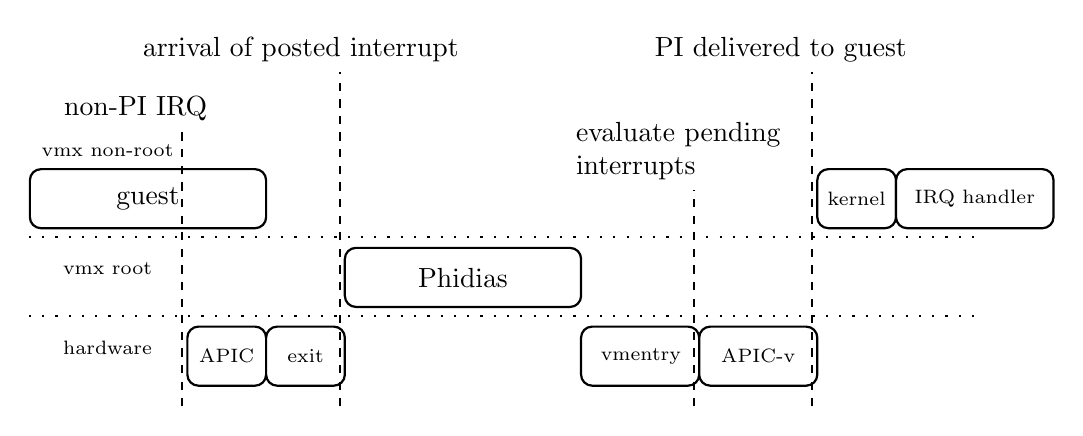
\begin{tikzpicture}

%\draw[step=1cm, gray, very thin, dotted] (0,0) grid (12,4);

\draw[black, thick, loosely dotted] (0,0.9) -- (12,0.9) node at (12,0.9) [below] {};
\draw[black, thick, loosely dotted] (0,1.9) -- (12,1.9) node at (12,1.9) [below] {};
\node at (1, 3) {\scriptsize{vmx non-root}};
\node at (1, 1.5) {\scriptsize{vmx root}};
\node at (1, 0.5) {\scriptsize{hardware}};


\node at (0,2) [rectangle, draw=black, thick, fill=white, rounded corners, minimum height = 0.75cm, minimum width = 3cm, anchor=south west] (gbefore) {guest};
\node at (2,0) [rectangle, draw=black, thick, fill=white, rounded corners, minimum height = 0.75cm, minimum width = 1cm, anchor=south west] (apic) {\scriptsize{APIC}};
\node at (3,0) [rectangle, draw=black, thick, fill=white, rounded corners, minimum height = 0.75cm, minimum width = 1cm, anchor=south west] (vmexit) {\scriptsize{exit}};
\node at (4,1) [rectangle, draw=black, thick, fill=white, rounded corners, minimum height = 0.75cm, minimum width = 3cm, anchor=south west] (phidias1) {Phidias};
\node at (7,0) [rectangle, draw=black, thick, fill=white, rounded corners, minimum height = 0.75cm, minimum width = 1.5cm, anchor=south west, text width=1cm] (entry) {\scriptsize{vmentry}};
\node at (8.5,0) [rectangle, draw=black, thick, fill=white, rounded corners, minimum height = 0.75cm, minimum width = 1.5cm, anchor=south west] (apicv) {\scriptsize{APIC-v}};

\draw[black, thick, dashed] (1.95,-0.25) -- (1.95, 3.25)  node [above, text width = 3cm] {non-PI IRQ};
\draw[black, thick, dashed] (3.95,-0.25) -- (3.95, 4.0)  node [above, text width = 5cm] {arrival of posted interrupt};
\draw[black, thick, dashed] (8.45,-0.25) -- (8.45, 2.5)  node [above, text width = 3cm] {evaluate pending interrupts};
\draw[black, thick, dashed] (9.95,-0.25) -- (9.95, 4.0)  node [above, text width = 4cm] {PI delivered to guest};

\node at (10,2) [rectangle, draw=black, thick, fill=white, rounded corners, minimum height = 0.75cm, minimum width = 1cm, anchor=south west] (gafter) {\scriptsize{kernel}};
\node at (11,2) [rectangle, draw=black, thick, fill=white, rounded corners, minimum height = 0.75cm, minimum width = 2cm, anchor=south west] (irqhandler) {\scriptsize{IRQ handler}};

\end{tikzpicture}
\end{center}
\caption{Posted interrupt worst case scenario}
\label{fig-pii-worstcase}
\end{figure}



\section{Portioning Last Level Cache}
Intel Cache Allocation Technology enables portioning of LLC (L3 cache).
The details of this feature has already been covered in section \ref{sec:cat}.
In short a set of registers called bitmasks allow hypervisor to configure isolated or shared cache regions.
A bit in the bitmask register can correspond to a way in set-associative cache.
A separate register is used to assign portion of the cache to an application based on an identifier called class of service (CLOS).
The Xeon E5-2600v4 processor used to conduct experiments has 15MB 20-way set associative cache bitmask registers has length of 20bits. 
It supports up to 15 CLOS identifiers.
Succeeding sections describe the methodology and records results of using cache allocation technique.


\subsection{Methodology}
The latency reduction is evaluated by measuring worst-case interrupt latency with and without LLC partitioning between the two guests.
The setup includes PREEMPT\_RT patched Linux as real-time guest (rt-guest)
and Linux as general-purpose guest (gp-guest). 
Each guest is assigned to a separate core and has access to 256MB of RAM.
The setup is similar to the one described in section \ref{sec:methodology}, rt-guest has direct access to PCIe gpio card capable to generate interrupts. 
Measurement setup is same as described in section \ref{sec:measurement-setup}.
Phidias hypervisor is extended to support portioning of L3 cache. 
The cache was divided equally between the two guests.
The gpio interrupt latency was measured while high memory demands were generate by gp-guest. 
The experiments were repeated with and without cache allocation to measure improvement in latency.
A synthetic application was used to generate high memory demands from gp-guest.

\subsection{Latency Reduction}
\begin{figure}[!htb]
\begin{center}
\begin{tikzpicture}  [
						my brace/.style={thick, decorate, decoration={brace, amplitude=2pt, raise=10pt,},},							
						my label/.style={below right, align=center, rotate=90, inner ysep=14pt, },
					]

		\begin{axis} [ name=plot1, height=\figheight, width=\figwidth, 
				   enlarge y limits={upper,value=0.3},  enlarge x limits=0.12,
				   ymin=0,
		           %axis y line*=left,
				   ybar=\ybarSep,  
				   x=\ybarXdist,
				   bar width=\ybarWidth,
	   			   ylabel={worst-case interrupt latency ($\mu{}s$)},
	 		       symbolic x coords={no load, cache\_pressure, forkops, fileops, threadops},
		           xtick=data,                 
		            %nodes near coords, 
					%nodes near coords align={vertical}, 
					x tick label style={rotate=0, anchor=north}, 
					xticklabel style={rotate=0,anchor=north, font=\ttfamily\small},
		            xtick align=inside,
		            xticklabel pos=left,
	   			    legend pos=north east, legend columns=-1,
				] 
		\addplot [fill=yellow!20, postaction={pattern=north east lines}, pattern color=gray] coordinates {
				(no load, 67.6)				
				(cache\_pressure, 73.7)
				(forkops, 25.9)
				(fileops, 24.7)
				(threadops, 12.4)
		      };                  

		\addplot [fill=NavyBlue!50, xshift=\xShiftLatency] coordinates {
                     (no load,141.3) 
					(cache\_pressure,132)	
					(forkops,129.9)
					(fileops,123.7)
					(threadops,146.1)
			      }
					coordinate [pos=0] (a1)
		            coordinate [pos=0.2] (a2)
		            coordinate [pos=0.4] (a3)
		            coordinate [pos=0.8] (a4)
		            coordinate [pos=1] (a5)
				  ;

		\addplot [fill=ForestGreen!60, xshift=\xShiftLatency, postaction={pattern=crosshatch dots}, pattern color=gray] coordinates {
                    (no load,120.4) 
					(cache\_pressure,112.2)	
					(forkops,108.4)
					(fileops,106.8)
					(threadops,116.9)
			      }				  	
					coordinate [pos=0] (b1)
		            coordinate [pos=0.2] (b2)
		            coordinate [pos=0.4] (b3)
		            coordinate [pos=0.8] (b4)
		            coordinate [pos=1] (b5)	
				  ;

				  \draw [my brace] (a1) -- (b1) node [my label] {\small{$+14.8\%$}};
				  \draw [my brace] (a2) -- (b2) node [my label] {\small{$+8.8\%$}};
				  \draw [my brace] (a3) -- (b3) node [my label] {\small{$+16.6\%$}};
				  \draw [my brace] (a4) -- (b4) node [my label] {\small{$+13.7\%$}};
				  \draw [my brace] (a5) -- (b5) node [my label] {\small{$+20.0\%$}};
		\legend{native, LLC shared, LLC partitioned}
		\end{axis}

		%%improvement%% 
		%% \begin{axis} [ name=plot1, height=\figheight, width=\figwidth, ybar,  enlarge y limits={upper,value=0.3},  enlarge x limits=0.12, 					
		%% 		   ymin=0, ymax=80,
		%%            axis y line*=right,
		%% 		   ybar=\ybarSep,  
		%% 		   x=\ybarXdist,
		%% 		   bar width=\ybarWidth,
	   	%% 		   ylabel={improvement \%},
	 	%% 	       symbolic x coords={no load, cache pressure, forkops, fileops, threadops},
		%%            xtick=data,                 
		%%             nodes near coords, 
		%% 			nodes near coords align={vertical}, 
		%% 			x tick label style={rotate=0, anchor=north}, 
		%% 			xticklabel style={rotate=0,anchor=north},
		%%             xtick align=inside,
		%%             xticklabel pos=left,
	   	%% 		    legend pos=north east, legend columns=-1,
		%%          ]  
		%% \addplot [fill=OliveGreen!50, xshift=\xShiftImprove, postaction={pattern=crosshatch dots}] coordinates {
        %%             (no load, 14.8) 
		%% 			(cache pressure,8.8)	
		%% 			(forkops,16.6)
		%% 			(fileops,13.7)
		%% 			(threadops,20)
		%% 	      };
		%% \legend{improvement}
		%% \end{axis}

%%%%%%%%%%%%%%%%%%for defense presentation%%%%%%%%%%%%%%%%%%%%
\ifdefense

\end{tikzpicture}
\end{center}
\label{plot-cat1}
\end{figure}
	
\begin{figure}[!htb]
\begin{center}
\begin{tikzpicture}  [
						my brace/.style={thick, decorate, decoration={brace, amplitude=2pt, raise=10pt,},},							
						my label/.style={below right, align=center, rotate=90, inner ysep=14pt, },
					]

\fi
%%%%%%%%%%%%%%%%%%%%%ENDIF%%%%%%%%%%%%%%%%%%%%%%%%%%%%%%%%%
	\begin{axis} [ name=plot2, \atCmdLowerPlot, 
					height=\figheight, width=\figwidth, enlarge y limits={upper,value=0.3},  
					enlarge x limits=0.12,
				   ymin=0,
		           %axis y line*=left,
				   ybar=\ybarSep,
				   x=\ybarXdist,
				   bar width=\ybarWidth,
	   			   ylabel={average-case interrupt latency ($\mu{}s$)},
	 		       symbolic x coords={no load, cache\_pressure, forkops, fileops, threadops},
		           xtick=data,                 
		            %nodes near coords, 
					%nodes near coords align={vertical}, 
					x tick label style={rotate=0, anchor=north, font=\ttfamily\small}, 
					xticklabel style={rotate=0,anchor=north},
		            xtick align=inside,
		            xticklabel pos=left,
	   			    legend pos=north east, legend columns=-1,
				 ] 
		\addplot [fill=yellow!20, postaction={pattern=north east lines}, pattern color=gray] coordinates {
				(no load, 44.2)				
				(cache\_pressure, 43.1)
				(forkops, 6.1)
				(fileops, 6.1)
				(threadops, 5)
			   };  
                   
		\addplot [fill=NavyBlue!50, xshift=\xShiftLatency] coordinates {
                    (no load,19.1) 
					(cache\_pressure,28.5)	
					(forkops,13.1)
					(fileops,13.8)
					(threadops,19.6)			
			      }
					coordinate [pos=0] (a1)
		            coordinate [pos=0.2] (a2)
		            coordinate [pos=0.4] (a3)
		            coordinate [pos=0.8] (a4)
		            coordinate [pos=1] (a5)
				  ;
		\addplot [fill=ForestGreen!60, xshift=\xShiftLatency, postaction={pattern=crosshatch dots}, pattern color=gray] coordinates {
                     (no load,15.7) 
					(cache\_pressure,15.2)	
					(forkops,9.9)
					(fileops,10)
					(threadops,12.4)			
			      }				  	
					coordinate [pos=0] (b1)
		            coordinate [pos=0.2] (b2)
		            coordinate [pos=0.4] (b3)
		            coordinate [pos=0.8] (b4)
		            coordinate [pos=1] (b5)	
				  ;

				  \draw [my brace] (a1) -- (b1) node [my label] {\small{$+17.8\%$}};
				  \draw [my brace] (a2) -- (b2) node [my label] {\small{$+46.6\%$}};
				  \draw [my brace] (a3) -- (b3) node [my label] {\small{$+24.4\%$}};
				  \draw [my brace] (a4) -- (b4) node [my label] {\small{$+27.5\%$}};
				  \draw [my brace] (a5) -- (b5) node [my label] {\small{$+36.7\%$}};
	\legend{native, LLC shared, LLC partitioned}
	\end{axis}

	%%improvement%%
	%% \begin{axis} [ name=plot2, \atCmdLowerPlot,  height=\figheight, width=\figwidth, ybar,  
	%% 				enlarge y limits={upper,value=0.3},  enlarge x limits=0.12, ymin=0, ymax=80,
	%% 	           axis y line*=right,
	%% 			   ybar=\ybarSep,  
	%% 			   x=\ybarXdist,             
	%% 			   bar width=\ybarWidth,
	%%    			   ylabel={improvement \%},
	%%  		       symbolic x coords={no load, cache pressure, forkops, fileops, threadops},
	%% 	           xtick=data,                 
	%% 	            nodes near coords, 
	%% 				nodes near coords align={vertical}, 
	%% 				x tick label style={rotate=0, anchor=north}, 
	%% 				xticklabel style={rotate=0,anchor=north},
	%% 	            xtick align=inside,
	%% 	            xticklabel pos=left,
	%%    			    legend pos=north east, legend columns=-1,
	%% 	         ]  
	%% \addplot [fill=OliveGreen!50, xshift=\xShiftImprove, postaction={pattern=crosshatch dots}] coordinates {
    %%                 (no load,17.8) 
	%% 				(cache pressure,46.6)	
	%% 				(forkops,24.4)
	%% 				(fileops,27.5)
	%% 				(threadops,36.7)
	%% 		      };
	%% \legend{improvement}
	%% \end{axis}

\end{tikzpicture}
\end{center}
\ifreport
\caption{Interrupt latency comparison of shared LLC and partitioned LLC}
\label{plot-cat}
\else
\label{plot-cat2}
\fi
\end{figure}


The latency measurement experiment was repeated for different load conditions on rt-guest when gp-guest was executed application large amounts of memory. 
Figure \ref{plot-cat} plots comparison of worst-case and average-case interrupt latencies when LLC is shared and when it is partitioned. 
It is clear that separating real-time guest cache from the other guest improves both worst-case and average-case interrupt response times.
The best results are observed when guest is loaded with \mforkops{} benchmark. 
Interrupt latency reduced approximately by $21us$ with $16\%$ improvement.

%\section{Isolating TLB Traffic}
\section{TLB Virtualization} \label{sec:vtlb-latency-red}
Translation lookaside buffers (TLBs) are used by the processor to cache virtual to physical address translations.
Modern architectures have  separate TLBs for instruction and data known as iTLB and dTLB respectively. 
In a virtual environment hypervisor and guest operating system access different virtual address spaces.
Caching translations of both address spaces at same TLB can result in thrashing translations of each other on context switch. 
Furthermore when a guest flushes TLB entries, it also flushes cached information for hypervisor address space.
Hypervisor can use TLB virtualization through VPIDs to isolate traffic of its own address space from the guests running in virtual machines.
This section evaluates performance improvement for interrupt response time by using VPIDs.

\subsection{Methodology}
Two guest setup from the previous section is used again, however this time hypervisor is extended to use VPID mechanism.
Hypervisor assigns a unique process identifier to each guest and emulates TLB flush instructions for the guest 
based on VPIDs. The guest is oblivious to VPID mechanism.
Note that performance evaluation is focused on isolating guest translations from hypervisor as both execute on the same core.
Since Phidias hypervisor uses multikernel approach the shared resources are at least used by hypervisor and the guest.

The latency reduction is evaluated by measuring worst-case interrupt latency with and without TLB virtualization.
The setup includes PREEMPT\_RT patched Linux as real-time guest (rt-guest)
and Linux as general-purpose guest (gp-guest). 
The setup is similar to the one described in section \ref{sec:methodology}, rt-guest has direct access to PCIe gpio card capable to generate interrupts. 
Measurement setup is same as described in section \ref{sec:measurement-setup}.
Hypervisor was extended to support TLB virtualization. 
It assigns a unique process identifier to each guest and emulates TLB flush instructions for the guest based on VPIDs.

\subsection{Latency Reduction}

\begin{figure}[!htb]
\begin{center}
\begin{tikzpicture}  [
						my brace/.style={thick, decorate, decoration={brace, amplitude=3pt, raise=4pt,},},							
						my label/.style={below right, align=center, rotate=90, inner ysep=10pt, },
						another label/.style={below right, align=center, rotate=90, inner ysep=5pt, },
					]

	\begin{axis} [ name=plot1, height=\figheight, width=\figwidth, 
				   enlarge y limits={upper,value=0.3},  enlarge x limits=0.12,
				   ymin=0,
		           %axis y line*=left,
				   ybar=\ybarSep,  
				   x=\ybarXdist,
				   bar width=\ybarWidth,
	   			   ylabel={worst-case  latency ($\mu{}s$)},
	 		       symbolic x coords={no load, cache\_pressure, forkops, fileops, threadops},
		           xtick=data,                 
		            %nodes near coords, 
					%nodes near coords align={vertical}, 
					x tick label style={rotate=0, anchor=north, font=\ttfamily\small}, 
					xticklabel style={rotate=0,anchor=north},
		            xtick align=inside,
		            xticklabel pos=left,
	   			    legend pos=north east, legend columns=-1,
				 ]                    
	\addplot [fill=NavyBlue!50, xshift=\xShiftLatency] coordinates {
                    (no load,129.5) 
					(cache\_pressure,145.6)	
					(forkops,128.2)
					(fileops,127.1)
					(threadops,169.6)
			      }
					coordinate [pos=0] (a1)
		            coordinate [pos=0.2] (a2)
		            coordinate [pos=0.4] (a3)
		            coordinate [pos=0.8] (a4)
		            coordinate [pos=1] (a5)
				  ;

	\addplot [fill=ForestGreen!60, xshift=\xShiftLatency, postaction={pattern=crosshatch dots}, pattern color=gray] coordinates {
                    (no load,130.5) 
					(cache\_pressure,131.7)	
					(forkops,124.8)
					(fileops,123.7)
					(threadops,148.8)
			      }
				  	coordinate [pos=0] (b1)
		            coordinate [pos=0.2] (b2)
		            coordinate [pos=0.4] (b3)
		            coordinate [pos=0.8] (b4)
		            coordinate [pos=1] (b5)	
				  ;

				  \draw [thick, |-|] ([xshift=4pt]a1) -- ([xshift=4pt]b1) node [another label] {\small{$-0.8\%$}};
				  \draw [thick, |-|] ([xshift=4pt]a2) -- ([xshift=4pt]b2) node [another label] {\small{$+9.5\%$}};
				  \draw [thick, |-|] ([xshift=4pt]a3) -- ([xshift=4pt]b3) node [another label] {\small{$+2.6\%$}};
				  \draw [thick, |-|] ([xshift=4pt]a4) -- ([xshift=4pt]b4) node [another label] {\small{$+2.7\%$}};
				  \draw [my brace] (a5) -- (b5) node [my label] {\small{$+12.2\%$}};
	\legend{shared TLB, isolated TLB}
	\end{axis}

	%%improvement%%
	%% \begin{axis} [ name=plot1, height=\figheight, width=\figwidth, ybar,  enlarge y limits={upper,value=0.3},  enlarge x limits=0.12, 					
	%% 			   ymin=0, ymax=80,
	%% 	           axis y line*=right,
	%% 			   ybar=\ybarSep,  
	%% 			   x=\ybarXdist,
	%% 			   bar width=\ybarWidth,
	%%    			   ylabel={improvement \%},
	%%  		       symbolic x coords={no load, cache pressure, forkops, fileops, threadops},
	%% 	           xtick=data,                 
	%% 	            nodes near coords, 
	%% 				nodes near coords align={vertical}, 
	%% 				x tick label style={rotate=0, anchor=north}, 
	%% 				xticklabel style={rotate=0,anchor=north},
	%% 	            xtick align=inside,
	%% 	            xticklabel pos=left,
	%%    			    legend pos=north east, legend columns=-1,
	%% 	         ]  
	%% 	\addplot [fill=OliveGreen!50, xshift=\xShiftImprove, postaction={pattern=crosshatch dots}] coordinates {
    %%                 (no load, 0) 
	%% 				(cache pressure,9.5)	
	%% 				(forkops,2.6)
	%% 				(fileops,2.7)
	%% 				(threadops,12.2)
	%% 		      };
	%% 	\legend{improvement}
	%% 	\end{axis}
%%%%%%%%%%%%%%%%%%for defense presentation%%%%%%%%%%%%%%%%%%%%
\ifdefense

\end{tikzpicture}
\end{center}
\label{plot-vpid1}
\end{figure}
	
\begin{figure}[!htb]
\begin{center}
\begin{tikzpicture} [
						my brace/.style={thick, decorate, decoration={brace, amplitude=3pt, raise=4pt,},},							
						my label/.style={below right, align=center, rotate=90, inner ysep=10pt, },
					]

\fi
%%%%%%%%%%%%%%%%%%%%%ENDIF%%%%%%%%%%%%%%%%%%%%%%%%%%%%%%%%%

		\begin{axis} [	 name=plot2, \atCmdLowerPlot, 
					height=\figheight, width=\figwidth, enlarge y limits={upper,value=0.3},  
					enlarge x limits=0.12,
				   ymin=10,
		           %axis y line*=left,
				   ybar=\ybarSep,
				   x=\ybarXdist,
				   bar width=\ybarWidth,
	   			   ylabel={average-case latency ($\mu{}s$)},
	 		       symbolic x coords={no load, cache\_pressure, forkops, fileops, threadops},
		           xtick=data,                 
		            %nodes near coords, 
					%nodes near coords align={vertical}, 
					x tick label style={rotate=0, anchor=north}, 
					xticklabel style={rotate=0,anchor=north, font=\ttfamily\small},
		            xtick align=inside,
		            xticklabel pos=left,
	   			    legend pos=north east, legend columns=-1,
					]                    
		\addplot [fill=NavyBlue!50, xshift=\xShiftLatency] coordinates {
                    (no load,18.2) 
					(cache\_pressure,18.1)	
					(forkops,12.6)
					(fileops,14.5)
					(threadops,17)			
			      }
					coordinate [pos=0] (a1)
		            coordinate [pos=0.2] (a2)
		            coordinate [pos=0.4] (a3)
		            coordinate [pos=0.8] (a4)
		            coordinate [pos=1] (a5)
				  ;
		\addplot [fill=ForestGreen!60, xshift=\xShiftLatency, postaction={pattern=crosshatch dots}, pattern color=gray] coordinates {
                    (no load,17) 
					(cache\_pressure,16.7)	
					(forkops,11.6)
					(fileops,13.4)
					(threadops,15.4)			
			      }
				  	coordinate [pos=0] (b1)
		            coordinate [pos=0.2] (b2)
		            coordinate [pos=0.4] (b3)
		            coordinate [pos=0.8] (b4)
		            coordinate [pos=1] (b5)	
				  ;

				  \draw [my brace] (a1) -- (b1) node [my label] {\small{$+6.5\%$}};
				  \draw [my brace] (a2) -- (b2) node [my label] {\small{$+7.7\%$}};
				  \draw [my brace] (a3) -- (b3) node [my label] {\small{$+7.9\%$}};
				  \draw [my brace] (a4) -- (b4) node [my label] {\small{$+7.5\%$}};
				  \draw [my brace] (a5) -- (b5) node [my label] {\small{$+9.4\%$}};
		\legend{shared TLB, isolated TLB}
		\end{axis}

	%%improvement%%
	%% \begin{axis} [ name=plot2, \atCmdLowerPlot,  height=\figheight, width=\figwidth, ybar,  
	%% 				enlarge y limits={upper,value=0.3},  enlarge x limits=0.12, ymin=0, ymax=80,
	%% 	           axis y line*=right,
	%% 			   ybar=\ybarSep,  
	%% 			   x=\ybarXdist,             
	%% 			   bar width=\ybarWidth,
	%%    			   ylabel={improvement \%},
	%%  		       symbolic x coords={no load, cache pressure, forkops, fileops, threadops},
	%% 	           xtick=data,                 
	%% 	            nodes near coords, 
	%% 				nodes near coords align={vertical}, 
	%% 				x tick label style={rotate=0, anchor=north}, 
	%% 				xticklabel style={rotate=0,anchor=north},
	%% 	            xtick align=inside,
	%% 	            xticklabel pos=left,
	%%    			    legend pos=north east, legend columns=-1,
	%% 	         ]  
	%% \addplot [fill=OliveGreen!50, xshift=\xShiftImprove, postaction={pattern=crosshatch dots}] coordinates {
    %%                 (no load,6.5)
	%% 				(cache pressure,7.7)	
	%% 				(forkops,7.9)
	%% 				(fileops,7.5)
	%% 				(threadops,9.4)
	%% 		      };
	%% \legend{improvement}
	%% \end{axis}

\end{tikzpicture}
\end{center}
\ifreport
\caption{Interrupt latency comparison of shared and isolated TLB between guest and Phidias}
\label{plot-vpid}
\else
\label{plot-vpid2}
\fi
\end{figure}



The latency measurement experiment was repeated for different load conditions on real-time guest and no load on gp-guest. 
Figure \ref{plot-vpid} plots comparison of worst-case and average-case interrupt latencies with shared and isolated TLBs for rt-guest and hypervisor. 
Results show that separating guest TLB using VPID mechanism has improved both the worst-case and average-case interrupt latencies.
The average-case interrupt latency has decreased by at least $1.1us$. The worst-case latency has slightly increased with no load condition,
however it has always decreased with load conditions. 
The best results are produced when guest is loaded with \mthreadops{} benchmark. 
Interrupt latency reduced by approximately $20us$ with $12\%$ improvement.

\section{Putting it Altogether}
This section records improvement in real-time interrupt latency when all latency reduction techniques are combined.
Figure \ref{plot-allopt} plots comparison of average and worst-case interrupt latencies between virtualization overhead recorded in later 
chapter and latency reduction techniques presented in this chapter.
\begin{figure}[!htb]
\begin{center}
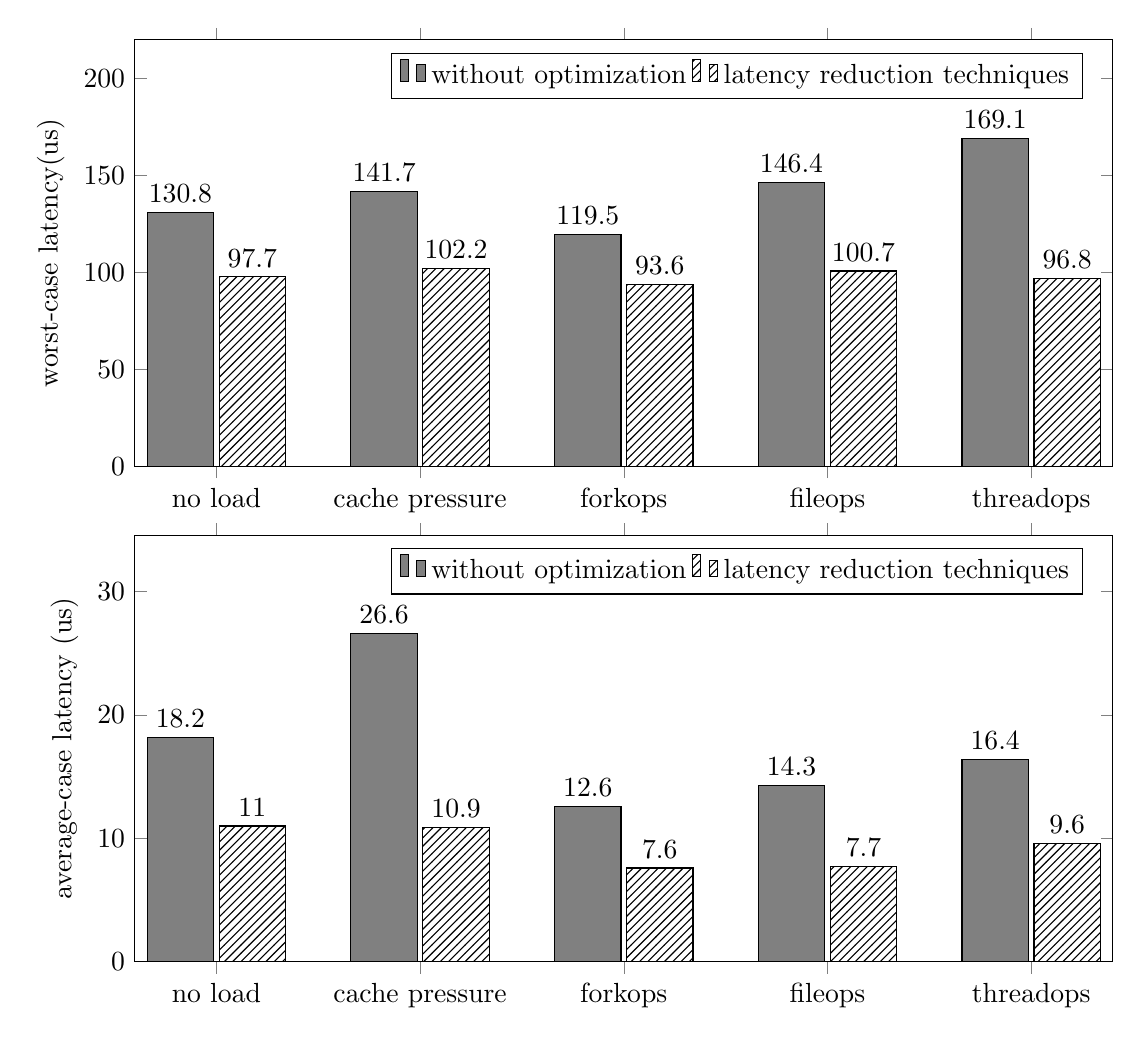
\begin{tikzpicture} %[scale = 1.2]

\begin{axis} [name=plot1, height=7cm, width=14cm, ybar=2pt, enlarge y limits={upper,value=0.3},  %enlargelimits=0.3, 
			ymin=0,
			legend pos=north east, legend columns=-1,
                       %legend style={at={(0.5,-0.1)}, anchor=north, legend columns=-1}, 
                       ylabel={worst-case latency(us)}, %title=no pollution from gp-guest, 
		       bar width= 24pt,
			%symbolic x coords={without VPID, with VPID},
                       symbolic x coords={no load, cache pressure, forkops, fileops, threadops},
                       xtick=data, nodes near coords, nodes near coords align={vertical}, x tick label style={rotate=0,anchor=north}, ]                    
	\addplot [fill=black!50] coordinates {
                    (no load,130.8) 
					(cache pressure,141.7)	
					(forkops,119.5)
					(fileops,146.4)
					(threadops,169.1)
			      };

	\addplot [postaction={pattern=north east lines}] coordinates {
                    (no load,97.7) 
					(cache pressure,102.2)	
					(forkops,93.6)
					(fileops,100.7)
					(threadops,96.8)
			      };
\legend{without optimization, latency reduction techniques}
\end{axis}


\begin{axis} [name=plot2, at={($(plot1.west)+(0,-9cm)$)}, height=7cm,  width=14cm, ybar=2pt, enlarge y limits={upper,value=0.3},  %enlargelimits=0.3, 
			ymin=0,
                       legend pos=north east, legend columns=-1,
			%legend style={at={(0.5,-0.1)}, anchor=north, legend columns=-1}, 
                       ylabel={average-case latency (us)}, %title=no pollution from gp-guest, 
		       bar width= 24pt,
                       %symbolic x coords={without VPID, with VPID},
			symbolic x coords={no load, cache pressure, forkops, fileops, threadops},
                       xtick=data, nodes near coords, nodes near coords align={vertical}, x tick label style={rotate=0,anchor=north}, ]                    
	\addplot [fill=black!50] coordinates {
                    (no load,18.2) 
					(cache pressure,26.6)	
					(forkops,12.6)
					(fileops,14.3)
					(threadops,16.4)			
			      };
	\addplot [postaction={pattern=north east lines}] 				
				coordinates {
                    (no load,11) 
					(cache pressure,10.9)	
					(forkops,7.6)
					(fileops,7.7)
					(threadops,9.6)			
			      };
\legend{without optimization, latency reduction techniques}
\end{axis}

\end{tikzpicture}

%\begin{tabular}{c c c c c}
%\multicolumn{5}{c}{Percentage Improvement}
%no load & cache pressure & forkops & fileops & threadops \\
%25.3 & 27.9 & 21.7 & 31.2 & 42.8 \\
%\end{tabular}

\end{center}
\ifreport
\caption{Comparison of interrupt latency when no optimization is deployed versus latency reduction techniques (direct interrupt, cache allocation, isolated TLB cache)}
\fi
\label{plot-allopt}
\end{figure}



The interrupt response time has improved approximately $30\%$ when latency reduction techniques are deployed.
The overall improvement with all optimization enabled look very similar to results for direct interrupt mechanism, however there is slight improvement in average-case and worst-case.

Figure \ref{plot-cdf-native-virtual-optimiz} plots CDF of gpio interrupt latency for three different setups: native, virtual with no optimization and virtual with latency reduction techniques. The interrupt latency is plotted for three different loads, same as in Figure \ref{plot-cdf-native-vs-virtual}.
The comparison of CDFs reveals improved average-case response time and reduced spread compared with virtualization overhead recorded in previous chapter.

\begin{figure}[!htb]
\begin{center}

\begin{tikzpicture}


\begin{axis}[name=plot1, height=6cm, width=12cm, ymin=0, ymax=1, xmin=0, 		
		xlabel=latency(us), 
		ylabel=probability,
		title style={yshift=-2ex},
		legend pos=south east,
		title=load:cache pressure,
		]
	\addplot [thick, blue] table[x=Latency,y=Probability] {./figures/native_cachepressure_10k_cdf.dat};
	\addplot [thick, red] table[x=Latency,y=Probability] {./figures/virt_cachepressure_10k_cdf.dat};
	\addplot [very thick, green] table[x=Latency,y=Probability] {./figures/allopt_cachepressure_10k_cdf.dat};
	\legend {\small{native (avg 44.2, max 77.9)}, \small{virtual (avg 18.2, max 131.1)}, \small{optimized (avg 11, max 100.4)}}
\end{axis}


\begin{axis}[name=plot2, at={($(plot1.south west)+(0,-6.5cm)$)}, height=6cm, width=12cm, ymin=0, ymax=1, xmin=0, 
		legend pos=south east,
		xlabel=latency(us), 
		ylabel=probability, 
		title style={yshift=-2ex},
		title=load:threadops,
		]
	\addplot [thick, blue] table[x=Latency,y=Probability] {./figures/native_threadops_cdf.dat};	
	\addplot [thick, red] table[x=Latency,y=Probability] {./figures/virt_threadops_10k_cdf.dat};
	\addplot [very thick, green] table[x=Latency,y=Probability] {./figures/allopt_threadops_10k_cdf.dat};
	\legend {\small{native (avg 5, max 12.4)}, \small{virtual (avg 16.4, max 169.1)}, \small{optimized (avg 9.6, max 96.8)}}
\end{axis}



\begin{axis}[name=plot3, at={($(plot2.south west)+(0,-6.5cm)$)}, height=6cm, width=12cm, ymin=0, ymax=1, xmin=0, 
		legend pos=south east,
		xlabel=latency(us), 
		ylabel=probability, 
		title style={yshift=-2ex},
		title=load:forkops,
		]
	\addplot [thick, blue] table[x=Latency,y=Probability] {./figures/native_forkops_10k_cdf.dat};	
	\addplot [thick, red] table[x=Latency,y=Probability] {./figures/virt_forkops2_10k_cdf.dat};
	\addplot [very thick, green] table[x=Latency,y=Probability] {./figures/allopt_forkops_10k_cdf.dat};
	\legend {\small{native (avg 6.1, max 25.9)}, \small{virtual (avg 12.6, max 119.5)}, \small{optimized (avg 7.6, max 97.7)}}
\end{axis}

\end{tikzpicture}
\end{center}
\ifreport
\caption{Comparison of interrupt latency CDF between native and virtual setup for different load conditions}
\fi
\label{plot-cdf-native-virtual-optimiz}
\end{figure}






\chapter{Related Work\label{chap5}}


This chapter will cover a brief introduction to related research work that has focused on virtualization solutions
for real-time applications by developing new or bringing real-time capabilities to existing virtualization
solutions. Furthermore, it presents some of the research efforts made to improve the responsiveness of real-time guests.

\section{KVM-based solutions}
Kernel-based Virtual Machine (KVM) is an open source type-2 hypervisor extensively used as virtualization solution in the enterprise domain \cite{kivity2007kvm}.
KVM uses existing Linux kernel mechanisms like scheduling policies etc. for virtual machines. 
Kiszka \cite{kiszka2009towards} has proposed real-time improvements that include using PREEMPT\_RT patch \cite{PREEMPT-RT} 
to add real-time capabilities to host Linux kernel.
Zhang et al. presented a real-time virtualization solution using KVM hypervisor on x86 platform \cite{zuo2010performance}.
Their solution consisted of an RTOS and a GPOS running in separate virtual machines. 
They applied two performance improvement mechanisms on host Linux kernel: CPU shielding and interrupt prioritization.
The performance tunings significantly improved worst-case interrupt response time of the RTOS guest.
Furthermore, they showed worst-case Process Dispatch Latency Time (PDLT) of PREEMPT\_RT patched Linux guest improved after using the performance tunings.

\section{Xen-based solutions}
Xen is a widely used open source type-1 hypervisor \cite{Barham:2003:XAV:1165389.945462}. 
Many research projects have been conducted so far to make Xen appropriate for real-time virtualization.
The split driver model for IO devices makes it challenging to use for real-time workloads \cite{Yoo:2011:TUI:2103799.2103816}.
Masrur et al. \cite{masrur2010vm} evaluated real-time performance of Xen SEDF scheduler and proposed PSEDF scheduler to separate
real-time domains from others. The showed that separating real-time domain from others can lower interrupt latencies and jitters.
Xi et al. have developed the RT-Xen framework to support real-time scheduling policies in Xen \cite{Xi:2011:RTR:2038642.2038651}.
The RT-Xen project extends Xen by appending new scheduling widely used in the real-time domain.

\section{Microkernel-Based Solutions}
Schild et al. \cite{schild2009faithful} used x86 virtualization extensions to run unmodified guest OS on L4/Fiasco microkernel.
They observed increased interrupt response times for real-time guest interrupts and showed that in certain cases the interrupt latency
can increase significantly.
Bruns et al. investigated the real-time performance of L4/Fiasco microkernel \cite{bruns2010evaluation}.
The measured interrupt latencies and context-switch times of real-time guest and used FreeRTOS \cite{freertos} as a reference.
The experiments showed that average execution times and interrupt latencies for real-time guest are significantly larger than the real-time kernel.
They observed cache contention as the main contributor to the virtualization overhead.


\section{Other solutions}
XtratuM is type-1 non-preemptive hypervisor that is designed specifically for real-time safety critical applications \cite{Carrascosa:2014:XHR:2668138.2668142}.
XtratuM deploys para-virtualization to achieve minimality. It provides a minimalistic set of hypercalls to guests for hardware interfacing.
It achieves deterministic performance by using static partitioning of resources allocated to each virtual machine.
The approach is very close to the one used by Phidias hypervisor.

Quest-V is an open source separation kernel that uses hardware assisted-virtualization to isolate guest in time and space \cite{West:2016:VSK:2966277.2935748}.
It supports applications of mixed-criticality by sandboxing a real-time guest partition on a multicore processor.
Quest-V uses static partitioning of hardware resources across guests to avoid traditional virtualization overheads.
It allows real-time guest OS to receive IO interrupts without hypervisor intervention and tries to avoid vmexits as much as possible.

Gordon et al. proposed exit-less interrupt (ELI) delivery mechanism to remove vmexits in situations where hypervisor intervention is not required \cite{Gordon:2012:EBP:2150976.2151020}.
Their solution is software-only where a shadow-IDT is maintained by the host to inject virtual interrupts to the unmodified guest.
They have shown ELI approach improves the throughput of IO-intensive workloads.


\chapter{Conclusion\label{chap6}}

This thesis analyzed real-time capabilities of Phidias hypervisor and performance improvement techniques.
The results showed that virtualization has increased real-time interrupt response times.
However, the overhead is bounded and can be reduced by applying performance improvement techniques.
Furthermore, there is still room for improvement and could be considered in future work.

Worst-case interrupt latency that was under $80us$ in native environment has increased more than twice in virtual environment and stayed under $170us$.
Investigation of overhead components revealed resource contention as main reason of increased interrupt latency.
The context-switch time for transitions to and from hypervisor can go as high as $86us$, which is purely hardware overhead.
CPU performance during the time when hypervisor runs can drop as low as one instruction completes in $77cc$ on average.
The study has presented enough evidence to conclude most part of the virtualization overhead is purely hardware overhead.

Interrupt response time of real-time guest interrupts improved significantly when latency reduction techniques were applied.
Direct interrupt injection lowered the interrupt latency by more than $25us$.
Isolating LLC of real-time guest from GPOS guest decreased interrupt latency by more than $15us$.
And TLB virtualization allowed latency reduction of more than $3.4us$.
When latency reduction techniques are used altogether, the virtualized solution can meet real-time constraints in the order of magnitude ($90us-110us$) which not far
from the native ($20us-80us$). 
Furthermore, during the study I found potential areas of improvement that could lead to further reduction of interrupt response times.


\section{Future Work}
This study focused on latency reduction techniques to improve real-time interrupt response time.
The analysis of overhead and latency reduction techniques revealed some areas that need to be investigated more.

Cache allocation used to lower interrupt latency was applied to shared L3 cache to separate traffic of RTOS and GPOS guest.
Since Phidias also executes on same core as real-time guest does, their data can interfere at L1
and L2 caches. Like L3 partitioning is supported in hardware, some x86 processors also support L2 partitioning.
Future work can use one of those processor to avoid interference between guest and hypervisor.
The x86 processor had multi-level big caches, these caches suffer from long miss penalties.
The work from this study can be repeated on processor with smaller caches to 
evaluate Phidias performance and see if long miss penalties are the major component of virtualization overhead.

While executing various kinds of loads on real-time guest, I observed frequent guest traps causing 
vm transitions. Frequent context-switching can result in pollution of caches already warmed-up for guest code.
Most transition are necessary, however current version of Phidias hypervisor uses VM configuration to
exit for all IO access, and accesses to all MSR.
The x86 VT-x enables host to use bitmasks to take exits only for an access that needs host attention.
Although I extended Phidias to use these mechanisms, but limited support could be added due to limitation of time.
More investigation is required to fully utilize these mechanisms and evaluate impact on virtualization overhead.



%%%%%%%%%%%%%%%%%%%%%%APPENDICES%%%%%%%%%%%%%%%%%%%%%
\appendix
\chapter{Code Fragments} \label{app:a}

\section{Kernel Patch for Fixed Clock Frequency and HPET Passthrough}
\begin{itemize}
	\item {\url{https://gitlab.sec.t-labs.tu-berlin.de/m.arshad/misc/blob/master/patches/clkfreqfix.patch}}
\end{itemize}	

\section{Kernel Patch for PCIe GPIO Device Passthrough}
\begin{itemize}
	\item {\url{https://gitlab.sec.t-labs.tu-berlin.de/m.arshad/misc/tree/master/patches/gpio}}
\end{itemize}	

\section{Kernel Module for GPIO Interrupt}
\begin{itemize}
	\item {\url{https://gitlab.sec.t-labs.tu-berlin.de/m.arshad/misc/tree/master/gpio/gpio_interrupt}}
\end{itemize}	

\section{Microbenchmarks}
\begin{itemize}	
	\item {\mthreadops{} and \mhackbench{}: \url{https://github.com/koppi/linux-rt-tests}}
	\item {\mcachepressure{}: \url{https://gitlab.sec.t-labs.tu-berlin.de/m.arshad/misc/tree/master/cache_pollution/l2cachepollute}}
	\item {other benchmarks: \url{https://gitlab.sec.t-labs.tu-berlin.de/m.arshad/misc/tree/master/synthetic-workloads}}
	\item {LLC pollution: \url{https://gitlab.sec.t-labs.tu-berlin.de/m.arshad/misc/tree/master/cache_pollution/l3cachepollute}}
\end{itemize}	


\section{External Measurement Setup}
\begin{itemize}
	\item{FPGA code:\url{https://gitlab.sec.t-labs.tu-berlin.de/m.arshad/misc/tree/master/fpga/latency}} 
	\item{Script:\url{https://gitlab.sec.t-labs.tu-berlin.de/m.arshad/misc/blob/master/fpga/latency/uart.py}} 
\end{itemize}	



\chapter{Phidias Runtime}  \label{app:b}

%\begin{table}[h]
%\centering
%\begin{longtable}{|p{.20\textwidth} | p{.70\textwidth}|}
%\begin{longtable}{|c|c|c|c|c|c|c|c|c|c|}  
%\hline
%\small{exit reason} & \small{external} & \small{cupid} & \small{crX} 
%& \small{io} & \small{rdmsr} & \small{wrmsr} & \small{eoi} & \small{ept} & \small{apic} \\
%\small{benchmark} & \small{interrupt} & \small{} & \small{access} 
%& \small{access} & \small{} & \small{} & \small{exit} & \small{violation} & \small{write} \\ \hline 
%\hline
%after bootup & 7075 & 323 & 11254 & 122577 & 4 & 7292 & 3 & 584 & 13 \\ \hline
%cache pressure & 5229 & 11572 & 4766 & 135 & 0 & 28555 & 9997 & 0 & 0 \\ \hline
%forkops & 143650 & 20 & 545662 & 35 & 0 & 681097 & 9994 & 0 & 0 \\ \hline
%fileops & 274394 & 19 & 6 & 35 & 0 & 681097 & 9994 & 0 & 0 \\ \hline
%hackbench & 40926 & 0 & 2018287 & 0 & 0 & 2064207 & 9990 & 0 & 0   \\ \hline
%mmapops & 47258 & 0 & 19758 & 0 & 0 & 123174 & 9990 & 0 & 0 \\ \hline
%stdout & 195436 & 19 & 6 & 154 & 0 & 770222 & 9990 & 0 & 0 \\ \hline
%threadops  & 158602 & 19 & 6 & 459 & 0 & 407221 & 9989 & 0 & 0 \\ \hline
%\caption{Phidias intervension during test} 
%\label{Phidias exit frequency}
%\end{longtable}
%\end{table}

\begin{longtable}{|r|c|c|c|c|c|}
%	\centering
	%\hline
	%\textbf{exit}	& \textbf{exit}	 & \textbf{min.} 	& \textbf{max.} & \textbf{avg.} & \textbf{instr.}  \\
	%\textbf{reason}	& \textbf{freq.} & \textbf{time} (cc)	& \textbf{time} (cc)	& \textbf{time} (cc)	& \textbf{retired}  \\ \hline

	 \hline
	\textbf{exit}	& \textbf{exit}	 & \textbf{min.} 	& \textbf{max.} & \textbf{avg.} & \textbf{instr.}  \\
	\textbf{reason}	& \textbf{freq.} & \textbf{time} (cc)	& \textbf{time} (cc)	& \textbf{time} (cc)	& \textbf{retired}  \\ \hline
	 \hline
	\endfirsthead

	 \hline
	\textbf{exit}	& \textbf{exit}	 & \textbf{min.} 	& \textbf{max.} & \textbf{avg.} & \textbf{instr.}  \\
	\textbf{reason}	& \textbf{freq.} & \textbf{time} (cc)	& \textbf{time} (cc)	& \textbf{time} (cc)	& \textbf{retired}  \\ \hline
	 \hline
	\endhead

	\multicolumn{6}{|c|}{\textbf{\mcachepressure{}}} \\ \hline
       ext\_interrupt	& 3429	& 680	& 7021	& 1725	& 779  \\
               cpuid	& 7638	& 573	& 1008	& 697	& 517  \\
          crx\_access	& 3158	& 358	& 30332	& 1014	& 551  \\
           io\_access	& 135	& 401	& 178716 & 16548 & 2322  \\
               wrmsr	& 25142	& 287	& 30575	& 834	& 779   \\ 
            eoi\_exit	& 9986	& 276	& 169281 & 477	& 20504  \\ \hline
	\multicolumn{6}{|c|}{\textbf{\mforkops{}}} \\ \hline
       ext\_interrupt	& 174258	& 641	& 189773	& 1702	& 12925 \\
               cpuid	& 19	& 680	& 1020	& 750	& 526 \\
          crx\_access	& 657946	& 306	& 158508	& 840	& 11572 \\
           io\_access	& 240	& 396	& 175702	& 9263	& 2301 \\
               wrmsr	& 827333	& 258	& 165704	& 508	& 18593 \\
            eoi\_exit	& 9993	& 314	& 27986	& 483	& 550 \\ \hline
	\multicolumn{6}{|c|}{\textbf{\mfileops{}}} \\ \hline
	  ext\_interrupt	& 273731	& 595	& 173298	& 1288	& 18922 \\
               cpuid	& 20	& 680	& 1025	& 750	& 526 \\
          crx\_access	& 6	& 629	& 1282	& 1071	& 551 \\
           io\_access	& 35	& 401	& 172375	& 8326	& 2280 \\
               wrmsr	& 718708	& 282	& 196490	& 698	& 12640 \\
            eoi\_exit	& 9985	& 267	& 30031	& 620	& 550 \\ \hline
	\multicolumn{6}{|c|}{\textbf{\mhackbench{}}} \\ \hline
       ext\_interrupt	& 45230	& 651	& 6460	& 1138	& 1069 \\
               cpuid	& 19	& 680	& 1003	& 741	& 526 \\ 
          crx\_access	& 2272384	& 268	& 150476	& 703	& 22033 \\ 
           io\_access	& 611	& 380	& 176205	& 23042	& 2301 \\
               wrmsr	& 2321823	& 216	& 149052	& 234	& 20198 \\
            eoi\_exit	& 9993	& 216	& 864	& 287	& 559 \\ \hline
	\multicolumn{6}{|c|}{\textbf{\mmmapops{}}} \\ \hline
       ext\_interrupt	& 50559	& 714	& 149292	& 1077	& 19426 \\
               cpuid	& 19	& 680	& 930	& 736	& 524 \\ 
          crx\_access	& 21054	& 276	& 148436	& 546	& 20032 \\
           io\_access	& 35	& 396	& 183566	& 7604	& 2364 \\ 
               wrmsr	& 131238	& 216	& 148856	& 469	& 20278 \\
            eoi\_exit	& 9984	& 208	& 724	& 296	& 559 \\ \hline
	\multicolumn{6}{|c|}{\textbf{\mstdout{}}} \\ \hline
       ext\_interrupt	& 192641	& 430	& 186435	& 1240	& 21429 \\
               cpuid	& 19	& 675	& 1030	& 759	& 526 \\
          crx\_access	& 6	& 556	& 1287	& 1056	& 551 \\
           io\_access	& 35	& 396	& 176710	& 8470	& 2322 \\
               wrmsr	& 756404	& 262	& 186014	& 708	& 19836 \\
            eoi\_exit	& 9993	& 267	& 27206	& 345	& 550 \\ \hline
	\multicolumn{6}{|c|}{\textbf{\mthreadops{}}} \\ \hline
       ext\_interrupt	& 189248	& 590	& 200313	& 1265	& 19804 \\ 
               cpuid	& 19	& 680	& 1207	& 771	& 517 \\ 
          crx\_access	& 6	& 595	& 1246	& 1051	& 551 \\ 
           io\_access	& 204	& 401	& 185776	& 19111	& 2385 \\
               wrmsr	& 506235	& 282	& 172878	& 624	& 18745 \\ 
            eoi\_exit	& 9985	& 272	& 29733	& 590	& 550 \\ \hline

\caption{Phidias runtime profiling information} 
\label{phidias-runtime-detailed}
\end{longtable}


\chapter{Additional Graphics}  \label{app:c}

\section{Latency CDF for Native versus Virtual Setup}
\begin{figure}[!htb]
\begin{center}

\begin{tikzpicture}

\begin{axis}[name=plot1, height=\figheightVOCDFApp, width=\figwidthVOCDFApp, ymin=0, ymax=1, xmin=0, 		
		xlabel=latency ($\mu{}s$), 
		ylabel=probability,
		title style={yshift=-2ex},
		legend pos=south east,
		title=no load,
		]
	\addplot [very thick, blue, dashed] table[x=Latency,y=Probability] {./figures/native_noload_10k_cdf.dat};
	\addplot [thick, red] table[x=Latency,y=Probability] {./figures/virt_noload_10k_cdf.dat};
	\legend {\small{native (avg 44.2, max 67.6)}, \small{virtual (avg 18.2, max 130.8)}}
\end{axis}


\begin{axis}[name=plot2, \atCmdVOCDFLowerPlotAApp , height=\figheightVOCDFApp, width=\figwidthVOCDFApp, ymin=0, ymax=1, xmin=0, 
		legend pos=south east,
		xlabel=latency ($\mu{}s$), 
		ylabel=probability, 
		title style={yshift=-2ex},
		title=load:fileops,
		]
	\addplot [very thick, blue, dashed] table[x=Latency,y=Probability] {./figures/native_fileops_cdf.dat};	
	\addplot [thick, red] table[x=Latency,y=Probability] {./figures/virt_fileops_10k_cdf.dat};
	\legend {\small{native (avg 6.1, max 24.7)}, \small{virtual (avg 14.3, max 146.4)}}
\end{axis}

\end{tikzpicture}
\end{center}
%\caption{Interrupt latency CDF  comparison for native and virutal setup}
\label{plot-cdf-native-vs-virtual-appendix1}
\end{figure}
	
\begin{figure}[!htb]
\begin{center}
\begin{tikzpicture}

	\begin{axis}[name=plot1, height=\figheightVOCDFApp, width=\figwidthVOCDFApp, ymin=0, ymax=1, xmin=0, 
		legend pos=south east,
		xlabel=latency ($\mu{}s$), 
		ylabel=probability, 
		title style={yshift=-2ex},
		title=load:hackbench,
		]
	\addplot [very thick, blue, dashed] table[x=Latency,y=Probability] {./figures/native_hackbench_10k_cdf.dat};	
	\addplot [thick, red] table[x=Latency,y=Probability] {./figures/virt_hackbench_10k_cdf.dat};
	\legend {\small{native (avg 4.5, max 9.3)}, \small{virtual (max 10,  106.7)}}
	\end{axis}

	\begin{axis}[name=plot2, \atCmdVOCDFLowerPlotAApp , height=\figheightVOCDFApp, width=\figwidthVOCDFApp, ymin=0, ymax=1, xmin=0, 
		legend pos=south east,
		xlabel=latency ($\mu{}s$), 
		ylabel=probability, 
		title style={yshift=-2ex},
		title=load:mmapops,
		]
	\addplot [very thick, blue, dashed] table[x=Latency,y=Probability] {./figures/native_mmapops_cdf.dat};	
	\addplot [thick, red] table[x=Latency,y=Probability] {./figures/virt_mmapops_10k_cdf.dat};
	\legend {\small{native (avg 4.4, max 23.4)}, \small{virtual (avg 8.1, max 106.6}}
	\end{axis}

   	\begin{axis}[name=plot3, \atCmdVOCDFLowerPlotBApp , height=\figheightVOCDFApp, width=\figwidthVOCDFApp, ymin=0, ymax=1, xmin=0, 
		legend pos=south east,
		xlabel=latency ($\mu{}s$), 
		ylabel=probability, 
		title style={yshift=-2ex},
		title=load:stdout,
		]
	\addplot [very thick, blue, dashed] table[x=Latency,y=Probability] {./figures/native_stdout_cdf.dat};	
	\addplot [thick, red] table[x=Latency,y=Probability] {./figures/virt_stdout_10k_cdf.dat};
	\legend {\small{native (avg 6.1, max 25.8)}, \small{virtual (avg 14.9, max 142.7)}}
	\end{axis}

\end{tikzpicture}
\end{center}

\caption{Interrupt latency CDF  comparison for native and virtual setup}
\label{plot-cdf-native-vs-virtual-appendix2}
\end{figure}

\clearpage
\section{Latency CDF for Optimized Virtual Setup}
\begin{figure}[!htb]
\begin{center}

\begin{tikzpicture}

	\begin{axis}[name=plot1, height=\figheightVOCDFApp, width=\figwidthVOCDFApp, ymin=0, ymax=1, xmin=0, 		
		xlabel=latency ($\mu{}s$), 
		ylabel=probability,
		title style={yshift=-2ex},
		legend pos=south east,
		title=no load,
		]
	\addplot [dashed, very thick, blue] table[x=Latency,y=Probability] {./figures/native_noload_10k_cdf.dat};
	\addplot [dotted, very thick, red] table[x=Latency,y=Probability] {./figures/virt_noload_10k_cdf.dat};
	\addplot [very thick, OliveGreen] table[x=Latency,y=Probability] {./figures/allopt_noload_10k_cdf.dat};
	\legend {\small{native (avg 44.2, max 67.6)}, \small{virtual (avg 18.2, max 130.8)}, \small{optimized (avg 11, max 97.7)}}
	\end{axis}

	\begin{axis}[name=plot2, \atCmdVOCDFLowerPlotAApp, height=\figheightVOCDFApp, width=\figwidthVOCDFApp, ymin=0, ymax=1, xmin=0, 
		legend pos=south east,
		xlabel=latency ($\mu{}s$), 
		ylabel=probability, 
		title style={yshift=-2ex},
		title=load:fileops,
		]
	\addplot [dashed, very thick, blue] table[x=Latency,y=Probability] {./figures/native_fileops_cdf.dat};	
	\addplot [dotted, very thick, red] table[x=Latency,y=Probability] {./figures/virt_fileops_10k_cdf.dat};
	\addplot [very thick, OliveGreen] table[x=Latency,y=Probability] {./figures/allopt_fileops_10k_cdf.dat};
	\legend {\small{native (avg 6.1, max 24.7)}, \small{virtual (avg 14.3, max 146.7)}, \small{optimized (avg 7.7, max 100.7)}}
	\end{axis}

\end{tikzpicture}
\end{center}
\caption{Interrupt latency CDF comparison for native, virtual and optimized setups}
\label{plot-cdf-native-virtual-optimiz-appendix}
\end{figure}



%\printnoidxglossary[type=\acronymtype,title=Abbreviations]
%\clearpage
%\chapter*{} \label{abreviations}
%\printacronyms[include-classes=abbrev,name=Abbreviations]
\chapter{Glossary} \label{glossary:c}
%\printglossaries[style=super, type=\acronymtype]
\printnoidxglossaries

% ---------------------------------------------------------------
%\backmatter
%\newgeometry{tmargin=2.8cm,bmargin=3.5cm,lmargin=4cm,rmargin=3cm}

%\bibliographystyle{ieeetr}

\glsaddall
\printbibliography[heading=bibintoc]
\end{document}
